\documentclass[11pt,a4paper]{article}

\usepackage{gastex}
\usepackage{etoolbox}
% \newcommand{\showLoesung}{2} %<---als Schalter
% \newcommand{\showInhalt}{1} %<---als Schalter

\usepackage{alltt,moreverb,amsmath,enumerate}
\usepackage[normalem]{ulem}
\usepackage[T1]{fontenc}
\usepackage{ae,aecompl} %helvet,mathptm
%\usepackage[left=15mm,right=15mm,top=20mm,bottom=20mm]{geometry}
\usepackage[margin=.5in]{geometry}
%\usepackage[latin1]{inputenc} % f�r Linux
\usepackage[utf8]{inputenc} % Umlaute etc. direkt schreiben (unter Windows)
\usepackage[german]{babel}
\usepackage[url]{oth-logoPNG}
%\usepackage{i2sym,i2ams}

\usepackage{tikz}
\usetikzlibrary{arrows,shapes,trees,positioning,automata,decorations.pathreplacing,decorations.pathmorphing}
\usepackage{tkz-graph}
\usepackage{color}

\usepackage{longtable}
\usepackage{tabularx}

%\usepackage{epic}
%\usepackage{eepic}
\usepackage{comment,ifthen}
\usepackage{../include/todo}

\usepackage[T1]{fontenc}
\usepackage{textcomp}

\usepackage{listings}                   % Listings in Core-Erlang und Maude
\usepackage{lstmisc}

\usepackage{epic}                       % Bildbefehle (picture)
%\usepackage{eepic}                      % erweiterte Bildbefehle

\usepackage{bbm}                        % Mengensymbole (N,C,R,B)
\usepackage{latexsym}                   % zusaetzliche Mathesymbole
\usepackage{amsmath}                    % Mathepaket von der AMS
\usepackage{amstext}
\usepackage{amsfonts}
\usepackage{stmaryrd}                   % zusaetzliche Mathesymbole
\usepackage{mathtools}
\usepackage{amsthm}
\usepackage{cancel}

\usepackage{hyperref}
\usepackage{url}                        % Zum Setzen von URLs in typewriter-face

\pagestyle{empty}

\let\epsilon=\varepsilon
\let\phi=\varphi

\frenchspacing

\setlength{\parindent}{0pt}
\setlength{\textwidth}{18.6cm}
\setlength{\textheight}{26.5cm}
\setlength{\hfuzz}{1mm}

%%% Read dates of assignments from file
\usepackage{xparse}
\ExplSyntaxOn
\ior_new:N \g_hringriin_file_stream

\NewDocumentCommand{\ReadFile}{mm}
 {
  \hringriin_read_file:nn { #1 } { #2 }
  \cs_new:Npn #1 ##1
   {
    \str_if_eq:nnTF { ##1 } { * }
      { \seq_count:c { g_hringriin_file_ \cs_to_str:N #1 _seq } }
      { \seq_item:cn { g_hringriin_file_ \cs_to_str:N #1 _seq } { ##1 } }
   }
 }

\cs_new_protected:Nn \hringriin_read_file:nn
 {
  \ior_open:Nn \g_hringriin_file_stream { #2 }
  \seq_gclear_new:c { g_hringriin_file_ \cs_to_str:N #1 _seq }
  \ior_map_inline:Nn \g_hringriin_file_stream
   {
    \seq_gput_right:cx 
     { g_hringriin_file_ \cs_to_str:N #1 _seq }
     { \tl_trim_spaces:n { ##1 } }
   }
  \ior_close:N \g_hringriin_file_stream
 }

\ExplSyntaxOff

\ReadFile{\uebungsabgabe}{../skel/UEBUNGSABGABE.def}

%%% Read subject info from file
\newcommand{\dozent}[1]{\def\DOZENT{#1}}
\newcommand{\tutoren}[1]{\def\TUTOREN{#1}}
\newcommand{\vorlesung}[1]{\def\VORLESUNG{#1}}
\newcommand{\semester}[1]{\def\SEMESTER{#1}}

\InputIfFileExists{../skel/VORLESUNG.def}{\providecommand{\TUTOREN}{}}%
{\typeout{***********}
 \typeout{Warnung: Kein File vorhanden, das die Vorlesung spezifiziert!}
 \typeout{Spezifikation muss daher im Text des Blattes oder ueber die
          Tastatur erfolgen.}
 \typeout{***********}}

\def\Uebung#1#2#3{
  \othLehrstuhlLogo[\DOZENT]
  \begin{center}
	{~\\[-2em]\Large\bf \VORLESUNG}\\[0.5em]
    \LARGE --~Tutorium #1 (Übung #2)~--\\[4mm]
  \
  \normalsize
  \textbf{#3}
    \rule{\textwidth}{0.1pt}\\[1cm]
  \end{center}
}

\def\Hinweis#1{
	{~\\[-3em]\bf Hinweis: }
	\begin{minipage}[t]{16.5cm}
	#1
	\end{minipage}\\[1em]
    \rule{\textwidth}{0.1pt}
}

\def\Tipps#1{
	{~\\[-3em]\bf Tipps: }
	\begin{minipage}[t]{16.5cm}
	#1
	\end{minipage}\\[1em]
    \rule{\textwidth}{0.1pt}
}
  
\def\MyHeader{
  \othLehrstuhlLogo[Prof.~Dr.~rer.~nat.~Carsten~Kern]%[Carsten~Kern,~Stefan~Rieger]
}

\newcommand{\sem}[1]{[\![#1\,]\!]}

\def\aufgabe#1#2{\subsection*{Aufgabe #1 (#2)}\par}
\def\endaufgabe{}

\newenvironment{loesung}{\subsection*{L\"osungsvorschlag:}}{}
\newenvironment{hinweis}{}{}
\ifthenelse{\isundefined{\showLoesung}}{\excludecomment{loesung}}{\pagestyle{plain}\excludecomment{hinweis}}

\newenvironment{tipps}{}{}
\ifthenelse{\isundefined{\showTipps}}{\excludecomment{tipps}}{\excludecomment{hinweis}}

\newenvironment{inhalt}{\subsection*{Kommentar:}}{}
\ifthenelse{\isundefined{\showInhalt}}{\excludecomment{inhalt}}{}

\long\def\Exercise#1#2{\begin{exercise}{#1}#2\end{exercise}}

\def\underbar#1{%
  \setbox0=\hbox{#1}%
  \dimen0=\dp0\relax%
  \dp0=0pt%
  \setbox0=\hbox{\underline{\box0}}%
  \dp0=\dimen0\relax%
  \box0%
  }

\makeatletter
\def\@makeunderbar[#1]#2{\expandafter\def\csname#1\endcsname{\underbar{#2}}}
\def\makeunderbar{\@ifnextchar[{\@makeunderbar}{\@makeunderbar[]}}
\makeatother

\def\T{\mathrm{T}}
\def\P{\mathrm{P}}
\def\CT{\mathrm{CT}}
\def\COp{\mathrm{COp}}

\makeunderbar{Comp}
\makeunderbar{Ops}
\makeunderbar{trans}
\makeunderbar[strans]{s-trans}
\makeunderbar[ntrans]{n-trans}
\makeunderbar{fix}

\def\labelenumi{\alph{enumi})}
\let\<=\langle
\let\>=\rangle

\parindent=0pt
\parskip=1ex

\definecolor{javared}{rgb}{0.6,0,0} % for strings
\definecolor{javagreen}{rgb}{0.25,0.5,0.35} % comments
\definecolor{javapurple}{rgb}{0.5,0,0.35} % keywords
\definecolor{javadocblue}{rgb}{0.25,0.35,0.75} % javadoc
 
\lstset{language=C++,
basicstyle=\ttfamily\footnotesize,
keywordstyle=\color{javapurple}\bf,
stringstyle=\color{javared},
commentstyle=\color{javagreen}\it\bf,
morecomment=[s][\color{javadocblue}]{/**}{*/},
numbers=left,
numberstyle=\tiny\color{gray},
stepnumber=1,
numbersep=10pt,
tabsize=3,
showspaces=false,
showstringspaces=false}

\usepackage{enumitem}
\usepackage{algpseudocode}
\usepackage{caption}
\usepackage{subcaption}
\usepackage{placeins}
\usepackage{multicol}
\usepackage{slashbox}
\usepackage{fancyvrb}
\usepackage{ulem}
\usepackage{amssymb}

\begin{document}
\thispagestyle{empty}
\DeclareRobustCommand{\ttfamily}{\fontencoding{T1}\fontfamily{lmtt}\selectfont}

\newcommand{\quotes}[1]{\glqq{}#1\grqq{}}

\Uebung{11}{12}{Simon Thelen}{13. Januar 2021}  % FIXME: Blattnummer, Datum, Zeit

%%%%%%%%%%%%%%%%%%%%%%%%%%%%%%%%%%%%%%%%%%%%%%%%%%%%%%%%%%%%%%%%%%%%%%

\ifcsdef{showLoesung}{
\textbf{Bitte beachten Sie:} Die Lösungen können trotz sorgfältiger Prüfung Fehler enthalten.
Bei Fragen oder Unklarheiten kontaktieren Sie bitte den Tutor oder Dozenten in Tutorien, Übungen oder nach Vorlesungen.
}{}

\begin{aufgabe}{1}{Tiefensuche}
    \begin{enumerate}
        \item Zeigen oder widerlegen Sie folgende Aussage:
        \emph{Wenn während einer Tiefensuche auf einem ungerichteten Graphen eine Kante $\{u, v\}$ zum ersten Mal und zwar von $u$ aus betrachtet wird, ist $v$ niemals schwarz.}
        \item Zeigen oder widerlegen Sie folgende Aussage:
        \emph{Wenn während einer Tiefensuche auf einem gerichteten, azyklischen Graphen eine Kante $(u, v)$ von $u$ aus betrachtet wird, ist $v$ niemals grau.}
    \end{enumerate}
\end{aufgabe}

\begin{loesung}
    \begin{enumerate}
        % \item Die Aussage ist falsch.
        % \begin{proof}
        %     Beweis durch Gegenbeispiel:
        %     \begin{figure}[h!]
        %         \centering
        %         \begin{tikzpicture}[scale=0.12]
        %             \tikzstyle{every node}+=[inner sep=0pt]
        %             \draw [black] (26.7,-19.9) circle (3);
        %             \draw (26.7,-19.9) node {$1$};
        %             \draw [black] (37.9,-19.9) circle (3);
        %             \draw (37.9,-19.9) node {$2$};
        %             \draw [black] (48.8,-19.9) circle (3);
        %             \draw (48.8,-19.9) node {$3$};
        %             \draw [black] (29.7,-19.9) -- (34.9,-19.9);
        %             \draw [black] (40.9,-19.9) -- (45.8,-19.9);
        %             \draw [black] (28.753,-17.72) arc (130.51772:49.48228:13.849);
        %         \end{tikzpicture}
        %     \end{figure}
        %     \FloatBarrier
        %     Es wird eine Tiefensuche bei Knoten 1 gestartet und die Kante $\{1, 2\}$ zuerst traversiert und als nächstes Knoten 2 untersucht.
        %     Anschließend muss die Kante $\{2, 3\}$ traversiert werden, also wird nun Knoten 3 untersucht.
        %     Zu diesem Zeitpunkt sind alle Knoten grau.
        %     Daher wird Knoten 3 abgeschlossen.
        %     Anschließend wird Knoten 2 abgeschlossen.
        %     Bevor auch Knoten 1 abgeschlossen werden kann, muss noch Kante $\{1, 3\}$ überprüft werden.
        %     Zu diesem Zeitpunkt ist jedoch Knoten 3 bereits abgeschlossen und damit schwarz.
        % \end{proof}
        \item
        Die Aussage ist richtig.
        \begin{proof}
            Beweis durch Widerspruch:
            Angenommen wir traversieren $\{u, v\}$ zum ersten Mal und $v$ ist schwarz.
            Das bedeutet, $v$ ist abgeschlossen und alle von $v$ ausgehenden Kanten wurden bereits betrachtet.
            Da der Graph ungerichtet ist, gehört auch $\{u, v\}$ dazu.
            Das bedeutet $\{u, v\}$ wurde bereits betrachtet.
            Dies stellt einen Widerspruch zur Annahme dar, dass wir $\{u, v\}$ zum ersten Mal traversieren.
        \end{proof}
        \item Die Aussage ist richtig.
        \begin{proof}
            Beweis durch Widerspruch:
            Angenommen, eine Tiefensuche wird auf einem gerichteten, azyklischen Graphen ausgeführt und dabei wird eine Kante $(u, v)$ überprüft, wobei Knoten $v$ grau ist.
            Also wird gerade $u$ untersucht, während $v$ noch nicht abgeschlossen ist.
            $u$ liegt also im Tiefensuchenbaum im Teilbaum unter $v$.
            Das bedeutet, es gibt es einen direkten Pfad von $v$ nach $u$.
            Die Kante $(u, v)$ schließt somit einen Zyklus.
            Der Graph ist also nicht azyklisch, was einen Widerspruch zur Annahme darstellt.
        \end{proof}
    \end{enumerate}
\end{loesung}

\begin{aufgabe}{2}{Minimale Spannbäume}
    Gegeben seien folgende, ungerichtete Graphen:
    \begin{figure}[h!]
        \centering
        $G_1$:
        \begin{subfigure}{0.34\textwidth}
            \centering
            \begin{tikzpicture}[scale=0.15]
                \tikzstyle{every node}+=[inner sep=0pt]
                \draw [black] (20.9,-19.3) circle (3);
                \draw (20.9,-19.3) node {$1$};
                \draw [black] (34.9,-19.3) circle (3);
                \draw (34.9,-19.3) node {$2$};
                \draw [black] (21.1,-32.2) circle (3);
                \draw (21.1,-32.2) node {$4$};
                \draw [black] (48.6,-19.3) circle (3);
                \draw (48.6,-19.3) node {$3$};
                \draw [black] (48.6,-32.2) circle (3);
                \draw (48.6,-32.2) node {$6$};
                \draw [black] (34.9,-32.2) circle (3);
                \draw (34.9,-32.2) node {$5$};
                \draw [black] (23.9,-19.3) -- (31.9,-19.3);
                \draw (27.9,-18.8) node [above] {$1$};
                \draw [black] (20.95,-22.3) -- (21.05,-29.2);
                \draw (20.48,-25.75) node [left] {$1$};
                \draw [black] (48.6,-22.3) -- (48.6,-29.2);
                \draw (48.1,-25.75) node [left] {$2$};
                \draw [black] (32.71,-21.35) -- (23.29,-30.15);
                \draw (26.98,-25.27) node [above] {$2$};
                \draw [black] (37.08,-21.36) -- (46.42,-30.14);
                \draw (42.77,-25.27) node [above] {$3$};
                \draw [black] (24.1,-32.2) -- (31.9,-32.2);
                \draw (28,-31.7) node [above] {$3$};
                \draw [black] (34.9,-29.2) -- (34.9,-22.3);
                \draw (35.4,-25.75) node [right] {$4$};
                \draw [black] (37.9,-19.3) -- (45.6,-19.3);
                \draw (41.75,-18.8) node [above] {$4$};
                \draw [black] (37.9,-32.2) -- (45.6,-32.2);
                \draw (41.75,-31.7) node [above] {$4$};
            \end{tikzpicture}
        \end{subfigure}
        $G_2$:
        \begin{subfigure}{0.34\textwidth}
            \centering
            \begin{tikzpicture}[scale=0.13]
                \tikzstyle{every node}+=[inner sep=0pt]
                \draw [black] (16.1,-16.8) circle (3);
                \draw (16.1,-16.8) node {$1$};
                \draw [black] (32.1,-16.8) circle (3);
                \draw (32.1,-16.8) node {$2$};
                \draw [black] (16.1,-31.8) circle (3);
                \draw (16.1,-31.8) node {$4$};
                \draw [black] (32.1,-31.8) circle (3);
                \draw (32.1,-31.8) node {$5$};
                \draw [black] (47.8,-31.8) circle (3);
                \draw (47.8,-31.8) node {$6$};
                \draw [black] (47.8,-16.8) circle (3);
                \draw (47.8,-16.8) node {$3$};
                \draw [black] (16.1,-47.2) circle (3);
                \draw (16.1,-47.2) node {$7$};
                \draw [black] (32.1,-47.2) circle (3);
                \draw (32.1,-47.2) node {$8$};
                \draw [black] (47.8,-47.2) circle (3);
                \draw (47.8,-47.2) node {$9$};
                \draw [black] (34.27,-29.73) -- (45.63,-18.87);
                \draw (38.93,-23.82) node [above] {$1$};
                \draw [black] (44.8,-31.8) -- (35.1,-31.8);
                \draw (39.95,-31.3) node [above] {$2$};
                \draw [black] (47.8,-28.8) -- (47.8,-19.8);
                \draw (47.3,-24.3) node [left] {$3$};
                \draw [black] (19.1,-47.2) -- (29.1,-47.2);
                \draw (24.1,-46.7) node [above] {$4$};
                \draw [black] (18.29,-29.75) -- (29.91,-18.85);
                \draw (23.08,-23.82) node [above] {$5$};
                \draw [black] (19.1,-31.8) -- (29.1,-31.8);
                \draw (24.1,-31.3) node [above] {$6$};
                \draw [black] (16.1,-34.8) -- (16.1,-44.2);
                \draw (15.6,-39.5) node [left] {$7$};
                \draw [black] (32.1,-34.8) -- (32.1,-44.2);
                \draw (31.6,-39.5) node [left] {$8$};
                \draw [black] (35.1,-16.8) -- (44.8,-16.8);
                \draw (39.95,-16.3) node [above] {$9$};
                \draw [black] (19.1,-16.8) -- (29.1,-16.8);
                \draw (24.1,-16.3) node [above] {$10$};
                \draw [black] (16.1,-19.8) -- (16.1,-28.8);
                \draw (15.6,-24.3) node [left] {$11$};
                \draw [black] (47.8,-34.8) -- (47.8,-44.2);
                \draw (47.3,-39.5) node [left] {$13$};
                \draw [black] (35.1,-47.2) -- (44.8,-47.2);
                \draw (39.95,-46.7) node [above] {$14$};
                \draw [black] (34.24,-45.1) -- (45.66,-33.9);
                \draw (38.43,-39.02) node [above] {$12$};
                \draw [black] (18.26,-45.12) -- (29.94,-33.88);
                \draw (22.58,-39.02) node [above] {$15$};
                \draw [black] (32.1,-28.8) -- (32.1,-19.8);
                \draw (31.6,-24.3) node [left] {$16$};
            \end{tikzpicture}
        \end{subfigure}
    \end{figure}
    \FloatBarrier
    \begin{enumerate}[label=\alph*)]
        \item Demonstieren Sie den Algorithmus von Kruskal zum Finden von minimalen Spannbäumen an $G_1$ (und optional $G_2$) nach dem Schema aus der Vorlesung.
        Geben Sie für jeden Zwischenschritt den bisherigen Teil-MST sowie den aktuellen Zustand der Union-Find-Datenstruktur an.
        \item Demonstieren Sie den Algorithmus von Prim zum Finden von minimalen Spannbäumen an $G_1$ (und optional $G_2$) nach dem Schema aus der Vorlesung.
        Starten Sie jeweils bei Knoten 1.
        Geben Sie für jeden Zwischenschritt den bisherigen Teil-MST sowie den aktuellen Zustand des Min-Heaps an.
        \item Angenommen, für einen Graph $G=(V,E)$ gilt $\forall \{u, v\} \in E$: $w(u, v) \in \{1, 2, \ldots, |E|\}$.
        Wie kann man den Algorithmus von Kruskal in einem solchen Fall mithilfe eines anderen Sortieralgorithmus beschleunigen?
        Welche Laufzeit hat Kruskal dann?
        \item\label{connected_components}Ein ungerichteter (nicht unbedingt zusammenhängender) Graph lässt sich in disjunkte \emph{Zusammenhangskomponenten} aufteilen, wobei sich in der Komponente, in der der Knoten $v$ liegt, genau die von $v$ aus erreichbaren Knoten befinden.
        Implementieren Sie einen Algorithmus in Pseudocode oder einer Programmiersprache Ihrer Wahl auf Basis der Union-Find-Datenstruktur aus der Vorlesung, der alle Zusammenhangskomponenten eines ungerichteten Graphen findet.
        Welche Worst-Case-Laufzeit hat Ihr Algorithmus?
        \item
        Wie können Sie das Problem aus Teilaufgabe \ref*{connected_components} schneller, nämlich in $O(|V| + |E|)$, mit einem Ihnen aus der Vorlesung bekannten Graphalgorithmus lösen?
    \end{enumerate}
\end{aufgabe}

\begin{loesung}
    \begin{enumerate}
        \item $G_1$:
        \begin{figure}[h!]
            \centering
            \begin{subfigure}[b]{0.34\textwidth}
                \centering
                \begin{tikzpicture}[scale=0.15]
                    \tikzstyle{every node}+=[inner sep=0pt]
                    \draw [black] (20.9,-19.3) circle (3);
                    \draw (20.9,-19.3) node {$1$};
                    \draw [black] (34.9,-19.3) circle (3);
                    \draw (34.9,-19.3) node {$2$};
                    \draw [black] (21.1,-32.2) circle (3);
                    \draw (21.1,-32.2) node {$4$};
                    \draw [black] (48.6,-19.3) circle (3);
                    \draw (48.6,-19.3) node {$3$};
                    \draw [black] (48.6,-32.2) circle (3);
                    \draw (48.6,-32.2) node {$6$};
                    \draw [black] (34.9,-32.2) circle (3);
                    \draw (34.9,-32.2) node {$5$};
                    \draw [black] (23.9,-19.3) -- (31.9,-19.3);
                    \draw (27.9,-18.8) node [above] {$1$};
                    \draw [black] (20.95,-22.3) -- (21.05,-29.2);
                    \draw (20.48,-25.75) node [left] {$1$};
                    \draw [black] (48.6,-22.3) -- (48.6,-29.2);
                    \draw (48.1,-25.75) node [left] {$2$};
                    \draw [black] (32.71,-21.35) -- (23.29,-30.15);
                    \draw (26.98,-25.27) node [above] {$2$};
                    \draw [black] (37.08,-21.36) -- (46.42,-30.14);
                    \draw (42.77,-25.27) node [above] {$3$};
                    \draw [black] (24.1,-32.2) -- (31.9,-32.2);
                    \draw (28,-31.7) node [above] {$3$};
                    \draw [black] (34.9,-29.2) -- (34.9,-22.3);
                    \draw (35.4,-25.75) node [right] {$4$};
                    \draw [black] (37.9,-19.3) -- (45.6,-19.3);
                    \draw (41.75,-18.8) node [above] {$4$};
                    \draw [black] (37.9,-32.2) -- (45.6,-32.2);
                    \draw (41.75,-31.7) node [above] {$4$};
                \end{tikzpicture}
            \end{subfigure}
            \begin{subfigure}[b]{0.34\textwidth}
                \centering
                \begin{tikzpicture}[scale=0.15]
                    \tikzstyle{every node}+=[inner sep=0pt]
                    \draw [black] (21.1,-19.3) circle (3);
                    \draw (21.1,-19.3) node {$1$};
                    \draw [black] (34,-19.3) circle (3);
                    \draw (34,-19.3) node {$2$};
                    \draw [black] (21.1,-32.2) circle (3);
                    \draw (21.1,-32.2) node {$4$};
                    \draw [black] (48.6,-19.3) circle (3);
                    \draw (48.6,-19.3) node {$3$};
                    \draw [black] (48.6,-32.2) circle (3);
                    \draw (48.6,-32.2) node {$6$};
                    \draw [black] (34.9,-32.2) circle (3);
                    \draw (34.9,-32.2) node {$5$};
                    \draw [black] (19.777,-16.62) arc (234:-54:2.25);
                    \fill [black] (22.42,-16.62) -- (23.3,-16.27) -- (22.49,-15.68);
                    \draw [black] (32.677,-16.62) arc (234:-54:2.25);
                    \fill [black] (35.32,-16.62) -- (36.2,-16.27) -- (35.39,-15.68);
                    \draw [black] (47.277,-16.62) arc (234:-54:2.25);
                    \fill [black] (49.92,-16.62) -- (50.8,-16.27) -- (49.99,-15.68);
                    \draw [black] (19.777,-29.52) arc (234:-54:2.25);
                    \fill [black] (22.42,-29.52) -- (23.3,-29.17) -- (22.49,-28.58);
                    \draw [black] (33.577,-29.52) arc (234:-54:2.25);
                    \fill [black] (36.22,-29.52) -- (37.1,-29.17) -- (36.29,-28.58);
                    \draw [black] (47.277,-29.52) arc (234:-54:2.25);
                    \fill [black] (49.92,-29.52) -- (50.8,-29.17) -- (49.99,-28.58);
                    % \draw [black] (31,-19.3) -- (24.1,-19.3);
                    % \fill [black] (24.1,-19.3) -- (24.9,-19.8) -- (24.9,-18.8);
                    % \draw [black] (21.1,-29.2) -- (21.1,-22.3);
                    % \fill [black] (21.1,-22.3) -- (20.6,-23.1) -- (21.6,-23.1);
                    % \draw [black] (48.6,-29.2) -- (48.6,-22.3);
                    % \fill [black] (48.6,-22.3) -- (48.1,-23.1) -- (49.1,-23.1);
                    % \draw [black] (23.615,-17.669) arc (119.23165:60.76835:23.006);
                    % \fill [black] (23.62,-17.67) -- (24.56,-17.71) -- (24.07,-16.84);
                    % \draw [black] (32.71,-30.15) -- (23.29,-21.35);
                    % \fill [black] (23.29,-21.35) -- (23.53,-22.26) -- (24.22,-21.53);
                \end{tikzpicture}
            \end{subfigure}
        \end{figure}
        \begin{figure}[h!]
            \centering
            \begin{subfigure}[b]{0.34\textwidth}
                \centering
                \begin{tikzpicture}[scale=0.15]
                    \tikzstyle{every node}+=[inner sep=0pt]
                    \draw [black] (20.9,-19.3) circle (3);
                    \draw (20.9,-19.3) node {$1$};
                    \draw [black] (34.9,-19.3) circle (3);
                    \draw (34.9,-19.3) node {$2$};
                    \draw [black] (21.1,-32.2) circle (3);
                    \draw (21.1,-32.2) node {$4$};
                    \draw [black] (48.6,-19.3) circle (3);
                    \draw (48.6,-19.3) node {$3$};
                    \draw [black] (48.6,-32.2) circle (3);
                    \draw (48.6,-32.2) node {$6$};
                    \draw [black] (34.9,-32.2) circle (3);
                    \draw (34.9,-32.2) node {$5$};
                    \draw [black, dashed] (23.9,-19.3) -- (31.9,-19.3);
                    \draw (27.9,-18.8) node [above] {$1$};
                    \draw [black] (20.95,-22.3) -- (21.05,-29.2);
                    \draw (20.48,-25.75) node [left] {$1$};
                    \draw [black] (48.6,-22.3) -- (48.6,-29.2);
                    \draw (48.1,-25.75) node [left] {$2$};
                    \draw [black] (32.71,-21.35) -- (23.29,-30.15);
                    \draw (26.98,-25.27) node [above] {$2$};
                    \draw [black] (37.08,-21.36) -- (46.42,-30.14);
                    \draw (42.77,-25.27) node [above] {$3$};
                    \draw [black] (24.1,-32.2) -- (31.9,-32.2);
                    \draw (28,-31.7) node [above] {$3$};
                    \draw [black] (34.9,-29.2) -- (34.9,-22.3);
                    \draw (35.4,-25.75) node [right] {$4$};
                    \draw [black] (37.9,-19.3) -- (45.6,-19.3);
                    \draw (41.75,-18.8) node [above] {$4$};
                    \draw [black] (37.9,-32.2) -- (45.6,-32.2);
                    \draw (41.75,-31.7) node [above] {$4$};
                \end{tikzpicture}
            \end{subfigure}
            \begin{subfigure}[b]{0.34\textwidth}
                \centering
                \begin{tikzpicture}[scale=0.15]
                    \tikzstyle{every node}+=[inner sep=0pt]
                    \draw [black] (21.1,-19.3) circle (3);
                    \draw (21.1,-19.3) node {$1$};
                    \draw [black] (34,-19.3) circle (3);
                    \draw (34,-19.3) node {$2$};
                    \draw [black] (21.1,-32.2) circle (3);
                    \draw (21.1,-32.2) node {$4$};
                    \draw [black] (48.6,-19.3) circle (3);
                    \draw (48.6,-19.3) node {$3$};
                    \draw [black] (48.6,-32.2) circle (3);
                    \draw (48.6,-32.2) node {$6$};
                    \draw [black] (34.9,-32.2) circle (3);
                    \draw (34.9,-32.2) node {$5$};
                    \draw [black] (19.777,-16.62) arc (234:-54:2.25);
                    \fill [black] (22.42,-16.62) -- (23.3,-16.27) -- (22.49,-15.68);
                    % \draw [black] (32.677,-16.62) arc (234:-54:2.25);
                    % \fill [black] (35.32,-16.62) -- (36.2,-16.27) -- (35.39,-15.68);
                    \draw [black] (47.277,-16.62) arc (234:-54:2.25);
                    \fill [black] (49.92,-16.62) -- (50.8,-16.27) -- (49.99,-15.68);
                    \draw [black] (19.777,-29.52) arc (234:-54:2.25);
                    \fill [black] (22.42,-29.52) -- (23.3,-29.17) -- (22.49,-28.58);
                    \draw [black] (33.577,-29.52) arc (234:-54:2.25);
                    \fill [black] (36.22,-29.52) -- (37.1,-29.17) -- (36.29,-28.58);
                    \draw [black] (47.277,-29.52) arc (234:-54:2.25);
                    \fill [black] (49.92,-29.52) -- (50.8,-29.17) -- (49.99,-28.58);
                    \draw [black] (31,-19.3) -- (24.1,-19.3);
                    \fill [black] (24.1,-19.3) -- (24.9,-19.8) -- (24.9,-18.8);
                    % \draw [black] (21.1,-29.2) -- (21.1,-22.3);
                    % \fill [black] (21.1,-22.3) -- (20.6,-23.1) -- (21.6,-23.1);
                    % \draw [black] (48.6,-29.2) -- (48.6,-22.3);
                    % \fill [black] (48.6,-22.3) -- (48.1,-23.1) -- (49.1,-23.1);
                    % \draw [black] (23.615,-17.669) arc (119.23165:60.76835:23.006);
                    % \fill [black] (23.62,-17.67) -- (24.56,-17.71) -- (24.07,-16.84);
                    % \draw [black] (32.71,-30.15) -- (23.29,-21.35);
                    % \fill [black] (23.29,-21.35) -- (23.53,-22.26) -- (24.22,-21.53);
                \end{tikzpicture}
            \end{subfigure}
        \end{figure}
        \begin{figure}[h!]
            \centering
            \begin{subfigure}[b]{0.34\textwidth}
                \centering
                \begin{tikzpicture}[scale=0.15]
                    \tikzstyle{every node}+=[inner sep=0pt]
                    \draw [black] (20.9,-19.3) circle (3);
                    \draw (20.9,-19.3) node {$1$};
                    \draw [black] (34.9,-19.3) circle (3);
                    \draw (34.9,-19.3) node {$2$};
                    \draw [black] (21.1,-32.2) circle (3);
                    \draw (21.1,-32.2) node {$4$};
                    \draw [black] (48.6,-19.3) circle (3);
                    \draw (48.6,-19.3) node {$3$};
                    \draw [black] (48.6,-32.2) circle (3);
                    \draw (48.6,-32.2) node {$6$};
                    \draw [black] (34.9,-32.2) circle (3);
                    \draw (34.9,-32.2) node {$5$};
                    \draw [black, dashed] (23.9,-19.3) -- (31.9,-19.3);
                    \draw (27.9,-18.8) node [above] {$1$};
                    \draw [black, dashed] (20.95,-22.3) -- (21.05,-29.2);
                    \draw (20.48,-25.75) node [left] {$1$};
                    \draw [black] (48.6,-22.3) -- (48.6,-29.2);
                    \draw (48.1,-25.75) node [left] {$2$};
                    \draw [black] (32.71,-21.35) -- (23.29,-30.15);
                    \draw (26.98,-25.27) node [above] {$2$};
                    \draw [black] (37.08,-21.36) -- (46.42,-30.14);
                    \draw (42.77,-25.27) node [above] {$3$};
                    \draw [black] (24.1,-32.2) -- (31.9,-32.2);
                    \draw (28,-31.7) node [above] {$3$};
                    \draw [black] (34.9,-29.2) -- (34.9,-22.3);
                    \draw (35.4,-25.75) node [right] {$4$};
                    \draw [black] (37.9,-19.3) -- (45.6,-19.3);
                    \draw (41.75,-18.8) node [above] {$4$};
                    \draw [black] (37.9,-32.2) -- (45.6,-32.2);
                    \draw (41.75,-31.7) node [above] {$4$};
                \end{tikzpicture}
            \end{subfigure}
            \begin{subfigure}[b]{0.34\textwidth}
                \centering
                \begin{tikzpicture}[scale=0.15]
                    \tikzstyle{every node}+=[inner sep=0pt]
                    \draw [black] (21.1,-19.3) circle (3);
                    \draw (21.1,-19.3) node {$1$};
                    \draw [black] (34,-19.3) circle (3);
                    \draw (34,-19.3) node {$2$};
                    \draw [black] (21.1,-32.2) circle (3);
                    \draw (21.1,-32.2) node {$4$};
                    \draw [black] (48.6,-19.3) circle (3);
                    \draw (48.6,-19.3) node {$3$};
                    \draw [black] (48.6,-32.2) circle (3);
                    \draw (48.6,-32.2) node {$6$};
                    \draw [black] (34.9,-32.2) circle (3);
                    \draw (34.9,-32.2) node {$5$};
                    \draw [black] (19.777,-16.62) arc (234:-54:2.25);
                    \fill [black] (22.42,-16.62) -- (23.3,-16.27) -- (22.49,-15.68);
                    % \draw [black] (32.677,-16.62) arc (234:-54:2.25);
                    % \fill [black] (35.32,-16.62) -- (36.2,-16.27) -- (35.39,-15.68);
                    \draw [black] (47.277,-16.62) arc (234:-54:2.25);
                    \fill [black] (49.92,-16.62) -- (50.8,-16.27) -- (49.99,-15.68);
                    % \draw [black] (19.777,-29.52) arc (234:-54:2.25);
                    % \fill [black] (22.42,-29.52) -- (23.3,-29.17) -- (22.49,-28.58);
                    \draw [black] (33.577,-29.52) arc (234:-54:2.25);
                    \fill [black] (36.22,-29.52) -- (37.1,-29.17) -- (36.29,-28.58);
                    \draw [black] (47.277,-29.52) arc (234:-54:2.25);
                    \fill [black] (49.92,-29.52) -- (50.8,-29.17) -- (49.99,-28.58);
                    \draw [black] (31,-19.3) -- (24.1,-19.3);
                    \fill [black] (24.1,-19.3) -- (24.9,-19.8) -- (24.9,-18.8);
                    \draw [black] (21.1,-29.2) -- (21.1,-22.3);
                    \fill [black] (21.1,-22.3) -- (20.6,-23.1) -- (21.6,-23.1);
                    % \draw [black] (48.6,-29.2) -- (48.6,-22.3);
                    % \fill [black] (48.6,-22.3) -- (48.1,-23.1) -- (49.1,-23.1);
                    % \draw [black] (23.615,-17.669) arc (119.23165:60.76835:23.006);
                    % \fill [black] (23.62,-17.67) -- (24.56,-17.71) -- (24.07,-16.84);
                    % \draw [black] (32.71,-30.15) -- (23.29,-21.35);
                    % \fill [black] (23.29,-21.35) -- (23.53,-22.26) -- (24.22,-21.53);
                \end{tikzpicture}
            \end{subfigure}
        \end{figure}
        \begin{figure}[h!]
            \centering
            \begin{subfigure}[b]{0.34\textwidth}
                \centering
                \begin{tikzpicture}[scale=0.15]
                    \tikzstyle{every node}+=[inner sep=0pt]
                    \draw [black] (20.9,-19.3) circle (3);
                    \draw (20.9,-19.3) node {$1$};
                    \draw [black] (34.9,-19.3) circle (3);
                    \draw (34.9,-19.3) node {$2$};
                    \draw [black] (21.1,-32.2) circle (3);
                    \draw (21.1,-32.2) node {$4$};
                    \draw [black] (48.6,-19.3) circle (3);
                    \draw (48.6,-19.3) node {$3$};
                    \draw [black] (48.6,-32.2) circle (3);
                    \draw (48.6,-32.2) node {$6$};
                    \draw [black] (34.9,-32.2) circle (3);
                    \draw (34.9,-32.2) node {$5$};
                    \draw [black, dashed] (23.9,-19.3) -- (31.9,-19.3);
                    \draw (27.9,-18.8) node [above] {$1$};
                    \draw [black, dashed] (20.95,-22.3) -- (21.05,-29.2);
                    \draw (20.48,-25.75) node [left] {$1$};
                    \draw [black, dashed] (48.6,-22.3) -- (48.6,-29.2);
                    \draw (48.1,-25.75) node [left] {$2$};
                    \draw [black] (32.71,-21.35) -- (23.29,-30.15);
                    \draw (26.98,-25.27) node [above] {$2$};
                    \draw [black] (37.08,-21.36) -- (46.42,-30.14);
                    \draw (42.77,-25.27) node [above] {$3$};
                    \draw [black] (24.1,-32.2) -- (31.9,-32.2);
                    \draw (28,-31.7) node [above] {$3$};
                    \draw [black] (34.9,-29.2) -- (34.9,-22.3);
                    \draw (35.4,-25.75) node [right] {$4$};
                    \draw [black] (37.9,-19.3) -- (45.6,-19.3);
                    \draw (41.75,-18.8) node [above] {$4$};
                    \draw [black] (37.9,-32.2) -- (45.6,-32.2);
                    \draw (41.75,-31.7) node [above] {$4$};
                \end{tikzpicture}
            \end{subfigure}
            \begin{subfigure}[b]{0.34\textwidth}
                \centering
                \begin{tikzpicture}[scale=0.15]
                    \tikzstyle{every node}+=[inner sep=0pt]
                    \draw [black] (21.1,-19.3) circle (3);
                    \draw (21.1,-19.3) node {$1$};
                    \draw [black] (34,-19.3) circle (3);
                    \draw (34,-19.3) node {$2$};
                    \draw [black] (21.1,-32.2) circle (3);
                    \draw (21.1,-32.2) node {$4$};
                    \draw [black] (48.6,-19.3) circle (3);
                    \draw (48.6,-19.3) node {$3$};
                    \draw [black] (48.6,-32.2) circle (3);
                    \draw (48.6,-32.2) node {$6$};
                    \draw [black] (34.9,-32.2) circle (3);
                    \draw (34.9,-32.2) node {$5$};
                    \draw [black] (19.777,-16.62) arc (234:-54:2.25);
                    \fill [black] (22.42,-16.62) -- (23.3,-16.27) -- (22.49,-15.68);
                    % \draw [black] (32.677,-16.62) arc (234:-54:2.25);
                    % \fill [black] (35.32,-16.62) -- (36.2,-16.27) -- (35.39,-15.68);
                    \draw [black] (47.277,-16.62) arc (234:-54:2.25);
                    \fill [black] (49.92,-16.62) -- (50.8,-16.27) -- (49.99,-15.68);
                    % \draw [black] (19.777,-29.52) arc (234:-54:2.25);
                    % \fill [black] (22.42,-29.52) -- (23.3,-29.17) -- (22.49,-28.58);
                    \draw [black] (33.577,-29.52) arc (234:-54:2.25);
                    \fill [black] (36.22,-29.52) -- (37.1,-29.17) -- (36.29,-28.58);
                    % \draw [black] (47.277,-29.52) arc (234:-54:2.25);
                    % \fill [black] (49.92,-29.52) -- (50.8,-29.17) -- (49.99,-28.58);
                    \draw [black] (31,-19.3) -- (24.1,-19.3);
                    \fill [black] (24.1,-19.3) -- (24.9,-19.8) -- (24.9,-18.8);
                    \draw [black] (21.1,-29.2) -- (21.1,-22.3);
                    \fill [black] (21.1,-22.3) -- (20.6,-23.1) -- (21.6,-23.1);
                    \draw [black] (48.6,-29.2) -- (48.6,-22.3);
                    \fill [black] (48.6,-22.3) -- (48.1,-23.1) -- (49.1,-23.1);
                    % \draw [black] (23.615,-17.669) arc (119.23165:60.76835:23.006);
                    % \fill [black] (23.62,-17.67) -- (24.56,-17.71) -- (24.07,-16.84);
                    % \draw [black] (32.71,-30.15) -- (23.29,-21.35);
                    % \fill [black] (23.29,-21.35) -- (23.53,-22.26) -- (24.22,-21.53);
                \end{tikzpicture}
            \end{subfigure}
        \end{figure}
        \begin{figure}[h!]
            \centering
            \begin{subfigure}[b]{0.34\textwidth}
                \centering
                \begin{tikzpicture}[scale=0.15]
                    \tikzstyle{every node}+=[inner sep=0pt]
                    \draw [black] (20.9,-19.3) circle (3);
                    \draw (20.9,-19.3) node {$1$};
                    \draw [black] (34.9,-19.3) circle (3);
                    \draw (34.9,-19.3) node {$2$};
                    \draw [black] (21.1,-32.2) circle (3);
                    \draw (21.1,-32.2) node {$4$};
                    \draw [black] (48.6,-19.3) circle (3);
                    \draw (48.6,-19.3) node {$3$};
                    \draw [black] (48.6,-32.2) circle (3);
                    \draw (48.6,-32.2) node {$6$};
                    \draw [black] (34.9,-32.2) circle (3);
                    \draw (34.9,-32.2) node {$5$};
                    \draw [black, dashed] (23.9,-19.3) -- (31.9,-19.3);
                    \draw (27.9,-18.8) node [above] {$1$};
                    \draw [black, dashed] (20.95,-22.3) -- (21.05,-29.2);
                    \draw (20.48,-25.75) node [left] {$1$};
                    \draw [black, dashed] (48.6,-22.3) -- (48.6,-29.2);
                    \draw (48.1,-25.75) node [left] {$2$};
                    \draw [black] (32.71,-21.35) -- (23.29,-30.15);
                    \draw (26.98,-25.27) node [above] {$2$};
                    \draw [black, dashed] (37.08,-21.36) -- (46.42,-30.14);
                    \draw (42.77,-25.27) node [above] {$3$};
                    \draw [black] (24.1,-32.2) -- (31.9,-32.2);
                    \draw (28,-31.7) node [above] {$3$};
                    \draw [black] (34.9,-29.2) -- (34.9,-22.3);
                    \draw (35.4,-25.75) node [right] {$4$};
                    \draw [black] (37.9,-19.3) -- (45.6,-19.3);
                    \draw (41.75,-18.8) node [above] {$4$};
                    \draw [black] (37.9,-32.2) -- (45.6,-32.2);
                    \draw (41.75,-31.7) node [above] {$4$};
                \end{tikzpicture}
            \end{subfigure}
            \begin{subfigure}[b]{0.34\textwidth}
                \centering
                \begin{tikzpicture}[scale=0.15]
                    \tikzstyle{every node}+=[inner sep=0pt]
                    \draw [black] (21.1,-19.3) circle (3);
                    \draw (21.1,-19.3) node {$1$};
                    \draw [black] (34,-19.3) circle (3);
                    \draw (34,-19.3) node {$2$};
                    \draw [black] (21.1,-32.2) circle (3);
                    \draw (21.1,-32.2) node {$4$};
                    \draw [black] (48.6,-19.3) circle (3);
                    \draw (48.6,-19.3) node {$3$};
                    \draw [black] (48.6,-32.2) circle (3);
                    \draw (48.6,-32.2) node {$6$};
                    \draw [black] (34.9,-32.2) circle (3);
                    \draw (34.9,-32.2) node {$5$};
                    \draw [black] (19.777,-16.62) arc (234:-54:2.25);
                    \fill [black] (22.42,-16.62) -- (23.3,-16.27) -- (22.49,-15.68);
                    % \draw [black] (32.677,-16.62) arc (234:-54:2.25);
                    % \fill [black] (35.32,-16.62) -- (36.2,-16.27) -- (35.39,-15.68);
                    % \draw [black] (47.277,-16.62) arc (234:-54:2.25);
                    % \fill [black] (49.92,-16.62) -- (50.8,-16.27) -- (49.99,-15.68);
                    % \draw [black] (19.777,-29.52) arc (234:-54:2.25);
                    % \fill [black] (22.42,-29.52) -- (23.3,-29.17) -- (22.49,-28.58);
                    \draw [black] (33.577,-29.52) arc (234:-54:2.25);
                    \fill [black] (36.22,-29.52) -- (37.1,-29.17) -- (36.29,-28.58);
                    % \draw [black] (47.277,-29.52) arc (234:-54:2.25);
                    % \fill [black] (49.92,-29.52) -- (50.8,-29.17) -- (49.99,-28.58);
                    \draw [black] (31,-19.3) -- (24.1,-19.3);
                    \fill [black] (24.1,-19.3) -- (24.9,-19.8) -- (24.9,-18.8);
                    \draw [black] (21.1,-29.2) -- (21.1,-22.3);
                    \fill [black] (21.1,-22.3) -- (20.6,-23.1) -- (21.6,-23.1);
                    \draw [black] (48.6,-29.2) -- (48.6,-22.3);
                    \fill [black] (48.6,-22.3) -- (48.1,-23.1) -- (49.1,-23.1);
                    \draw [black] (23.615,-17.669) arc (119.23165:60.76835:23.006);
                    \fill [black] (23.62,-17.67) -- (24.56,-17.71) -- (24.07,-16.84);
                    % \draw [black] (32.71,-30.15) -- (23.29,-21.35);
                    % \fill [black] (23.29,-21.35) -- (23.53,-22.26) -- (24.22,-21.53);
                \end{tikzpicture}
            \end{subfigure}
        \end{figure}
        \begin{figure}[h!]
            \centering
            \begin{subfigure}[b]{0.34\textwidth}
                \centering
                \begin{tikzpicture}[scale=0.15]
                    \tikzstyle{every node}+=[inner sep=0pt]
                    \draw [black] (20.9,-19.3) circle (3);
                    \draw (20.9,-19.3) node {$1$};
                    \draw [black] (34.9,-19.3) circle (3);
                    \draw (34.9,-19.3) node {$2$};
                    \draw [black] (21.1,-32.2) circle (3);
                    \draw (21.1,-32.2) node {$4$};
                    \draw [black] (48.6,-19.3) circle (3);
                    \draw (48.6,-19.3) node {$3$};
                    \draw [black] (48.6,-32.2) circle (3);
                    \draw (48.6,-32.2) node {$6$};
                    \draw [black] (34.9,-32.2) circle (3);
                    \draw (34.9,-32.2) node {$5$};
                    \draw [black, dashed] (23.9,-19.3) -- (31.9,-19.3);
                    \draw (27.9,-18.8) node [above] {$1$};
                    \draw [black, dashed] (20.95,-22.3) -- (21.05,-29.2);
                    \draw (20.48,-25.75) node [left] {$1$};
                    \draw [black, dashed] (48.6,-22.3) -- (48.6,-29.2);
                    \draw (48.1,-25.75) node [left] {$2$};
                    \draw [black] (32.71,-21.35) -- (23.29,-30.15);
                    \draw (26.98,-25.27) node [above] {$2$};
                    \draw [black, dashed] (37.08,-21.36) -- (46.42,-30.14);
                    \draw (42.77,-25.27) node [above] {$3$};
                    \draw [black, dashed] (24.1,-32.2) -- (31.9,-32.2);
                    \draw (28,-31.7) node [above] {$3$};
                    \draw [black] (34.9,-29.2) -- (34.9,-22.3);
                    \draw (35.4,-25.75) node [right] {$4$};
                    \draw [black] (37.9,-19.3) -- (45.6,-19.3);
                    \draw (41.75,-18.8) node [above] {$4$};
                    \draw [black] (37.9,-32.2) -- (45.6,-32.2);
                    \draw (41.75,-31.7) node [above] {$4$};
                \end{tikzpicture}
            \end{subfigure}
            \begin{subfigure}[b]{0.34\textwidth}
                \centering
                \begin{tikzpicture}[scale=0.15]
                    \tikzstyle{every node}+=[inner sep=0pt]
                    \draw [black] (21.1,-19.3) circle (3);
                    \draw (21.1,-19.3) node {$1$};
                    \draw [black] (34,-19.3) circle (3);
                    \draw (34,-19.3) node {$2$};
                    \draw [black] (21.1,-32.2) circle (3);
                    \draw (21.1,-32.2) node {$4$};
                    \draw [black] (48.6,-19.3) circle (3);
                    \draw (48.6,-19.3) node {$3$};
                    \draw [black] (48.6,-32.2) circle (3);
                    \draw (48.6,-32.2) node {$6$};
                    \draw [black] (34.9,-32.2) circle (3);
                    \draw (34.9,-32.2) node {$5$};
                    \draw [black] (19.777,-16.62) arc (234:-54:2.25);
                    \fill [black] (22.42,-16.62) -- (23.3,-16.27) -- (22.49,-15.68);
                    % \draw [black] (32.677,-16.62) arc (234:-54:2.25);
                    % \fill [black] (35.32,-16.62) -- (36.2,-16.27) -- (35.39,-15.68);
                    % \draw [black] (47.277,-16.62) arc (234:-54:2.25);
                    % \fill [black] (49.92,-16.62) -- (50.8,-16.27) -- (49.99,-15.68);
                    % \draw [black] (19.777,-29.52) arc (234:-54:2.25);
                    % \fill [black] (22.42,-29.52) -- (23.3,-29.17) -- (22.49,-28.58);
                    % \draw [black] (33.577,-29.52) arc (234:-54:2.25);
                    % \fill [black] (36.22,-29.52) -- (37.1,-29.17) -- (36.29,-28.58);
                    % \draw [black] (47.277,-29.52) arc (234:-54:2.25);
                    % \fill [black] (49.92,-29.52) -- (50.8,-29.17) -- (49.99,-28.58);
                    \draw [black] (31,-19.3) -- (24.1,-19.3);
                    \fill [black] (24.1,-19.3) -- (24.9,-19.8) -- (24.9,-18.8);
                    \draw [black] (21.1,-29.2) -- (21.1,-22.3);
                    \fill [black] (21.1,-22.3) -- (20.6,-23.1) -- (21.6,-23.1);
                    \draw [black] (48.6,-29.2) -- (48.6,-22.3);
                    \fill [black] (48.6,-22.3) -- (48.1,-23.1) -- (49.1,-23.1);
                    \draw [black] (23.615,-17.669) arc (119.23165:60.76835:23.006);
                    \fill [black] (23.62,-17.67) -- (24.56,-17.71) -- (24.07,-16.84);
                    \draw [black] (32.71,-30.15) -- (23.29,-21.35);
                    \fill [black] (23.29,-21.35) -- (23.53,-22.26) -- (24.22,-21.53);
                \end{tikzpicture}
            \end{subfigure}
        \end{figure}
        \FloatBarrier
        $G_2$:
        \begin{figure}[h!]
            \centering
            \begin{tikzpicture}[scale=0.13]
                \tikzstyle{every node}+=[inner sep=0pt]
                \draw [black] (16.1,-16.8) circle (3);
                \draw (16.1,-16.8) node {$1$};
                \draw [black] (32.1,-16.8) circle (3);
                \draw (32.1,-16.8) node {$2$};
                \draw [black] (16.1,-31.8) circle (3);
                \draw (16.1,-31.8) node {$4$};
                \draw [black] (32.1,-31.8) circle (3);
                \draw (32.1,-31.8) node {$5$};
                \draw [black] (47.8,-31.8) circle (3);
                \draw (47.8,-31.8) node {$6$};
                \draw [black] (47.8,-16.8) circle (3);
                \draw (47.8,-16.8) node {$3$};
                \draw [black] (16.1,-47.2) circle (3);
                \draw (16.1,-47.2) node {$7$};
                \draw [black] (32.1,-47.2) circle (3);
                \draw (32.1,-47.2) node {$8$};
                \draw [black] (47.8,-47.2) circle (3);
                \draw (47.8,-47.2) node {$9$};
                \draw [black] (34.27,-29.73) -- (45.63,-18.87);
                \draw (38.93,-23.82) node [above] {$1$};
                \draw [black] (44.8,-31.8) -- (35.1,-31.8);
                \draw (39.95,-31.3) node [above] {$2$};
                \draw [black] (47.8,-28.8) -- (47.8,-19.8);
                \draw (47.3,-24.3) node [left] {$3$};
                \draw [black] (19.1,-47.2) -- (29.1,-47.2);
                \draw (24.1,-46.7) node [above] {$4$};
                \draw [black] (18.29,-29.75) -- (29.91,-18.85);
                \draw (23.08,-23.82) node [above] {$5$};
                \draw [black] (19.1,-31.8) -- (29.1,-31.8);
                \draw (24.1,-31.3) node [above] {$6$};
                \draw [black] (16.1,-34.8) -- (16.1,-44.2);
                \draw (15.6,-39.5) node [left] {$7$};
                \draw [black] (32.1,-34.8) -- (32.1,-44.2);
                \draw (31.6,-39.5) node [left] {$8$};
                \draw [black] (35.1,-16.8) -- (44.8,-16.8);
                \draw (39.95,-16.3) node [above] {$9$};
                \draw [black] (19.1,-16.8) -- (29.1,-16.8);
                \draw (24.1,-16.3) node [above] {$10$};
                \draw [black] (16.1,-19.8) -- (16.1,-28.8);
                \draw (15.6,-24.3) node [left] {$11$};
                \draw [black] (47.8,-34.8) -- (47.8,-44.2);
                \draw (47.3,-39.5) node [left] {$13$};
                \draw [black] (35.1,-47.2) -- (44.8,-47.2);
                \draw (39.95,-46.7) node [above] {$14$};
                \draw [black] (34.24,-45.1) -- (45.66,-33.9);
                \draw (38.43,-39.02) node [above] {$12$};
                \draw [black] (18.26,-45.12) -- (29.94,-33.88);
                \draw (22.58,-39.02) node [above] {$15$};
                \draw [black] (32.1,-28.8) -- (32.1,-19.8);
                \draw (31.6,-24.3) node [left] {$16$};
            \end{tikzpicture}
        \end{figure}
        \begin{figure}[h!]
            \centering
            \begin{tikzpicture}[scale=0.13]
                \tikzstyle{every node}+=[inner sep=0pt]
                \draw [black] (16.1,-16.8) circle (3);
                \draw (16.1,-16.8) node {$1$};
                \draw [black] (32.1,-16.8) circle (3);
                \draw (32.1,-16.8) node {$2$};
                \draw [black] (16.1,-31.8) circle (3);
                \draw (16.1,-31.8) node {$4$};
                \draw [black] (32.1,-31.8) circle (3);
                \draw (32.1,-31.8) node {$5$};
                \draw [black] (47.8,-31.8) circle (3);
                \draw (47.8,-31.8) node {$6$};
                \draw [black] (47.8,-16.8) circle (3);
                \draw (47.8,-16.8) node {$3$};
                \draw [black] (16.1,-47.2) circle (3);
                \draw (16.1,-47.2) node {$7$};
                \draw [black] (32.1,-47.2) circle (3);
                \draw (32.1,-47.2) node {$8$};
                \draw [black] (47.8,-47.2) circle (3);
                \draw (47.8,-47.2) node {$9$};
                \draw [black, dashed] (34.27,-29.73) -- (45.63,-18.87);
                \draw (38.93,-23.82) node [above] {$1$};
                \draw [black] (44.8,-31.8) -- (35.1,-31.8);
                \draw (39.95,-31.3) node [above] {$2$};
                \draw [black] (47.8,-28.8) -- (47.8,-19.8);
                \draw (47.3,-24.3) node [left] {$3$};
                \draw [black] (19.1,-47.2) -- (29.1,-47.2);
                \draw (24.1,-46.7) node [above] {$4$};
                \draw [black] (18.29,-29.75) -- (29.91,-18.85);
                \draw (23.08,-23.82) node [above] {$5$};
                \draw [black] (19.1,-31.8) -- (29.1,-31.8);
                \draw (24.1,-31.3) node [above] {$6$};
                \draw [black] (16.1,-34.8) -- (16.1,-44.2);
                \draw (15.6,-39.5) node [left] {$7$};
                \draw [black] (32.1,-34.8) -- (32.1,-44.2);
                \draw (31.6,-39.5) node [left] {$8$};
                \draw [black] (35.1,-16.8) -- (44.8,-16.8);
                \draw (39.95,-16.3) node [above] {$9$};
                \draw [black] (19.1,-16.8) -- (29.1,-16.8);
                \draw (24.1,-16.3) node [above] {$10$};
                \draw [black] (16.1,-19.8) -- (16.1,-28.8);
                \draw (15.6,-24.3) node [left] {$11$};
                \draw [black] (47.8,-34.8) -- (47.8,-44.2);
                \draw (47.3,-39.5) node [left] {$13$};
                \draw [black] (35.1,-47.2) -- (44.8,-47.2);
                \draw (39.95,-46.7) node [above] {$14$};
                \draw [black] (34.24,-45.1) -- (45.66,-33.9);
                \draw (38.43,-39.02) node [above] {$12$};
                \draw [black] (18.26,-45.12) -- (29.94,-33.88);
                \draw (22.58,-39.02) node [above] {$15$};
                \draw [black] (32.1,-28.8) -- (32.1,-19.8);
                \draw (31.6,-24.3) node [left] {$16$};
            \end{tikzpicture}
        \end{figure}
        \begin{figure}[h!]
            \centering
            \begin{tikzpicture}[scale=0.13]
                \tikzstyle{every node}+=[inner sep=0pt]
                \draw [black] (16.1,-16.8) circle (3);
                \draw (16.1,-16.8) node {$1$};
                \draw [black] (32.1,-16.8) circle (3);
                \draw (32.1,-16.8) node {$2$};
                \draw [black] (16.1,-31.8) circle (3);
                \draw (16.1,-31.8) node {$4$};
                \draw [black] (32.1,-31.8) circle (3);
                \draw (32.1,-31.8) node {$5$};
                \draw [black] (47.8,-31.8) circle (3);
                \draw (47.8,-31.8) node {$6$};
                \draw [black] (47.8,-16.8) circle (3);
                \draw (47.8,-16.8) node {$3$};
                \draw [black] (16.1,-47.2) circle (3);
                \draw (16.1,-47.2) node {$7$};
                \draw [black] (32.1,-47.2) circle (3);
                \draw (32.1,-47.2) node {$8$};
                \draw [black] (47.8,-47.2) circle (3);
                \draw (47.8,-47.2) node {$9$};
                \draw [black, dashed] (34.27,-29.73) -- (45.63,-18.87);
                \draw (38.93,-23.82) node [above] {$1$};
                \draw [black, dashed] (44.8,-31.8) -- (35.1,-31.8);
                \draw (39.95,-31.3) node [above] {$2$};
                \draw [black] (47.8,-28.8) -- (47.8,-19.8);
                \draw (47.3,-24.3) node [left] {$3$};
                \draw [black] (19.1,-47.2) -- (29.1,-47.2);
                \draw (24.1,-46.7) node [above] {$4$};
                \draw [black] (18.29,-29.75) -- (29.91,-18.85);
                \draw (23.08,-23.82) node [above] {$5$};
                \draw [black] (19.1,-31.8) -- (29.1,-31.8);
                \draw (24.1,-31.3) node [above] {$6$};
                \draw [black] (16.1,-34.8) -- (16.1,-44.2);
                \draw (15.6,-39.5) node [left] {$7$};
                \draw [black] (32.1,-34.8) -- (32.1,-44.2);
                \draw (31.6,-39.5) node [left] {$8$};
                \draw [black] (35.1,-16.8) -- (44.8,-16.8);
                \draw (39.95,-16.3) node [above] {$9$};
                \draw [black] (19.1,-16.8) -- (29.1,-16.8);
                \draw (24.1,-16.3) node [above] {$10$};
                \draw [black] (16.1,-19.8) -- (16.1,-28.8);
                \draw (15.6,-24.3) node [left] {$11$};
                \draw [black] (47.8,-34.8) -- (47.8,-44.2);
                \draw (47.3,-39.5) node [left] {$13$};
                \draw [black] (35.1,-47.2) -- (44.8,-47.2);
                \draw (39.95,-46.7) node [above] {$14$};
                \draw [black] (34.24,-45.1) -- (45.66,-33.9);
                \draw (38.43,-39.02) node [above] {$12$};
                \draw [black] (18.26,-45.12) -- (29.94,-33.88);
                \draw (22.58,-39.02) node [above] {$15$};
                \draw [black] (32.1,-28.8) -- (32.1,-19.8);
                \draw (31.6,-24.3) node [left] {$16$};
            \end{tikzpicture}
        \end{figure}
        \FloatBarrier
        $\{3, 6\}$ schlißt einen Zyklus.
        \begin{figure}[h!]
            \centering
            \begin{tikzpicture}[scale=0.13]
                \tikzstyle{every node}+=[inner sep=0pt]
                \draw [black] (16.1,-16.8) circle (3);
                \draw (16.1,-16.8) node {$1$};
                \draw [black] (32.1,-16.8) circle (3);
                \draw (32.1,-16.8) node {$2$};
                \draw [black] (16.1,-31.8) circle (3);
                \draw (16.1,-31.8) node {$4$};
                \draw [black] (32.1,-31.8) circle (3);
                \draw (32.1,-31.8) node {$5$};
                \draw [black] (47.8,-31.8) circle (3);
                \draw (47.8,-31.8) node {$6$};
                \draw [black] (47.8,-16.8) circle (3);
                \draw (47.8,-16.8) node {$3$};
                \draw [black] (16.1,-47.2) circle (3);
                \draw (16.1,-47.2) node {$7$};
                \draw [black] (32.1,-47.2) circle (3);
                \draw (32.1,-47.2) node {$8$};
                \draw [black] (47.8,-47.2) circle (3);
                \draw (47.8,-47.2) node {$9$};
                \draw [black, dashed] (34.27,-29.73) -- (45.63,-18.87);
                \draw (38.93,-23.82) node [above] {$1$};
                \draw [black, dashed] (44.8,-31.8) -- (35.1,-31.8);
                \draw (39.95,-31.3) node [above] {$2$};
                \draw [black] (47.8,-28.8) -- (47.8,-19.8);
                \draw (47.3,-24.3) node [left] {$3$};
                \draw [black, dashed] (19.1,-47.2) -- (29.1,-47.2);
                \draw (24.1,-46.7) node [above] {$4$};
                \draw [black] (18.29,-29.75) -- (29.91,-18.85);
                \draw (23.08,-23.82) node [above] {$5$};
                \draw [black] (19.1,-31.8) -- (29.1,-31.8);
                \draw (24.1,-31.3) node [above] {$6$};
                \draw [black] (16.1,-34.8) -- (16.1,-44.2);
                \draw (15.6,-39.5) node [left] {$7$};
                \draw [black] (32.1,-34.8) -- (32.1,-44.2);
                \draw (31.6,-39.5) node [left] {$8$};
                \draw [black] (35.1,-16.8) -- (44.8,-16.8);
                \draw (39.95,-16.3) node [above] {$9$};
                \draw [black] (19.1,-16.8) -- (29.1,-16.8);
                \draw (24.1,-16.3) node [above] {$10$};
                \draw [black] (16.1,-19.8) -- (16.1,-28.8);
                \draw (15.6,-24.3) node [left] {$11$};
                \draw [black] (47.8,-34.8) -- (47.8,-44.2);
                \draw (47.3,-39.5) node [left] {$13$};
                \draw [black] (35.1,-47.2) -- (44.8,-47.2);
                \draw (39.95,-46.7) node [above] {$14$};
                \draw [black] (34.24,-45.1) -- (45.66,-33.9);
                \draw (38.43,-39.02) node [above] {$12$};
                \draw [black] (18.26,-45.12) -- (29.94,-33.88);
                \draw (22.58,-39.02) node [above] {$15$};
                \draw [black] (32.1,-28.8) -- (32.1,-19.8);
                \draw (31.6,-24.3) node [left] {$16$};
            \end{tikzpicture}
        \end{figure}
        \begin{figure}[h!]
            \centering
            \begin{tikzpicture}[scale=0.13]
                \tikzstyle{every node}+=[inner sep=0pt]
                \draw [black] (16.1,-16.8) circle (3);
                \draw (16.1,-16.8) node {$1$};
                \draw [black] (32.1,-16.8) circle (3);
                \draw (32.1,-16.8) node {$2$};
                \draw [black] (16.1,-31.8) circle (3);
                \draw (16.1,-31.8) node {$4$};
                \draw [black] (32.1,-31.8) circle (3);
                \draw (32.1,-31.8) node {$5$};
                \draw [black] (47.8,-31.8) circle (3);
                \draw (47.8,-31.8) node {$6$};
                \draw [black] (47.8,-16.8) circle (3);
                \draw (47.8,-16.8) node {$3$};
                \draw [black] (16.1,-47.2) circle (3);
                \draw (16.1,-47.2) node {$7$};
                \draw [black] (32.1,-47.2) circle (3);
                \draw (32.1,-47.2) node {$8$};
                \draw [black] (47.8,-47.2) circle (3);
                \draw (47.8,-47.2) node {$9$};
                \draw [black, dashed] (34.27,-29.73) -- (45.63,-18.87);
                \draw (38.93,-23.82) node [above] {$1$};
                \draw [black, dashed] (44.8,-31.8) -- (35.1,-31.8);
                \draw (39.95,-31.3) node [above] {$2$};
                \draw [black] (47.8,-28.8) -- (47.8,-19.8);
                \draw (47.3,-24.3) node [left] {$3$};
                \draw [black, dashed] (19.1,-47.2) -- (29.1,-47.2);
                \draw (24.1,-46.7) node [above] {$4$};
                \draw [black, dashed] (18.29,-29.75) -- (29.91,-18.85);
                \draw (23.08,-23.82) node [above] {$5$};
                \draw [black] (19.1,-31.8) -- (29.1,-31.8);
                \draw (24.1,-31.3) node [above] {$6$};
                \draw [black] (16.1,-34.8) -- (16.1,-44.2);
                \draw (15.6,-39.5) node [left] {$7$};
                \draw [black] (32.1,-34.8) -- (32.1,-44.2);
                \draw (31.6,-39.5) node [left] {$8$};
                \draw [black] (35.1,-16.8) -- (44.8,-16.8);
                \draw (39.95,-16.3) node [above] {$9$};
                \draw [black] (19.1,-16.8) -- (29.1,-16.8);
                \draw (24.1,-16.3) node [above] {$10$};
                \draw [black] (16.1,-19.8) -- (16.1,-28.8);
                \draw (15.6,-24.3) node [left] {$11$};
                \draw [black] (47.8,-34.8) -- (47.8,-44.2);
                \draw (47.3,-39.5) node [left] {$13$};
                \draw [black] (35.1,-47.2) -- (44.8,-47.2);
                \draw (39.95,-46.7) node [above] {$14$};
                \draw [black] (34.24,-45.1) -- (45.66,-33.9);
                \draw (38.43,-39.02) node [above] {$12$};
                \draw [black] (18.26,-45.12) -- (29.94,-33.88);
                \draw (22.58,-39.02) node [above] {$15$};
                \draw [black] (32.1,-28.8) -- (32.1,-19.8);
                \draw (31.6,-24.3) node [left] {$16$};
            \end{tikzpicture}
        \end{figure}
        \begin{figure}[h!]
            \centering
            \begin{tikzpicture}[scale=0.13]
                \tikzstyle{every node}+=[inner sep=0pt]
                \draw [black] (16.1,-16.8) circle (3);
                \draw (16.1,-16.8) node {$1$};
                \draw [black] (32.1,-16.8) circle (3);
                \draw (32.1,-16.8) node {$2$};
                \draw [black] (16.1,-31.8) circle (3);
                \draw (16.1,-31.8) node {$4$};
                \draw [black] (32.1,-31.8) circle (3);
                \draw (32.1,-31.8) node {$5$};
                \draw [black] (47.8,-31.8) circle (3);
                \draw (47.8,-31.8) node {$6$};
                \draw [black] (47.8,-16.8) circle (3);
                \draw (47.8,-16.8) node {$3$};
                \draw [black] (16.1,-47.2) circle (3);
                \draw (16.1,-47.2) node {$7$};
                \draw [black] (32.1,-47.2) circle (3);
                \draw (32.1,-47.2) node {$8$};
                \draw [black] (47.8,-47.2) circle (3);
                \draw (47.8,-47.2) node {$9$};
                \draw [black, dashed] (34.27,-29.73) -- (45.63,-18.87);
                \draw (38.93,-23.82) node [above] {$1$};
                \draw [black, dashed] (44.8,-31.8) -- (35.1,-31.8);
                \draw (39.95,-31.3) node [above] {$2$};
                \draw [black] (47.8,-28.8) -- (47.8,-19.8);
                \draw (47.3,-24.3) node [left] {$3$};
                \draw [black, dashed] (19.1,-47.2) -- (29.1,-47.2);
                \draw (24.1,-46.7) node [above] {$4$};
                \draw [black, dashed] (18.29,-29.75) -- (29.91,-18.85);
                \draw (23.08,-23.82) node [above] {$5$};
                \draw [black, dashed] (19.1,-31.8) -- (29.1,-31.8);
                \draw (24.1,-31.3) node [above] {$6$};
                \draw [black] (16.1,-34.8) -- (16.1,-44.2);
                \draw (15.6,-39.5) node [left] {$7$};
                \draw [black] (32.1,-34.8) -- (32.1,-44.2);
                \draw (31.6,-39.5) node [left] {$8$};
                \draw [black] (35.1,-16.8) -- (44.8,-16.8);
                \draw (39.95,-16.3) node [above] {$9$};
                \draw [black] (19.1,-16.8) -- (29.1,-16.8);
                \draw (24.1,-16.3) node [above] {$10$};
                \draw [black] (16.1,-19.8) -- (16.1,-28.8);
                \draw (15.6,-24.3) node [left] {$11$};
                \draw [black] (47.8,-34.8) -- (47.8,-44.2);
                \draw (47.3,-39.5) node [left] {$13$};
                \draw [black] (35.1,-47.2) -- (44.8,-47.2);
                \draw (39.95,-46.7) node [above] {$14$};
                \draw [black] (34.24,-45.1) -- (45.66,-33.9);
                \draw (38.43,-39.02) node [above] {$12$};
                \draw [black] (18.26,-45.12) -- (29.94,-33.88);
                \draw (22.58,-39.02) node [above] {$15$};
                \draw [black] (32.1,-28.8) -- (32.1,-19.8);
                \draw (31.6,-24.3) node [left] {$16$};
            \end{tikzpicture}
        \end{figure}
        \begin{figure}[h!]
            \centering
            \begin{tikzpicture}[scale=0.13]
                \tikzstyle{every node}+=[inner sep=0pt]
                \draw [black] (16.1,-16.8) circle (3);
                \draw (16.1,-16.8) node {$1$};
                \draw [black] (32.1,-16.8) circle (3);
                \draw (32.1,-16.8) node {$2$};
                \draw [black] (16.1,-31.8) circle (3);
                \draw (16.1,-31.8) node {$4$};
                \draw [black] (32.1,-31.8) circle (3);
                \draw (32.1,-31.8) node {$5$};
                \draw [black] (47.8,-31.8) circle (3);
                \draw (47.8,-31.8) node {$6$};
                \draw [black] (47.8,-16.8) circle (3);
                \draw (47.8,-16.8) node {$3$};
                \draw [black] (16.1,-47.2) circle (3);
                \draw (16.1,-47.2) node {$7$};
                \draw [black] (32.1,-47.2) circle (3);
                \draw (32.1,-47.2) node {$8$};
                \draw [black] (47.8,-47.2) circle (3);
                \draw (47.8,-47.2) node {$9$};
                \draw [black, dashed] (34.27,-29.73) -- (45.63,-18.87);
                \draw (38.93,-23.82) node [above] {$1$};
                \draw [black, dashed] (44.8,-31.8) -- (35.1,-31.8);
                \draw (39.95,-31.3) node [above] {$2$};
                \draw [black] (47.8,-28.8) -- (47.8,-19.8);
                \draw (47.3,-24.3) node [left] {$3$};
                \draw [black, dashed] (19.1,-47.2) -- (29.1,-47.2);
                \draw (24.1,-46.7) node [above] {$4$};
                \draw [black, dashed] (18.29,-29.75) -- (29.91,-18.85);
                \draw (23.08,-23.82) node [above] {$5$};
                \draw [black, dashed] (19.1,-31.8) -- (29.1,-31.8);
                \draw (24.1,-31.3) node [above] {$6$};
                \draw [black, dashed] (16.1,-34.8) -- (16.1,-44.2);
                \draw (15.6,-39.5) node [left] {$7$};
                \draw [black] (32.1,-34.8) -- (32.1,-44.2);
                \draw (31.6,-39.5) node [left] {$8$};
                \draw [black] (35.1,-16.8) -- (44.8,-16.8);
                \draw (39.95,-16.3) node [above] {$9$};
                \draw [black] (19.1,-16.8) -- (29.1,-16.8);
                \draw (24.1,-16.3) node [above] {$10$};
                \draw [black] (16.1,-19.8) -- (16.1,-28.8);
                \draw (15.6,-24.3) node [left] {$11$};
                \draw [black] (47.8,-34.8) -- (47.8,-44.2);
                \draw (47.3,-39.5) node [left] {$13$};
                \draw [black] (35.1,-47.2) -- (44.8,-47.2);
                \draw (39.95,-46.7) node [above] {$14$};
                \draw [black] (34.24,-45.1) -- (45.66,-33.9);
                \draw (38.43,-39.02) node [above] {$12$};
                \draw [black] (18.26,-45.12) -- (29.94,-33.88);
                \draw (22.58,-39.02) node [above] {$15$};
                \draw [black] (32.1,-28.8) -- (32.1,-19.8);
                \draw (31.6,-24.3) node [left] {$16$};
            \end{tikzpicture}
        \end{figure}
        \FloatBarrier
        $\{5, 8\}$ schlißt einen Zyklus.
        $\{2, 3\}$ schlißt einen Zyklus.
        \begin{figure}[h!]
            \centering
            \begin{tikzpicture}[scale=0.13]
                \tikzstyle{every node}+=[inner sep=0pt]
                \draw [black] (16.1,-16.8) circle (3);
                \draw (16.1,-16.8) node {$1$};
                \draw [black] (32.1,-16.8) circle (3);
                \draw (32.1,-16.8) node {$2$};
                \draw [black] (16.1,-31.8) circle (3);
                \draw (16.1,-31.8) node {$4$};
                \draw [black] (32.1,-31.8) circle (3);
                \draw (32.1,-31.8) node {$5$};
                \draw [black] (47.8,-31.8) circle (3);
                \draw (47.8,-31.8) node {$6$};
                \draw [black] (47.8,-16.8) circle (3);
                \draw (47.8,-16.8) node {$3$};
                \draw [black] (16.1,-47.2) circle (3);
                \draw (16.1,-47.2) node {$7$};
                \draw [black] (32.1,-47.2) circle (3);
                \draw (32.1,-47.2) node {$8$};
                \draw [black] (47.8,-47.2) circle (3);
                \draw (47.8,-47.2) node {$9$};
                \draw [black, dashed] (34.27,-29.73) -- (45.63,-18.87);
                \draw (38.93,-23.82) node [above] {$1$};
                \draw [black, dashed] (44.8,-31.8) -- (35.1,-31.8);
                \draw (39.95,-31.3) node [above] {$2$};
                \draw [black] (47.8,-28.8) -- (47.8,-19.8);
                \draw (47.3,-24.3) node [left] {$3$};
                \draw [black, dashed] (19.1,-47.2) -- (29.1,-47.2);
                \draw (24.1,-46.7) node [above] {$4$};
                \draw [black, dashed] (18.29,-29.75) -- (29.91,-18.85);
                \draw (23.08,-23.82) node [above] {$5$};
                \draw [black, dashed] (19.1,-31.8) -- (29.1,-31.8);
                \draw (24.1,-31.3) node [above] {$6$};
                \draw [black, dashed] (16.1,-34.8) -- (16.1,-44.2);
                \draw (15.6,-39.5) node [left] {$7$};
                \draw [black] (32.1,-34.8) -- (32.1,-44.2);
                \draw (31.6,-39.5) node [left] {$8$};
                \draw [black] (35.1,-16.8) -- (44.8,-16.8);
                \draw (39.95,-16.3) node [above] {$9$};
                \draw [black, dashed] (19.1,-16.8) -- (29.1,-16.8);
                \draw (24.1,-16.3) node [above] {$10$};
                \draw [black] (16.1,-19.8) -- (16.1,-28.8);
                \draw (15.6,-24.3) node [left] {$11$};
                \draw [black] (47.8,-34.8) -- (47.8,-44.2);
                \draw (47.3,-39.5) node [left] {$13$};
                \draw [black] (35.1,-47.2) -- (44.8,-47.2);
                \draw (39.95,-46.7) node [above] {$14$};
                \draw [black] (34.24,-45.1) -- (45.66,-33.9);
                \draw (38.43,-39.02) node [above] {$12$};
                \draw [black] (18.26,-45.12) -- (29.94,-33.88);
                \draw (22.58,-39.02) node [above] {$15$};
                \draw [black] (32.1,-28.8) -- (32.1,-19.8);
                \draw (31.6,-24.3) node [left] {$16$};
            \end{tikzpicture}
        \end{figure}
        \FloatBarrier
        $\{1, 4\}$ schlißt einen Zyklus.
        $\{6, 8\}$ schlißt einen Zyklus.
        \begin{figure}[h!]
            \centering
            \begin{tikzpicture}[scale=0.13]
                \tikzstyle{every node}+=[inner sep=0pt]
                \draw [black] (16.1,-16.8) circle (3);
                \draw (16.1,-16.8) node {$1$};
                \draw [black] (32.1,-16.8) circle (3);
                \draw (32.1,-16.8) node {$2$};
                \draw [black] (16.1,-31.8) circle (3);
                \draw (16.1,-31.8) node {$4$};
                \draw [black] (32.1,-31.8) circle (3);
                \draw (32.1,-31.8) node {$5$};
                \draw [black] (47.8,-31.8) circle (3);
                \draw (47.8,-31.8) node {$6$};
                \draw [black] (47.8,-16.8) circle (3);
                \draw (47.8,-16.8) node {$3$};
                \draw [black] (16.1,-47.2) circle (3);
                \draw (16.1,-47.2) node {$7$};
                \draw [black] (32.1,-47.2) circle (3);
                \draw (32.1,-47.2) node {$8$};
                \draw [black] (47.8,-47.2) circle (3);
                \draw (47.8,-47.2) node {$9$};
                \draw [black, dashed] (34.27,-29.73) -- (45.63,-18.87);
                \draw (38.93,-23.82) node [above] {$1$};
                \draw [black, dashed] (44.8,-31.8) -- (35.1,-31.8);
                \draw (39.95,-31.3) node [above] {$2$};
                \draw [black] (47.8,-28.8) -- (47.8,-19.8);
                \draw (47.3,-24.3) node [left] {$3$};
                \draw [black, dashed] (19.1,-47.2) -- (29.1,-47.2);
                \draw (24.1,-46.7) node [above] {$4$};
                \draw [black, dashed] (18.29,-29.75) -- (29.91,-18.85);
                \draw (23.08,-23.82) node [above] {$5$};
                \draw [black, dashed] (19.1,-31.8) -- (29.1,-31.8);
                \draw (24.1,-31.3) node [above] {$6$};
                \draw [black, dashed] (16.1,-34.8) -- (16.1,-44.2);
                \draw (15.6,-39.5) node [left] {$7$};
                \draw [black] (32.1,-34.8) -- (32.1,-44.2);
                \draw (31.6,-39.5) node [left] {$8$};
                \draw [black] (35.1,-16.8) -- (44.8,-16.8);
                \draw (39.95,-16.3) node [above] {$9$};
                \draw [black, dashed] (19.1,-16.8) -- (29.1,-16.8);
                \draw (24.1,-16.3) node [above] {$10$};
                \draw [black] (16.1,-19.8) -- (16.1,-28.8);
                \draw (15.6,-24.3) node [left] {$11$};
                \draw [black, dashed] (47.8,-34.8) -- (47.8,-44.2);
                \draw (47.3,-39.5) node [left] {$13$};
                \draw [black] (35.1,-47.2) -- (44.8,-47.2);
                \draw (39.95,-46.7) node [above] {$14$};
                \draw [black] (34.24,-45.1) -- (45.66,-33.9);
                \draw (38.43,-39.02) node [above] {$12$};
                \draw [black] (18.26,-45.12) -- (29.94,-33.88);
                \draw (22.58,-39.02) node [above] {$15$};
                \draw [black] (32.1,-28.8) -- (32.1,-19.8);
                \draw (31.6,-24.3) node [left] {$16$};
            \end{tikzpicture}
        \end{figure}
        \FloatBarrier
        Alle Knoten verbunden: fertig!

        \item $G_1$:
        \begin{figure}[h!]
            \centering
            \begin{subfigure}{0.3\textwidth}
                \centering
                \begin{tikzpicture}[scale=0.15]
                    \tikzstyle{every node}+=[inner sep=0pt]
                    \fill [gray!60] (20.9,-19.3) circle (3);
                    \draw [black] (20.9,-19.3) circle (3);
                    \draw (20.9,-19.3) node {$1$};
                    \draw [black] (34.9,-19.3) circle (3);
                    \draw (34.9,-19.3) node {$2$};
                    \draw [black] (21.1,-32.2) circle (3);
                    \draw (21.1,-32.2) node {$4$};
                    \draw [black] (48.6,-19.3) circle (3);
                    \draw (48.6,-19.3) node {$3$};
                    \draw [black] (48.6,-32.2) circle (3);
                    \draw (48.6,-32.2) node {$6$};
                    \draw [black] (34.9,-32.2) circle (3);
                    \draw (34.9,-32.2) node {$5$};
                    \draw [black] (23.9,-19.3) -- (31.9,-19.3);
                    \draw (27.9,-18.8) node [above] {$1$};
                    \draw [black] (20.95,-22.3) -- (21.05,-29.2);
                    \draw (20.48,-25.75) node [left] {$1$};
                    \draw [black] (48.6,-22.3) -- (48.6,-29.2);
                    \draw (48.1,-25.75) node [left] {$2$};
                    \draw [black] (32.71,-21.35) -- (23.29,-30.15);
                    \draw (26.98,-25.27) node [above] {$2$};
                    \draw [black] (37.08,-21.36) -- (46.42,-30.14);
                    \draw (42.77,-25.27) node [above] {$3$};
                    \draw [black] (24.1,-32.2) -- (31.9,-32.2);
                    \draw (28,-31.7) node [above] {$3$};
                    \draw [black] (34.9,-29.2) -- (34.9,-22.3);
                    \draw (35.4,-25.75) node [right] {$4$};
                    \draw [black] (37.9,-19.3) -- (45.6,-19.3);
                    \draw (41.75,-18.8) node [above] {$4$};
                    \draw [black] (37.9,-32.2) -- (45.6,-32.2);
                    \draw (41.75,-31.7) node [above] {$4$};
                \end{tikzpicture}
            \end{subfigure}
            \begin{subfigure}{0.3\textwidth}
                \centering
                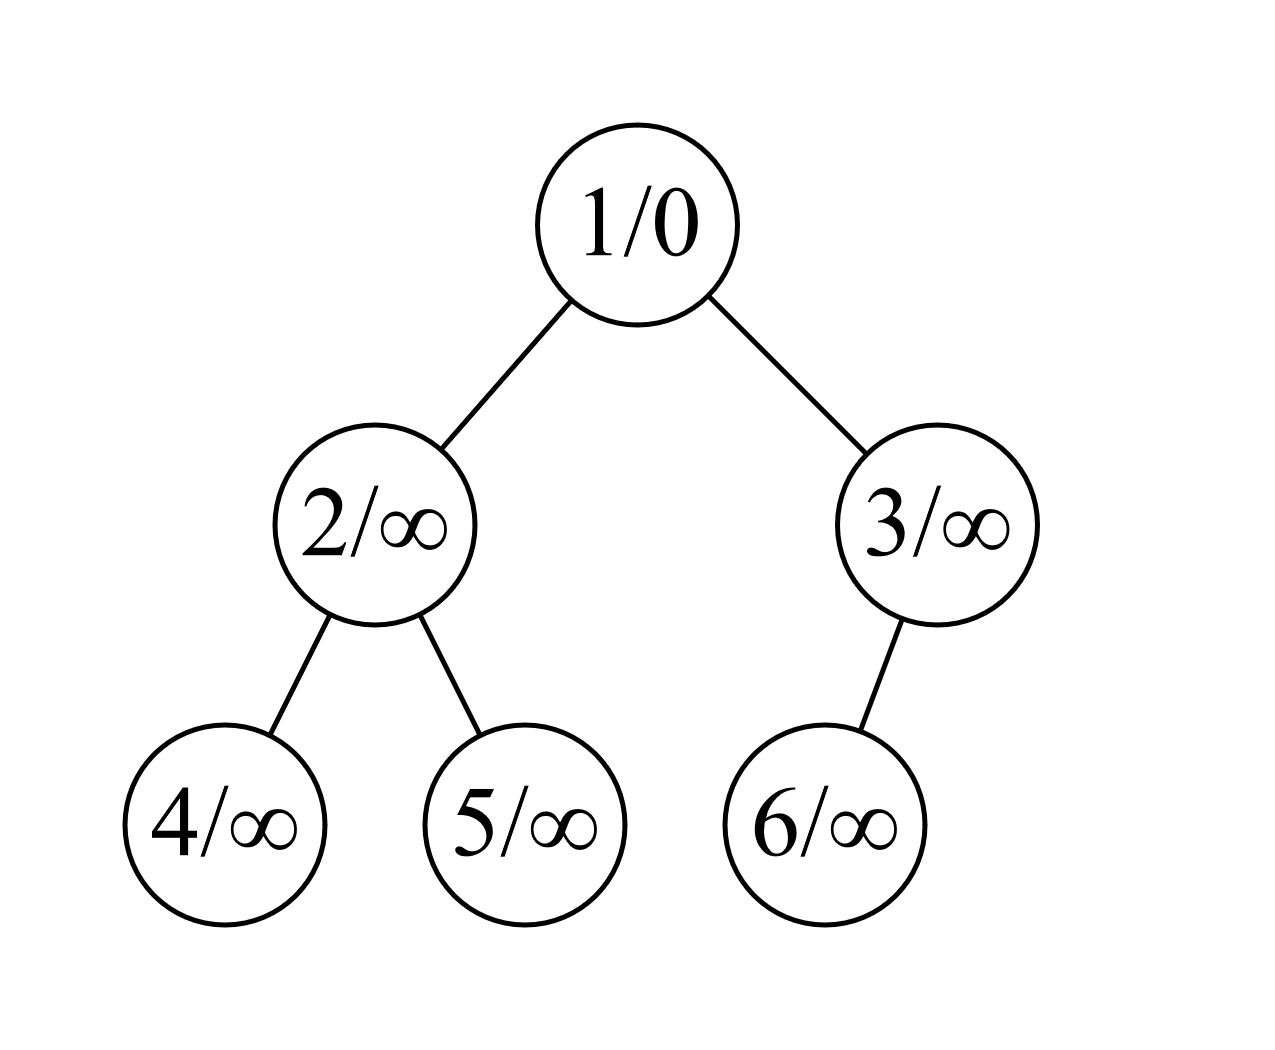
\includegraphics[width=0.8\textwidth]{img/2b_1.png}
            \end{subfigure}
            \begin{subfigure}{0.3\textwidth}
                \begin{tabular}{|c|c|c|c|c|c|}
                    \hline
                    $1$ & $2$ & $3$ & $4$ & $5$ & $6$ \\
                    \hline
                    $-$ & $-$ & $-$ & $-$ & $-$ & $-$ \\
                    \hline
                \end{tabular}
            \end{subfigure}
        \end{figure}
        \begin{figure}[h!]
            \centering
            \begin{subfigure}{0.3\textwidth}
                \centering
                \begin{tikzpicture}[scale=0.15]
                    \tikzstyle{every node}+=[inner sep=0pt]
                    \fill [black] (20.9,-19.3) circle (3);
                    \draw [black] (20.9,-19.3) circle (3);
                    \draw [white] (20.9,-19.3) node {$1$};
                    \fill [gray!60] (34.9,-19.3) circle (3);
                    \draw [black] (34.9,-19.3) circle (3);
                    \draw (34.9,-19.3) node {$2$};
                    \draw [black] (21.1,-32.2) circle (3);
                    \draw (21.1,-32.2) node {$4$};
                    \draw [black] (48.6,-19.3) circle (3);
                    \draw (48.6,-19.3) node {$3$};
                    \draw [black] (48.6,-32.2) circle (3);
                    \draw (48.6,-32.2) node {$6$};
                    \draw [black] (34.9,-32.2) circle (3);
                    \draw (34.9,-32.2) node {$5$};
                    \draw [black, dashed] (23.9,-19.3) -- (31.9,-19.3);
                    \draw (27.9,-18.8) node [above] {$1$};
                    \draw [black] (20.95,-22.3) -- (21.05,-29.2);
                    \draw (20.48,-25.75) node [left] {$1$};
                    \draw [black] (48.6,-22.3) -- (48.6,-29.2);
                    \draw (48.1,-25.75) node [left] {$2$};
                    \draw [black] (32.71,-21.35) -- (23.29,-30.15);
                    \draw (26.98,-25.27) node [above] {$2$};
                    \draw [black] (37.08,-21.36) -- (46.42,-30.14);
                    \draw (42.77,-25.27) node [above] {$3$};
                    \draw [black] (24.1,-32.2) -- (31.9,-32.2);
                    \draw (28,-31.7) node [above] {$3$};
                    \draw [black] (34.9,-29.2) -- (34.9,-22.3);
                    \draw (35.4,-25.75) node [right] {$4$};
                    \draw [black] (37.9,-19.3) -- (45.6,-19.3);
                    \draw (41.75,-18.8) node [above] {$4$};
                    \draw [black] (37.9,-32.2) -- (45.6,-32.2);
                    \draw (41.75,-31.7) node [above] {$4$};
                \end{tikzpicture}
            \end{subfigure}
            \begin{subfigure}{0.3\textwidth}
                \centering
                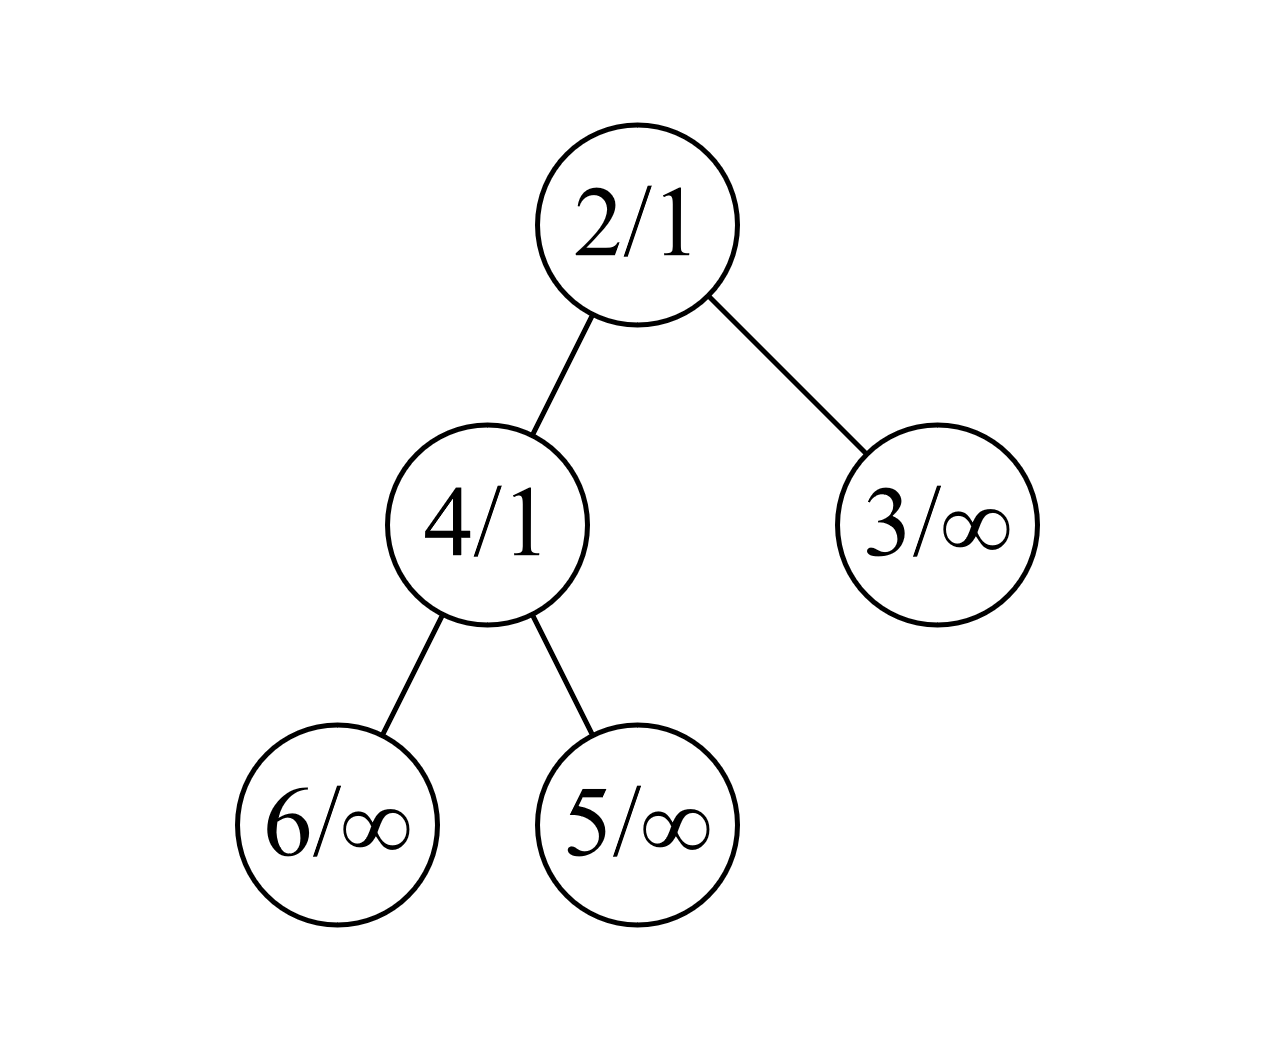
\includegraphics[width=0.8\textwidth]{img/2b_2.png}
            \end{subfigure}
            \begin{subfigure}{0.3\textwidth}
                \begin{tabular}{|c|c|c|c|c|c|}
                    \hline
                    $1$ & $2$ & $3$ & $4$ & $5$ & $6$ \\
                    \hline
                    $-$ & $1$ & $-$ & $1$ & $-$ & $-$ \\
                    \hline
                \end{tabular}
            \end{subfigure}
        \end{figure}
        \begin{figure}[h!]
            \centering
            \begin{subfigure}{0.3\textwidth}
                \centering
                \begin{tikzpicture}[scale=0.15]
                    \tikzstyle{every node}+=[inner sep=0pt]
                    \fill [black] (20.9,-19.3) circle (3);
                    \draw [black] (20.9,-19.3) circle (3);
                    \draw [white] (20.9,-19.3) node {$1$};
                    \fill [black] (34.9,-19.3) circle (3);
                    \draw [black] (34.9,-19.3) circle (3);
                    \draw [white] (34.9,-19.3) node {$2$};
                    \fill [gray!60] (21.1,-32.2) circle (3);
                    \draw [black] (21.1,-32.2) circle (3);
                    \draw (21.1,-32.2) node {$4$};
                    \draw [black] (48.6,-19.3) circle (3);
                    \draw (48.6,-19.3) node {$3$};
                    \draw [black] (48.6,-32.2) circle (3);
                    \draw (48.6,-32.2) node {$6$};
                    \draw [black] (34.9,-32.2) circle (3);
                    \draw (34.9,-32.2) node {$5$};
                    \draw [black, dashed] (23.9,-19.3) -- (31.9,-19.3);
                    \draw (27.9,-18.8) node [above] {$1$};
                    \draw [black, dashed] (20.95,-22.3) -- (21.05,-29.2);
                    \draw (20.48,-25.75) node [left] {$1$};
                    \draw [black] (48.6,-22.3) -- (48.6,-29.2);
                    \draw (48.1,-25.75) node [left] {$2$};
                    \draw [black] (32.71,-21.35) -- (23.29,-30.15);
                    \draw (26.98,-25.27) node [above] {$2$};
                    \draw [black] (37.08,-21.36) -- (46.42,-30.14);
                    \draw (42.77,-25.27) node [above] {$3$};
                    \draw [black] (24.1,-32.2) -- (31.9,-32.2);
                    \draw (28,-31.7) node [above] {$3$};
                    \draw [black] (34.9,-29.2) -- (34.9,-22.3);
                    \draw (35.4,-25.75) node [right] {$4$};
                    \draw [black] (37.9,-19.3) -- (45.6,-19.3);
                    \draw (41.75,-18.8) node [above] {$4$};
                    \draw [black] (37.9,-32.2) -- (45.6,-32.2);
                    \draw (41.75,-31.7) node [above] {$4$};
                \end{tikzpicture}
            \end{subfigure}
            \begin{subfigure}{0.3\textwidth}
                \centering
                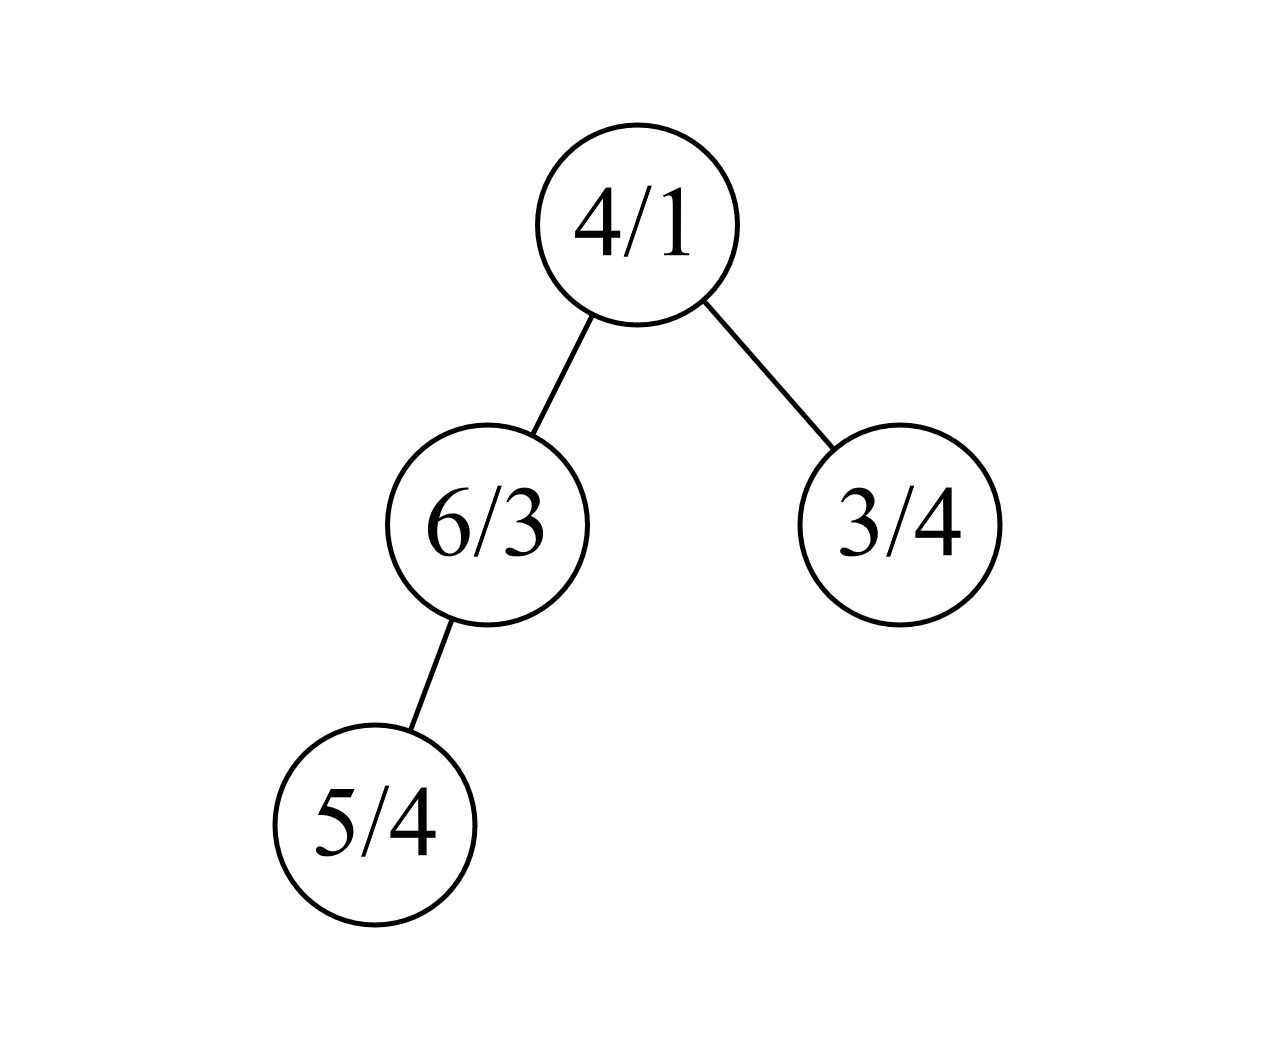
\includegraphics[width=0.8\textwidth]{img/2b_3.png}
            \end{subfigure}
            \begin{subfigure}{0.3\textwidth}
                \begin{tabular}{|c|c|c|c|c|c|}
                    \hline
                    $1$ & $2$ & $3$ & $4$ & $5$ & $6$ \\
                    \hline
                    $-$ & $1$ & $2$ & $1$ & $-$ & $2$ \\
                    \hline
                \end{tabular}
            \end{subfigure}
        \end{figure}
        \begin{figure}[h!]
            \centering
            \begin{subfigure}{0.3\textwidth}
                \centering
                \begin{tikzpicture}[scale=0.15]
                    \tikzstyle{every node}+=[inner sep=0pt]
                    \fill [black] (20.9,-19.3) circle (3);
                    \draw [black] (20.9,-19.3) circle (3);
                    \draw [white] (20.9,-19.3) node {$1$};
                    \fill [black] (34.9,-19.3) circle (3);
                    \draw [black] (34.9,-19.3) circle (3);
                    \draw [white] (34.9,-19.3) node {$2$};
                    \fill [black] (21.1,-32.2) circle (3);
                    \draw [black] (21.1,-32.2) circle (3);
                    \draw [white] (21.1,-32.2) node {$4$};
                    \draw [black] (48.6,-19.3) circle (3);
                    \draw (48.6,-19.3) node {$3$};
                    \fill [gray!60] (48.6,-32.2) circle (3);
                    \draw [black] (48.6,-32.2) circle (3);
                    \draw (48.6,-32.2) node {$6$};
                    \draw [black] (34.9,-32.2) circle (3);
                    \draw (34.9,-32.2) node {$5$};
                    \draw [black, dashed] (23.9,-19.3) -- (31.9,-19.3);
                    \draw (27.9,-18.8) node [above] {$1$};
                    \draw [black, dashed] (20.95,-22.3) -- (21.05,-29.2);
                    \draw (20.48,-25.75) node [left] {$1$};
                    \draw [black] (48.6,-22.3) -- (48.6,-29.2);
                    \draw (48.1,-25.75) node [left] {$2$};
                    \draw [black] (32.71,-21.35) -- (23.29,-30.15);
                    \draw (26.98,-25.27) node [above] {$2$};
                    \draw [black, dashed] (37.08,-21.36) -- (46.42,-30.14);
                    \draw (42.77,-25.27) node [above] {$3$};
                    \draw [black] (24.1,-32.2) -- (31.9,-32.2);
                    \draw (28,-31.7) node [above] {$3$};
                    \draw [black] (34.9,-29.2) -- (34.9,-22.3);
                    \draw (35.4,-25.75) node [right] {$4$};
                    \draw [black] (37.9,-19.3) -- (45.6,-19.3);
                    \draw (41.75,-18.8) node [above] {$4$};
                    \draw [black] (37.9,-32.2) -- (45.6,-32.2);
                    \draw (41.75,-31.7) node [above] {$4$};
                \end{tikzpicture}
            \end{subfigure}
            \begin{subfigure}{0.3\textwidth}
                \centering
                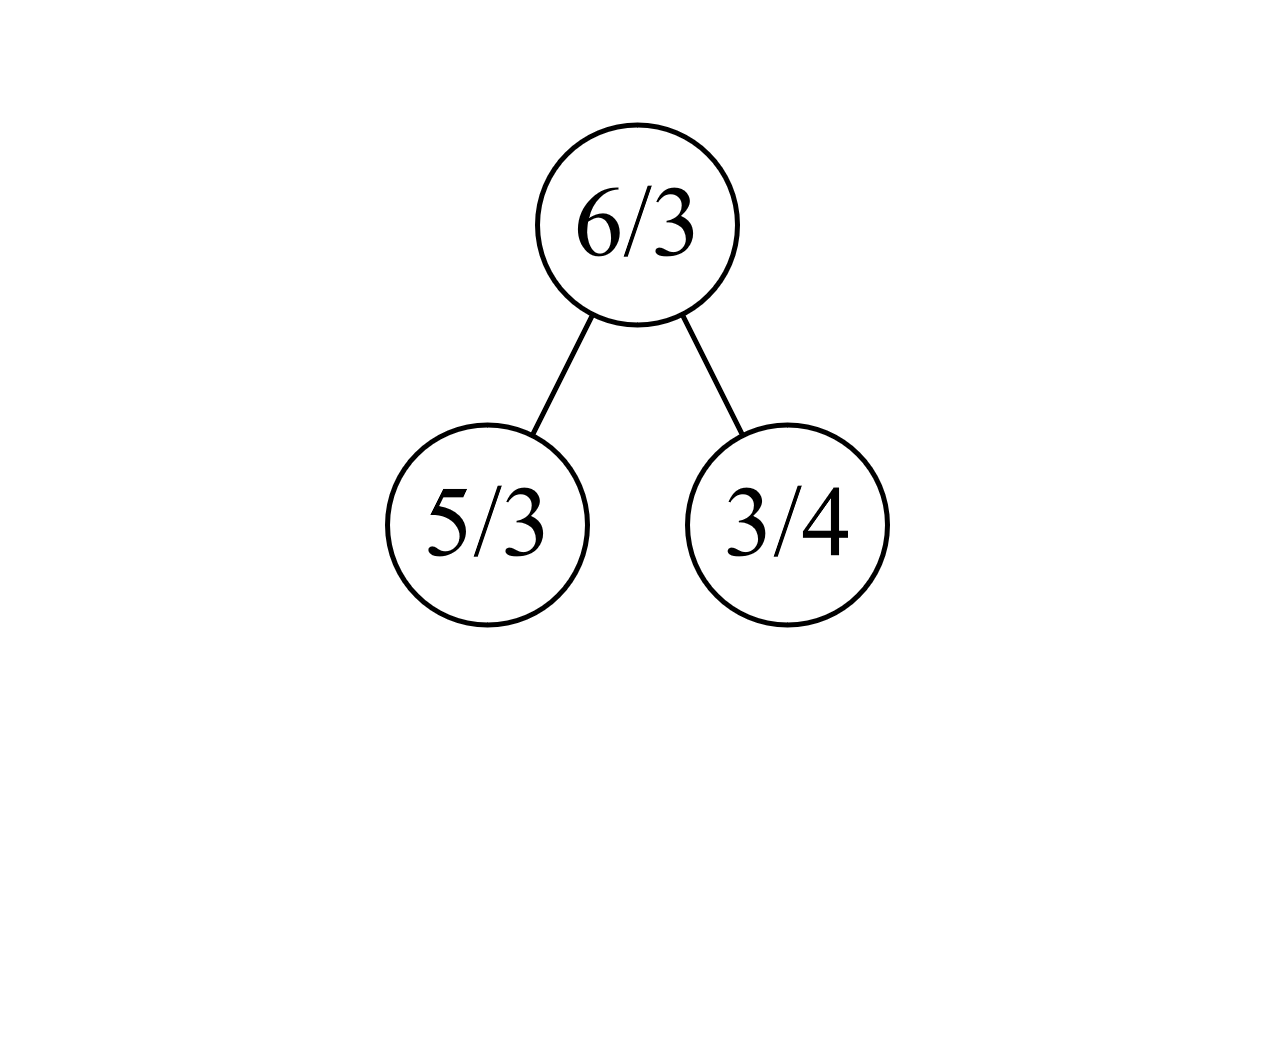
\includegraphics[width=0.8\textwidth]{img/2b_4.png}
            \end{subfigure}
            \begin{subfigure}{0.3\textwidth}
                \begin{tabular}{|c|c|c|c|c|c|}
                    \hline
                    $1$ & $2$ & $3$ & $4$ & $5$ & $6$ \\
                    \hline
                    $-$ & $1$ & $2$ & $1$ & $4$ & $2$ \\
                    \hline
                \end{tabular}
            \end{subfigure}
        \end{figure}
        \begin{figure}[h!]
            \centering
            \begin{subfigure}{0.3\textwidth}
                \centering
                \begin{tikzpicture}[scale=0.15]
                    \tikzstyle{every node}+=[inner sep=0pt]
                    \fill [black] (20.9,-19.3) circle (3);
                    \draw [black] (20.9,-19.3) circle (3);
                    \draw [white] (20.9,-19.3) node {$1$};
                    \fill [black] (34.9,-19.3) circle (3);
                    \draw [black] (34.9,-19.3) circle (3);
                    \draw [white] (34.9,-19.3) node {$2$};
                    \fill [black] (21.1,-32.2) circle (3);
                    \draw [black] (21.1,-32.2) circle (3);
                    \draw [white] (21.1,-32.2) node {$4$};
                    \fill [gray!60] (48.6,-19.3) circle (3);
                    \draw [black] (48.6,-19.3) circle (3);
                    \draw (48.6,-19.3) node {$3$};
                    \fill [black] (48.6,-32.2) circle (3);
                    \draw [black] (48.6,-32.2) circle (3);
                    \draw [white] (48.6,-32.2) node {$6$};
                    \draw [black] (34.9,-32.2) circle (3);
                    \draw (34.9,-32.2) node {$5$};
                    \draw [black, dashed] (23.9,-19.3) -- (31.9,-19.3);
                    \draw (27.9,-18.8) node [above] {$1$};
                    \draw [black, dashed] (20.95,-22.3) -- (21.05,-29.2);
                    \draw (20.48,-25.75) node [left] {$1$};
                    \draw [black, dashed] (48.6,-22.3) -- (48.6,-29.2);
                    \draw (48.1,-25.75) node [left] {$2$};
                    \draw [black] (32.71,-21.35) -- (23.29,-30.15);
                    \draw (26.98,-25.27) node [above] {$2$};
                    \draw [black, dashed] (37.08,-21.36) -- (46.42,-30.14);
                    \draw (42.77,-25.27) node [above] {$3$};
                    \draw [black] (24.1,-32.2) -- (31.9,-32.2);
                    \draw (28,-31.7) node [above] {$3$};
                    \draw [black] (34.9,-29.2) -- (34.9,-22.3);
                    \draw (35.4,-25.75) node [right] {$4$};
                    \draw [black] (37.9,-19.3) -- (45.6,-19.3);
                    \draw (41.75,-18.8) node [above] {$4$};
                    \draw [black] (37.9,-32.2) -- (45.6,-32.2);
                    \draw (41.75,-31.7) node [above] {$4$};
                \end{tikzpicture}
            \end{subfigure}
            \begin{subfigure}{0.3\textwidth}
                \centering
                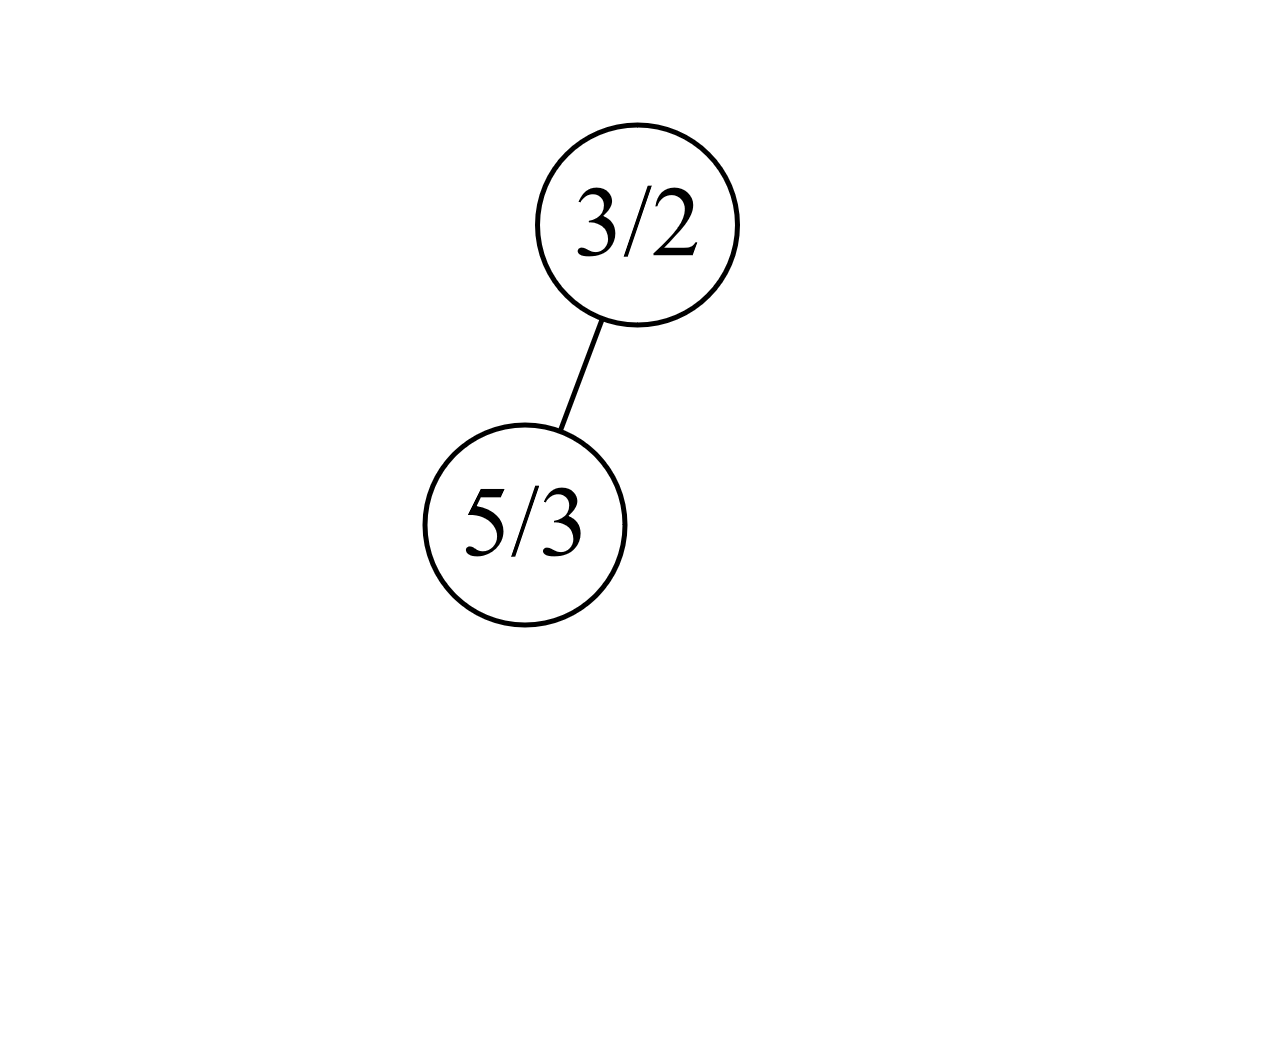
\includegraphics[width=0.8\textwidth]{img/2b_5.png}
            \end{subfigure}
            \begin{subfigure}{0.3\textwidth}
                \begin{tabular}{|c|c|c|c|c|c|}
                    \hline
                    $1$ & $2$ & $3$ & $4$ & $5$ & $6$ \\
                    \hline
                    $-$ & $1$ & $6$ & $1$ & $4$ & $2$ \\
                    \hline
                \end{tabular}
            \end{subfigure}
        \end{figure}
        \begin{figure}[h!]
            \centering
            \begin{subfigure}{0.3\textwidth}
                \centering
                \begin{tikzpicture}[scale=0.15]
                    \tikzstyle{every node}+=[inner sep=0pt]
                    \fill [black] (20.9,-19.3) circle (3);
                    \draw [black] (20.9,-19.3) circle (3);
                    \draw [white] (20.9,-19.3) node {$1$};
                    \fill [black] (34.9,-19.3) circle (3);
                    \draw [black] (34.9,-19.3) circle (3);
                    \draw [white] (34.9,-19.3) node {$2$};
                    \fill [black] (21.1,-32.2) circle (3);
                    \draw [black] (21.1,-32.2) circle (3);
                    \draw [white] (21.1,-32.2) node {$4$};
                    \fill [black] (48.6,-19.3) circle (3);
                    \draw [black] (48.6,-19.3) circle (3);
                    \draw [white] (48.6,-19.3) node {$3$};
                    \fill [black] (48.6,-32.2) circle (3);
                    \draw [black] (48.6,-32.2) circle (3);
                    \draw [white] (48.6,-32.2) node {$6$};
                    \fill [gray!60] (34.9,-32.2) circle (3);
                    \draw [black] (34.9,-32.2) circle (3);
                    \draw (34.9,-32.2) node {$5$};
                    \draw [black, dashed] (23.9,-19.3) -- (31.9,-19.3);
                    \draw (27.9,-18.8) node [above] {$1$};
                    \draw [black, dashed] (20.95,-22.3) -- (21.05,-29.2);
                    \draw (20.48,-25.75) node [left] {$1$};
                    \draw [black, dashed] (48.6,-22.3) -- (48.6,-29.2);
                    \draw (48.1,-25.75) node [left] {$2$};
                    \draw [black] (32.71,-21.35) -- (23.29,-30.15);
                    \draw (26.98,-25.27) node [above] {$2$};
                    \draw [black, dashed] (37.08,-21.36) -- (46.42,-30.14);
                    \draw (42.77,-25.27) node [above] {$3$};
                    \draw [black, dashed] (24.1,-32.2) -- (31.9,-32.2);
                    \draw (28,-31.7) node [above] {$3$};
                    \draw [black] (34.9,-29.2) -- (34.9,-22.3);
                    \draw (35.4,-25.75) node [right] {$4$};
                    \draw [black] (37.9,-19.3) -- (45.6,-19.3);
                    \draw (41.75,-18.8) node [above] {$4$};
                    \draw [black] (37.9,-32.2) -- (45.6,-32.2);
                    \draw (41.75,-31.7) node [above] {$4$};
                \end{tikzpicture}
            \end{subfigure}
            \begin{subfigure}{0.3\textwidth}
                \centering
                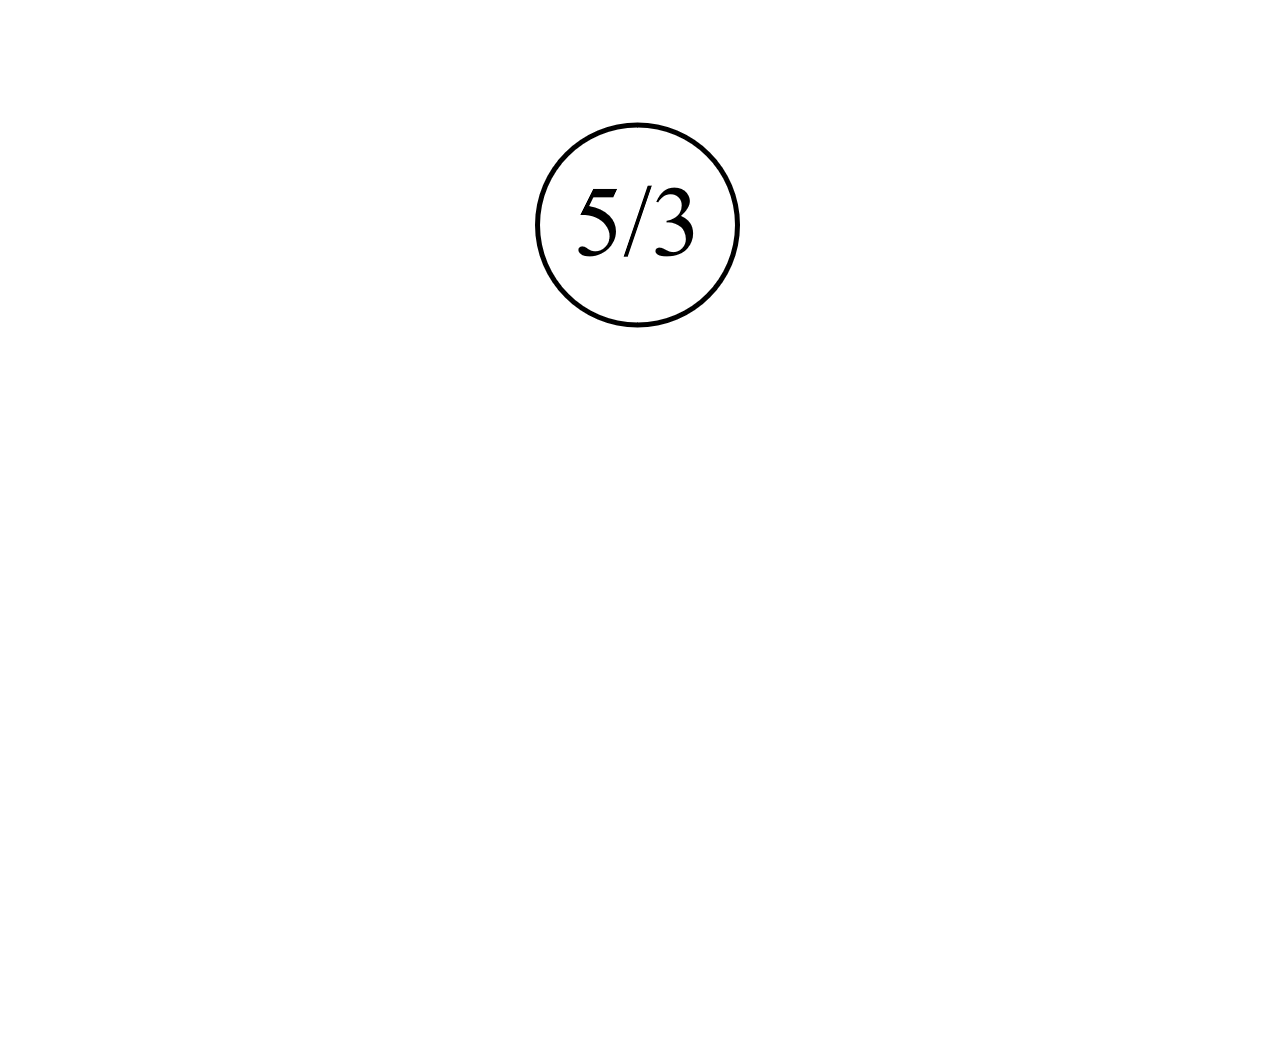
\includegraphics[width=0.8\textwidth]{img/2b_6.png}
            \end{subfigure}
            \begin{subfigure}{0.3\textwidth}
                \begin{tabular}{|c|c|c|c|c|c|}
                    \hline
                    $1$ & $2$ & $3$ & $4$ & $5$ & $6$ \\
                    \hline
                    $-$ & $1$ & $6$ & $1$ & $4$ & $2$ \\
                    \hline
                \end{tabular}
            \end{subfigure}
        \end{figure}
        \FloatBarrier
        $G_2$:
        \begin{figure}[h!]
            \centering
            \begin{tikzpicture}[scale=0.13]
                \tikzstyle{every node}+=[inner sep=0pt]
                \fill [gray!60] (16.1,-16.8) circle (3);
                \draw [black] (16.1,-16.8) circle (3);
                \draw (16.1,-16.8) node {$1$};
                \draw [black] (32.1,-16.8) circle (3);
                \draw (32.1,-16.8) node {$2$};
                \draw [black] (16.1,-31.8) circle (3);
                \draw (16.1,-31.8) node {$4$};
                \draw [black] (32.1,-31.8) circle (3);
                \draw (32.1,-31.8) node {$5$};
                \draw [black] (47.8,-31.8) circle (3);
                \draw (47.8,-31.8) node {$6$};
                \draw [black] (47.8,-16.8) circle (3);
                \draw (47.8,-16.8) node {$3$};
                \draw [black] (16.1,-47.2) circle (3);
                \draw (16.1,-47.2) node {$7$};
                \draw [black] (32.1,-47.2) circle (3);
                \draw (32.1,-47.2) node {$8$};
                \draw [black] (47.8,-47.2) circle (3);
                \draw (47.8,-47.2) node {$9$};
                \draw [black] (34.27,-29.73) -- (45.63,-18.87);
                \draw (38.93,-23.82) node [above] {$1$};
                \draw [black] (44.8,-31.8) -- (35.1,-31.8);
                \draw (39.95,-31.3) node [above] {$2$};
                \draw [black] (47.8,-28.8) -- (47.8,-19.8);
                \draw (47.3,-24.3) node [left] {$3$};
                \draw [black] (19.1,-47.2) -- (29.1,-47.2);
                \draw (24.1,-46.7) node [above] {$4$};
                \draw [black] (18.29,-29.75) -- (29.91,-18.85);
                \draw (23.08,-23.82) node [above] {$5$};
                \draw [black] (19.1,-31.8) -- (29.1,-31.8);
                \draw (24.1,-31.3) node [above] {$6$};
                \draw [black] (16.1,-34.8) -- (16.1,-44.2);
                \draw (15.6,-39.5) node [left] {$7$};
                \draw [black] (32.1,-34.8) -- (32.1,-44.2);
                \draw (31.6,-39.5) node [left] {$8$};
                \draw [black] (35.1,-16.8) -- (44.8,-16.8);
                \draw (39.95,-16.3) node [above] {$9$};
                \draw [black] (19.1,-16.8) -- (29.1,-16.8);
                \draw (24.1,-16.3) node [above] {$10$};
                \draw [black] (16.1,-19.8) -- (16.1,-28.8);
                \draw (15.6,-24.3) node [left] {$11$};
                \draw [black] (47.8,-34.8) -- (47.8,-44.2);
                \draw (47.3,-39.5) node [left] {$13$};
                \draw [black] (35.1,-47.2) -- (44.8,-47.2);
                \draw (39.95,-46.7) node [above] {$14$};
                \draw [black] (34.24,-45.1) -- (45.66,-33.9);
                \draw (38.43,-39.02) node [above] {$12$};
                \draw [black] (18.26,-45.12) -- (29.94,-33.88);
                \draw (22.58,-39.02) node [above] {$15$};
                \draw [black] (32.1,-28.8) -- (32.1,-19.8);
                \draw (31.6,-24.3) node [left] {$16$};
            \end{tikzpicture}
        \end{figure}
        \begin{figure}[h!]
            \centering
            \begin{tikzpicture}[scale=0.13]
                \tikzstyle{every node}+=[inner sep=0pt]
                \fill [black] (16.1,-16.8) circle (3);
                \draw [black] (16.1,-16.8) circle (3);
                \draw [white] (16.1,-16.8) node {$1$};
                \fill [gray!60] (32.1,-16.8) circle (3);
                \draw [black] (32.1,-16.8) circle (3);
                \draw (32.1,-16.8) node {$2$};
                \draw [black] (16.1,-31.8) circle (3);
                \draw (16.1,-31.8) node {$4$};
                \draw [black] (32.1,-31.8) circle (3);
                \draw (32.1,-31.8) node {$5$};
                \draw [black] (47.8,-31.8) circle (3);
                \draw (47.8,-31.8) node {$6$};
                \draw [black] (47.8,-16.8) circle (3);
                \draw (47.8,-16.8) node {$3$};
                \draw [black] (16.1,-47.2) circle (3);
                \draw (16.1,-47.2) node {$7$};
                \draw [black] (32.1,-47.2) circle (3);
                \draw (32.1,-47.2) node {$8$};
                \draw [black] (47.8,-47.2) circle (3);
                \draw (47.8,-47.2) node {$9$};
                \draw [black] (34.27,-29.73) -- (45.63,-18.87);
                \draw (38.93,-23.82) node [above] {$1$};
                \draw [black] (44.8,-31.8) -- (35.1,-31.8);
                \draw (39.95,-31.3) node [above] {$2$};
                \draw [black] (47.8,-28.8) -- (47.8,-19.8);
                \draw (47.3,-24.3) node [left] {$3$};
                \draw [black] (19.1,-47.2) -- (29.1,-47.2);
                \draw (24.1,-46.7) node [above] {$4$};
                \draw [black] (18.29,-29.75) -- (29.91,-18.85);
                \draw (23.08,-23.82) node [above] {$5$};
                \draw [black] (19.1,-31.8) -- (29.1,-31.8);
                \draw (24.1,-31.3) node [above] {$6$};
                \draw [black] (16.1,-34.8) -- (16.1,-44.2);
                \draw (15.6,-39.5) node [left] {$7$};
                \draw [black] (32.1,-34.8) -- (32.1,-44.2);
                \draw (31.6,-39.5) node [left] {$8$};
                \draw [black] (35.1,-16.8) -- (44.8,-16.8);
                \draw (39.95,-16.3) node [above] {$9$};
                \draw [black, dashed] (19.1,-16.8) -- (29.1,-16.8);
                \draw (24.1,-16.3) node [above] {$10$};
                \draw [black] (16.1,-19.8) -- (16.1,-28.8);
                \draw (15.6,-24.3) node [left] {$11$};
                \draw [black] (47.8,-34.8) -- (47.8,-44.2);
                \draw (47.3,-39.5) node [left] {$13$};
                \draw [black] (35.1,-47.2) -- (44.8,-47.2);
                \draw (39.95,-46.7) node [above] {$14$};
                \draw [black] (34.24,-45.1) -- (45.66,-33.9);
                \draw (38.43,-39.02) node [above] {$12$};
                \draw [black] (18.26,-45.12) -- (29.94,-33.88);
                \draw (22.58,-39.02) node [above] {$15$};
                \draw [black] (32.1,-28.8) -- (32.1,-19.8);
                \draw (31.6,-24.3) node [left] {$16$};
            \end{tikzpicture}
        \end{figure}
        \begin{figure}[h!]
            \centering
            \begin{tikzpicture}[scale=0.13]
                \tikzstyle{every node}+=[inner sep=0pt]
                \fill [black] (16.1,-16.8) circle (3);
                \draw [black] (16.1,-16.8) circle (3);
                \draw [white] (16.1,-16.8) node {$1$};
                \fill [black] (32.1,-16.8) circle (3);
                \draw [black] (32.1,-16.8) circle (3);
                \draw [white] (32.1,-16.8) node {$2$};
                \fill [gray!60] (16.1,-31.8) circle (3);
                \draw [black] (16.1,-31.8) circle (3);
                \draw (16.1,-31.8) node {$4$};
                \draw [black] (32.1,-31.8) circle (3);
                \draw (32.1,-31.8) node {$5$};
                \draw [black] (47.8,-31.8) circle (3);
                \draw (47.8,-31.8) node {$6$};
                \draw [black] (47.8,-16.8) circle (3);
                \draw (47.8,-16.8) node {$3$};
                \draw [black] (16.1,-47.2) circle (3);
                \draw (16.1,-47.2) node {$7$};
                \draw [black] (32.1,-47.2) circle (3);
                \draw (32.1,-47.2) node {$8$};
                \draw [black] (47.8,-47.2) circle (3);
                \draw (47.8,-47.2) node {$9$};
                \draw [black] (34.27,-29.73) -- (45.63,-18.87);
                \draw (38.93,-23.82) node [above] {$1$};
                \draw [black] (44.8,-31.8) -- (35.1,-31.8);
                \draw (39.95,-31.3) node [above] {$2$};
                \draw [black] (47.8,-28.8) -- (47.8,-19.8);
                \draw (47.3,-24.3) node [left] {$3$};
                \draw [black] (19.1,-47.2) -- (29.1,-47.2);
                \draw (24.1,-46.7) node [above] {$4$};
                \draw [black, dashed] (18.29,-29.75) -- (29.91,-18.85);
                \draw (23.08,-23.82) node [above] {$5$};
                \draw [black] (19.1,-31.8) -- (29.1,-31.8);
                \draw (24.1,-31.3) node [above] {$6$};
                \draw [black] (16.1,-34.8) -- (16.1,-44.2);
                \draw (15.6,-39.5) node [left] {$7$};
                \draw [black] (32.1,-34.8) -- (32.1,-44.2);
                \draw (31.6,-39.5) node [left] {$8$};
                \draw [black] (35.1,-16.8) -- (44.8,-16.8);
                \draw (39.95,-16.3) node [above] {$9$};
                \draw [black, dashed] (19.1,-16.8) -- (29.1,-16.8);
                \draw (24.1,-16.3) node [above] {$10$};
                \draw [black] (16.1,-19.8) -- (16.1,-28.8);
                \draw (15.6,-24.3) node [left] {$11$};
                \draw [black] (47.8,-34.8) -- (47.8,-44.2);
                \draw (47.3,-39.5) node [left] {$13$};
                \draw [black] (35.1,-47.2) -- (44.8,-47.2);
                \draw (39.95,-46.7) node [above] {$14$};
                \draw [black] (34.24,-45.1) -- (45.66,-33.9);
                \draw (38.43,-39.02) node [above] {$12$};
                \draw [black] (18.26,-45.12) -- (29.94,-33.88);
                \draw (22.58,-39.02) node [above] {$15$};
                \draw [black] (32.1,-28.8) -- (32.1,-19.8);
                \draw (31.6,-24.3) node [left] {$16$};
            \end{tikzpicture}
        \end{figure}
        \begin{figure}[h!]
            \centering
            \begin{tikzpicture}[scale=0.13]
                \tikzstyle{every node}+=[inner sep=0pt]
                \fill [black] (16.1,-16.8) circle (3);
                \draw [black] (16.1,-16.8) circle (3);
                \draw [white] (16.1,-16.8) node {$1$};
                \fill [black] (32.1,-16.8) circle (3);
                \draw [black] (32.1,-16.8) circle (3);
                \draw [white] (32.1,-16.8) node {$2$};
                \fill [black] (16.1,-31.8) circle (3);
                \draw [black] (16.1,-31.8) circle (3);
                \draw [white] (16.1,-31.8) node {$4$};
                \fill [gray!60] (32.1,-31.8) circle (3);
                \draw [black] (32.1,-31.8) circle (3);
                \draw (32.1,-31.8) node {$5$};
                \draw [black] (47.8,-31.8) circle (3);
                \draw (47.8,-31.8) node {$6$};
                \draw [black] (47.8,-16.8) circle (3);
                \draw (47.8,-16.8) node {$3$};
                \draw [black] (16.1,-47.2) circle (3);
                \draw (16.1,-47.2) node {$7$};
                \draw [black] (32.1,-47.2) circle (3);
                \draw (32.1,-47.2) node {$8$};
                \draw [black] (47.8,-47.2) circle (3);
                \draw (47.8,-47.2) node {$9$};
                \draw [black] (34.27,-29.73) -- (45.63,-18.87);
                \draw (38.93,-23.82) node [above] {$1$};
                \draw [black] (44.8,-31.8) -- (35.1,-31.8);
                \draw (39.95,-31.3) node [above] {$2$};
                \draw [black] (47.8,-28.8) -- (47.8,-19.8);
                \draw (47.3,-24.3) node [left] {$3$};
                \draw [black] (19.1,-47.2) -- (29.1,-47.2);
                \draw (24.1,-46.7) node [above] {$4$};
                \draw [black, dashed] (18.29,-29.75) -- (29.91,-18.85);
                \draw (23.08,-23.82) node [above] {$5$};
                \draw [black, dashed] (19.1,-31.8) -- (29.1,-31.8);
                \draw (24.1,-31.3) node [above] {$6$};
                \draw [black] (16.1,-34.8) -- (16.1,-44.2);
                \draw (15.6,-39.5) node [left] {$7$};
                \draw [black] (32.1,-34.8) -- (32.1,-44.2);
                \draw (31.6,-39.5) node [left] {$8$};
                \draw [black] (35.1,-16.8) -- (44.8,-16.8);
                \draw (39.95,-16.3) node [above] {$9$};
                \draw [black, dashed] (19.1,-16.8) -- (29.1,-16.8);
                \draw (24.1,-16.3) node [above] {$10$};
                \draw [black] (16.1,-19.8) -- (16.1,-28.8);
                \draw (15.6,-24.3) node [left] {$11$};
                \draw [black] (47.8,-34.8) -- (47.8,-44.2);
                \draw (47.3,-39.5) node [left] {$13$};
                \draw [black] (35.1,-47.2) -- (44.8,-47.2);
                \draw (39.95,-46.7) node [above] {$14$};
                \draw [black] (34.24,-45.1) -- (45.66,-33.9);
                \draw (38.43,-39.02) node [above] {$12$};
                \draw [black] (18.26,-45.12) -- (29.94,-33.88);
                \draw (22.58,-39.02) node [above] {$15$};
                \draw [black] (32.1,-28.8) -- (32.1,-19.8);
                \draw (31.6,-24.3) node [left] {$16$};
            \end{tikzpicture}
        \end{figure}
        \begin{figure}[h!]
            \centering
            \begin{tikzpicture}[scale=0.13]
                \tikzstyle{every node}+=[inner sep=0pt]
                \fill [black] (16.1,-16.8) circle (3);
                \draw [black] (16.1,-16.8) circle (3);
                \draw [white] (16.1,-16.8) node {$1$};
                \fill [black] (32.1,-16.8) circle (3);
                \draw [black] (32.1,-16.8) circle (3);
                \draw [white] (32.1,-16.8) node {$2$};
                \fill [black] (16.1,-31.8) circle (3);
                \draw [black] (16.1,-31.8) circle (3);
                \draw [white] (16.1,-31.8) node {$4$};
                \fill [black] (32.1,-31.8) circle (3);
                \draw [black] (32.1,-31.8) circle (3);
                \draw [white] (32.1,-31.8) node {$5$};
                \draw [black] (47.8,-31.8) circle (3);
                \draw (47.8,-31.8) node {$6$};
                \fill [gray!60] (47.8,-16.8) circle (3);
                \draw [black] (47.8,-16.8) circle (3);
                \draw (47.8,-16.8) node {$3$};
                \draw [black] (16.1,-47.2) circle (3);
                \draw (16.1,-47.2) node {$7$};
                \draw [black] (32.1,-47.2) circle (3);
                \draw (32.1,-47.2) node {$8$};
                \draw [black] (47.8,-47.2) circle (3);
                \draw (47.8,-47.2) node {$9$};
                \draw [black, dashed] (34.27,-29.73) -- (45.63,-18.87);
                \draw (38.93,-23.82) node [above] {$1$};
                \draw [black] (44.8,-31.8) -- (35.1,-31.8);
                \draw (39.95,-31.3) node [above] {$2$};
                \draw [black] (47.8,-28.8) -- (47.8,-19.8);
                \draw (47.3,-24.3) node [left] {$3$};
                \draw [black] (19.1,-47.2) -- (29.1,-47.2);
                \draw (24.1,-46.7) node [above] {$4$};
                \draw [black, dashed] (18.29,-29.75) -- (29.91,-18.85);
                \draw (23.08,-23.82) node [above] {$5$};
                \draw [black, dashed] (19.1,-31.8) -- (29.1,-31.8);
                \draw (24.1,-31.3) node [above] {$6$};
                \draw [black] (16.1,-34.8) -- (16.1,-44.2);
                \draw (15.6,-39.5) node [left] {$7$};
                \draw [black] (32.1,-34.8) -- (32.1,-44.2);
                \draw (31.6,-39.5) node [left] {$8$};
                \draw [black] (35.1,-16.8) -- (44.8,-16.8);
                \draw (39.95,-16.3) node [above] {$9$};
                \draw [black, dashed] (19.1,-16.8) -- (29.1,-16.8);
                \draw (24.1,-16.3) node [above] {$10$};
                \draw [black] (16.1,-19.8) -- (16.1,-28.8);
                \draw (15.6,-24.3) node [left] {$11$};
                \draw [black] (47.8,-34.8) -- (47.8,-44.2);
                \draw (47.3,-39.5) node [left] {$13$};
                \draw [black] (35.1,-47.2) -- (44.8,-47.2);
                \draw (39.95,-46.7) node [above] {$14$};
                \draw [black] (34.24,-45.1) -- (45.66,-33.9);
                \draw (38.43,-39.02) node [above] {$12$};
                \draw [black] (18.26,-45.12) -- (29.94,-33.88);
                \draw (22.58,-39.02) node [above] {$15$};
                \draw [black] (32.1,-28.8) -- (32.1,-19.8);
                \draw (31.6,-24.3) node [left] {$16$};
            \end{tikzpicture}
        \end{figure}
        \begin{figure}[h!]
            \centering
            \begin{tikzpicture}[scale=0.13]
                \tikzstyle{every node}+=[inner sep=0pt]
                \fill [black] (16.1,-16.8) circle (3);
                \draw [black] (16.1,-16.8) circle (3);
                \draw [white] (16.1,-16.8) node {$1$};
                \fill [black] (32.1,-16.8) circle (3);
                \draw [black] (32.1,-16.8) circle (3);
                \draw [white] (32.1,-16.8) node {$2$};
                \fill [black] (16.1,-31.8) circle (3);
                \draw [black] (16.1,-31.8) circle (3);
                \draw [white] (16.1,-31.8) node {$4$};
                \fill [black] (32.1,-31.8) circle (3);
                \draw [black] (32.1,-31.8) circle (3);
                \draw [white] (32.1,-31.8) node {$5$};
                \fill [gray!60] (47.8,-31.8) circle (3);
                \draw [black] (47.8,-31.8) circle (3);
                \draw (47.8,-31.8) node {$6$};
                \fill [black] (47.8,-16.8) circle (3);
                \draw [black] (47.8,-16.8) circle (3);
                \draw [white] (47.8,-16.8) node {$3$};
                \draw [black] (16.1,-47.2) circle (3);
                \draw (16.1,-47.2) node {$7$};
                \draw [black] (32.1,-47.2) circle (3);
                \draw (32.1,-47.2) node {$8$};
                \draw [black] (47.8,-47.2) circle (3);
                \draw (47.8,-47.2) node {$9$};
                \draw [black, dashed] (34.27,-29.73) -- (45.63,-18.87);
                \draw (38.93,-23.82) node [above] {$1$};
                \draw [black, dashed] (44.8,-31.8) -- (35.1,-31.8);
                \draw (39.95,-31.3) node [above] {$2$};
                \draw [black] (47.8,-28.8) -- (47.8,-19.8);
                \draw (47.3,-24.3) node [left] {$3$};
                \draw [black] (19.1,-47.2) -- (29.1,-47.2);
                \draw (24.1,-46.7) node [above] {$4$};
                \draw [black, dashed] (18.29,-29.75) -- (29.91,-18.85);
                \draw (23.08,-23.82) node [above] {$5$};
                \draw [black, dashed] (19.1,-31.8) -- (29.1,-31.8);
                \draw (24.1,-31.3) node [above] {$6$};
                \draw [black] (16.1,-34.8) -- (16.1,-44.2);
                \draw (15.6,-39.5) node [left] {$7$};
                \draw [black] (32.1,-34.8) -- (32.1,-44.2);
                \draw (31.6,-39.5) node [left] {$8$};
                \draw [black] (35.1,-16.8) -- (44.8,-16.8);
                \draw (39.95,-16.3) node [above] {$9$};
                \draw [black, dashed] (19.1,-16.8) -- (29.1,-16.8);
                \draw (24.1,-16.3) node [above] {$10$};
                \draw [black] (16.1,-19.8) -- (16.1,-28.8);
                \draw (15.6,-24.3) node [left] {$11$};
                \draw [black] (47.8,-34.8) -- (47.8,-44.2);
                \draw (47.3,-39.5) node [left] {$13$};
                \draw [black] (35.1,-47.2) -- (44.8,-47.2);
                \draw (39.95,-46.7) node [above] {$14$};
                \draw [black] (34.24,-45.1) -- (45.66,-33.9);
                \draw (38.43,-39.02) node [above] {$12$};
                \draw [black] (18.26,-45.12) -- (29.94,-33.88);
                \draw (22.58,-39.02) node [above] {$15$};
                \draw [black] (32.1,-28.8) -- (32.1,-19.8);
                \draw (31.6,-24.3) node [left] {$16$};
            \end{tikzpicture}
        \end{figure}
        \begin{figure}[h!]
            \centering
            \begin{tikzpicture}[scale=0.13]
                \tikzstyle{every node}+=[inner sep=0pt]
                \fill [black] (16.1,-16.8) circle (3);
                \draw [black] (16.1,-16.8) circle (3);
                \draw [white] (16.1,-16.8) node {$1$};
                \fill [black] (32.1,-16.8) circle (3);
                \draw [black] (32.1,-16.8) circle (3);
                \draw [white] (32.1,-16.8) node {$2$};
                \fill [black] (16.1,-31.8) circle (3);
                \draw [black] (16.1,-31.8) circle (3);
                \draw [white] (16.1,-31.8) node {$4$};
                \fill [black] (32.1,-31.8) circle (3);
                \draw [black] (32.1,-31.8) circle (3);
                \draw [white] (32.1,-31.8) node {$5$};
                \fill [black] (47.8,-31.8) circle (3);
                \draw [black] (47.8,-31.8) circle (3);
                \draw [white] (47.8,-31.8) node {$6$};
                \fill [black] (47.8,-16.8) circle (3);
                \draw [black] (47.8,-16.8) circle (3);
                \draw [white] (47.8,-16.8) node {$3$};
                \fill [gray!60] (16.1,-47.2) circle (3);
                \draw [black] (16.1,-47.2) circle (3);
                \draw (16.1,-47.2) node {$7$};
                \draw [black] (32.1,-47.2) circle (3);
                \draw (32.1,-47.2) node {$8$};
                \draw [black] (47.8,-47.2) circle (3);
                \draw (47.8,-47.2) node {$9$};
                \draw [black, dashed] (34.27,-29.73) -- (45.63,-18.87);
                \draw (38.93,-23.82) node [above] {$1$};
                \draw [black, dashed] (44.8,-31.8) -- (35.1,-31.8);
                \draw (39.95,-31.3) node [above] {$2$};
                \draw [black] (47.8,-28.8) -- (47.8,-19.8);
                \draw (47.3,-24.3) node [left] {$3$};
                \draw [black] (19.1,-47.2) -- (29.1,-47.2);
                \draw (24.1,-46.7) node [above] {$4$};
                \draw [black, dashed] (18.29,-29.75) -- (29.91,-18.85);
                \draw (23.08,-23.82) node [above] {$5$};
                \draw [black, dashed] (19.1,-31.8) -- (29.1,-31.8);
                \draw (24.1,-31.3) node [above] {$6$};
                \draw [black, dashed] (16.1,-34.8) -- (16.1,-44.2);
                \draw (15.6,-39.5) node [left] {$7$};
                \draw [black] (32.1,-34.8) -- (32.1,-44.2);
                \draw (31.6,-39.5) node [left] {$8$};
                \draw [black] (35.1,-16.8) -- (44.8,-16.8);
                \draw (39.95,-16.3) node [above] {$9$};
                \draw [black, dashed] (19.1,-16.8) -- (29.1,-16.8);
                \draw (24.1,-16.3) node [above] {$10$};
                \draw [black] (16.1,-19.8) -- (16.1,-28.8);
                \draw (15.6,-24.3) node [left] {$11$};
                \draw [black] (47.8,-34.8) -- (47.8,-44.2);
                \draw (47.3,-39.5) node [left] {$13$};
                \draw [black] (35.1,-47.2) -- (44.8,-47.2);
                \draw (39.95,-46.7) node [above] {$14$};
                \draw [black] (34.24,-45.1) -- (45.66,-33.9);
                \draw (38.43,-39.02) node [above] {$12$};
                \draw [black] (18.26,-45.12) -- (29.94,-33.88);
                \draw (22.58,-39.02) node [above] {$15$};
                \draw [black] (32.1,-28.8) -- (32.1,-19.8);
                \draw (31.6,-24.3) node [left] {$16$};
            \end{tikzpicture}
        \end{figure}
        \begin{figure}[h!]
            \centering
            \begin{tikzpicture}[scale=0.13]
                \tikzstyle{every node}+=[inner sep=0pt]
                \fill [black] (16.1,-16.8) circle (3);
                \draw [black] (16.1,-16.8) circle (3);
                \draw [white] (16.1,-16.8) node {$1$};
                \fill [black] (32.1,-16.8) circle (3);
                \draw [black] (32.1,-16.8) circle (3);
                \draw [white] (32.1,-16.8) node {$2$};
                \fill [black] (16.1,-31.8) circle (3);
                \draw [black] (16.1,-31.8) circle (3);
                \draw [white] (16.1,-31.8) node {$4$};
                \fill [black] (32.1,-31.8) circle (3);
                \draw [black] (32.1,-31.8) circle (3);
                \draw [white] (32.1,-31.8) node {$5$};
                \fill [black] (47.8,-31.8) circle (3);
                \draw [black] (47.8,-31.8) circle (3);
                \draw [white] (47.8,-31.8) node {$6$};
                \fill [black] (47.8,-16.8) circle (3);
                \draw [black] (47.8,-16.8) circle (3);
                \draw [white] (47.8,-16.8) node {$3$};
                \fill [black] (16.1,-47.2) circle (3);
                \draw [black] (16.1,-47.2) circle (3);
                \draw [white] (16.1,-47.2) node {$7$};
                \fill [gray!60] (32.1,-47.2) circle (3);
                \draw [black] (32.1,-47.2) circle (3);
                \draw (32.1,-47.2) node {$8$};
                \draw [black] (47.8,-47.2) circle (3);
                \draw (47.8,-47.2) node {$9$};
                \draw [black, dashed] (34.27,-29.73) -- (45.63,-18.87);
                \draw (38.93,-23.82) node [above] {$1$};
                \draw [black, dashed] (44.8,-31.8) -- (35.1,-31.8);
                \draw (39.95,-31.3) node [above] {$2$};
                \draw [black] (47.8,-28.8) -- (47.8,-19.8);
                \draw (47.3,-24.3) node [left] {$3$};
                \draw [black, dashed] (19.1,-47.2) -- (29.1,-47.2);
                \draw (24.1,-46.7) node [above] {$4$};
                \draw [black, dashed] (18.29,-29.75) -- (29.91,-18.85);
                \draw (23.08,-23.82) node [above] {$5$};
                \draw [black, dashed] (19.1,-31.8) -- (29.1,-31.8);
                \draw (24.1,-31.3) node [above] {$6$};
                \draw [black, dashed] (16.1,-34.8) -- (16.1,-44.2);
                \draw (15.6,-39.5) node [left] {$7$};
                \draw [black] (32.1,-34.8) -- (32.1,-44.2);
                \draw (31.6,-39.5) node [left] {$8$};
                \draw [black] (35.1,-16.8) -- (44.8,-16.8);
                \draw (39.95,-16.3) node [above] {$9$};
                \draw [black, dashed] (19.1,-16.8) -- (29.1,-16.8);
                \draw (24.1,-16.3) node [above] {$10$};
                \draw [black] (16.1,-19.8) -- (16.1,-28.8);
                \draw (15.6,-24.3) node [left] {$11$};
                \draw [black] (47.8,-34.8) -- (47.8,-44.2);
                \draw (47.3,-39.5) node [left] {$13$};
                \draw [black] (35.1,-47.2) -- (44.8,-47.2);
                \draw (39.95,-46.7) node [above] {$14$};
                \draw [black] (34.24,-45.1) -- (45.66,-33.9);
                \draw (38.43,-39.02) node [above] {$12$};
                \draw [black] (18.26,-45.12) -- (29.94,-33.88);
                \draw (22.58,-39.02) node [above] {$15$};
                \draw [black] (32.1,-28.8) -- (32.1,-19.8);
                \draw (31.6,-24.3) node [left] {$16$};
            \end{tikzpicture}
        \end{figure}
        \begin{figure}[h!]
            \centering
            \begin{tikzpicture}[scale=0.13]
                \tikzstyle{every node}+=[inner sep=0pt]
                \fill [black] (16.1,-16.8) circle (3);
                \draw [black] (16.1,-16.8) circle (3);
                \draw [white] (16.1,-16.8) node {$1$};
                \fill [black] (32.1,-16.8) circle (3);
                \draw [black] (32.1,-16.8) circle (3);
                \draw [white] (32.1,-16.8) node {$2$};
                \fill [black] (16.1,-31.8) circle (3);
                \draw [black] (16.1,-31.8) circle (3);
                \draw [white] (16.1,-31.8) node {$4$};
                \fill [black] (32.1,-31.8) circle (3);
                \draw [black] (32.1,-31.8) circle (3);
                \draw [white] (32.1,-31.8) node {$5$};
                \fill [black] (47.8,-31.8) circle (3);
                \draw [black] (47.8,-31.8) circle (3);
                \draw [white] (47.8,-31.8) node {$6$};
                \fill [black] (47.8,-16.8) circle (3);
                \draw [black] (47.8,-16.8) circle (3);
                \draw [white] (47.8,-16.8) node {$3$};
                \fill [black] (16.1,-47.2) circle (3);
                \draw [black] (16.1,-47.2) circle (3);
                \draw [white] (16.1,-47.2) node {$7$};
                \fill [black] (32.1,-47.2) circle (3);
                \draw [black] (32.1,-47.2) circle (3);
                \draw [white] (32.1,-47.2) node {$8$};
                \fill [gray!60] (47.8,-47.2) circle (3);
                \draw [black] (47.8,-47.2) circle (3);
                \draw (47.8,-47.2) node {$9$};
                \draw [black, dashed] (34.27,-29.73) -- (45.63,-18.87);
                \draw (38.93,-23.82) node [above] {$1$};
                \draw [black, dashed] (44.8,-31.8) -- (35.1,-31.8);
                \draw (39.95,-31.3) node [above] {$2$};
                \draw [black] (47.8,-28.8) -- (47.8,-19.8);
                \draw (47.3,-24.3) node [left] {$3$};
                \draw [black, dashed] (19.1,-47.2) -- (29.1,-47.2);
                \draw (24.1,-46.7) node [above] {$4$};
                \draw [black, dashed] (18.29,-29.75) -- (29.91,-18.85);
                \draw (23.08,-23.82) node [above] {$5$};
                \draw [black, dashed] (19.1,-31.8) -- (29.1,-31.8);
                \draw (24.1,-31.3) node [above] {$6$};
                \draw [black, dashed] (16.1,-34.8) -- (16.1,-44.2);
                \draw (15.6,-39.5) node [left] {$7$};
                \draw [black] (32.1,-34.8) -- (32.1,-44.2);
                \draw (31.6,-39.5) node [left] {$8$};
                \draw [black] (35.1,-16.8) -- (44.8,-16.8);
                \draw (39.95,-16.3) node [above] {$9$};
                \draw [black, dashed] (19.1,-16.8) -- (29.1,-16.8);
                \draw (24.1,-16.3) node [above] {$10$};
                \draw [black] (16.1,-19.8) -- (16.1,-28.8);
                \draw (15.6,-24.3) node [left] {$11$};
                \draw [black, dashed] (47.8,-34.8) -- (47.8,-44.2);
                \draw (47.3,-39.5) node [left] {$13$};
                \draw [black] (35.1,-47.2) -- (44.8,-47.2);
                \draw (39.95,-46.7) node [above] {$14$};
                \draw [black] (34.24,-45.1) -- (45.66,-33.9);
                \draw (38.43,-39.02) node [above] {$12$};
                \draw [black] (18.26,-45.12) -- (29.94,-33.88);
                \draw (22.58,-39.02) node [above] {$15$};
                \draw [black] (32.1,-28.8) -- (32.1,-19.8);
                \draw (31.6,-24.3) node [left] {$16$};
            \end{tikzpicture}
        \end{figure}
        \FloatBarrier
        \item Man kann die Kantengewichte mittels Countsort sortieren.
        Alle zu sortierenden Werte liegen im Bereich $\{1, 2, \ldots, |E|\}$.
        Also gilt: $k = |E|$.
        Die Laufzeit von Countsort beträgt somit $O(n + k) = O(|E| + |E|) = O(|E|)$.
        Zum Bestimmen des minimalen Spannbaumes sind, zusätzlich zum Sortieren, im Worst Case noch $2|E|$ \textsc{Menge}-Operationen und $|E|$ \textsc{Vereinige}-Operationen nötig.
        Die Gesamtlaufzeit des Algorithmus beträgt also $O(|E| + |E| \log |V|) = O(|E| \log |V|)$.
        \item
        Es wird über alle $E$ iteriert.
        Für jede Kante $\{u, v\}$ werden die Mengen von $u$ und $v$ vereinigt.
        Nachdem alle Kanten betrachtet wurden, entspricht jede der übrigbleibenden Mengen einer Zusammenhangskomponente.
        \begin{algorithmic}[1]
            \Procedure{FindComponents}{$V, E$}
                \For{$v \in V$}
                    \State \textsc{ErzeugeMenge}$(v)$
                \EndFor
                \For{$\{u, v\} \in E$}
                    \If{$\text{\textsc{Menge}}(u) \neq \text{\textsc{Menge}}(v)$}
                        \State \textsc{Vereinige}$(u, v)$
                    \EndIf
                \EndFor
                \For{$v \in V$}
                    \State $v.\mathrm{component} \gets \text{\textsc{Menge}}(v)$
                \EndFor
            \EndProcedure
        \end{algorithmic}
        Sowohl das Erzeugen der Mengen als auch das Zuweisen der Komponenten benötigt Laufzeit $O(|V|)$.
        Für jede der $|E|$ Kanten wird zweimal \textsc{Menge} und einmal \textsc{Vereinige} aufgerufen (jeweils Laufzeit $O(\log |V|)$.
        Die Gesamtlaufzeit beträgt also $O(|V| + |E| \log |V|)$.

        \item Das Problem lässt sich mittels einer Tiefensuche lösen, indem man ähnlich vorgeht wie in Aufgabe 4a von Tutoriumsblatt 10.
        Sei $v$ der Knoten einer Komponente, der in der Tiefensuche als erstes entdeckt wird.
        Dann sind alle anderen Knoten der Komponente noch weiß.
        Außerdem sind sie erreichbar, da sie sich in der gleichen Komponente befinden.
        Also werden alle Knoten der Komponente im selben Tiefensuchendurchlauf wie $v$ entdeckt.
        Danach wird kein weiterer Tiefensuchendurchlauf auf einem Knoten der Komponente gestartet, da bereits alle Knoten entdeckt wurden.

        Der Algorithmus iteriert also wie gewohnt über alle Knoten.
        Ist ein Knoten noch nicht entdeckt, ist er der erste Knoten einer noch unetdeckten Komponente.
        Ein Tiefensuchendurchlauf wird von diesem Knoten aus gestartet und alle in diesem Durchlauf erreichten Knoten werden derselben Komponente zugewiesen.
        \begin{algorithmic}[1]
            \Procedure{FindComponentsDfs}{$V, E$}
                \For{$v \in V$}
                    \State $v.\mathrm{visited} \gets \text{\textbf{false}}$
                \EndFor
                \For{$v \in V$}
                    \If{$v.\mathrm{visited} = \text{\textbf{false}}$}
                        \State \textsc{Dfs}$(V, E, v, v)$
                    \EndIf
                \EndFor
            \EndProcedure
            \Procedure{Dfs}{$V, E, v, c$}
                \State $v.\mathrm{visited} \gets \text{\textbf{true}}$
                \State $v.\mathrm{component} \gets c$
                \For{$w \in v.\mathrm{adj}$}
                    \If{$w.\mathrm{visited} = \text{\textbf{false}}$}
                        \State \textsc{Dfs}$(V, E, w, c)$
                    \EndIf
                \EndFor
            \EndProcedure
        \end{algorithmic}
        Die Laufzeit ist die gleiche wie bei jeder Tiefensuche: $O(|V| + |E|)$.
    \end{enumerate}
\end{loesung}

\begin{aufgabe}{3}{Kürzeste Wege}
    Gegeben sei folgender, gerichteter Graph $G_3$:
    \begin{figure}[h!]
        \centering
        \begin{tikzpicture}[scale=0.15]
            \tikzstyle{every node}+=[inner sep=0pt]
            \draw [black] (18.6,-17.6) circle (3);
            \draw (18.6,-17.6) node {$a$};
            \draw [black] (31.8,-17.4) circle (3);
            \draw (31.8,-17.4) node {$b$};
            \draw [black] (45.4,-17.4) circle (3);
            \draw (45.4,-17.4) node {$c$};
            \draw [black] (18.6,-29.1) circle (3);
            \draw (18.6,-29.1) node {$d$};
            \draw [black] (31.8,-29.1) circle (3);
            \draw (31.8,-29.1) node {$e$};
            \draw [black] (45.4,-29.1) circle (3);
            \draw (45.4,-29.1) node {$f$};
            \draw [black] (21.6,-17.55) -- (28.8,-17.45);
            \fill [black] (28.8,-17.45) -- (27.99,-16.96) -- (28.01,-17.96);
            \draw (25.2,-16.98) node [above] {$4$};
            \draw [black] (18.6,-20.6) -- (18.6,-26.1);
            \fill [black] (18.6,-26.1) -- (19.1,-25.3) -- (18.1,-25.3);
            \draw (18.1,-23.35) node [left] {$2$};
            \draw [black] (20.85,-27.11) -- (29.55,-19.39);
            \fill [black] (29.55,-19.39) -- (28.62,-19.55) -- (29.29,-20.29);
            \draw (24.19,-22.76) node [above] {$1$};
            \draw [black] (31.8,-20.4) -- (31.8,-26.1);
            \fill [black] (31.8,-26.1) -- (32.3,-25.3) -- (31.3,-25.3);
            \draw (31.3,-23.25) node [left] {$2$};
            \draw [black] (21.6,-29.1) -- (28.8,-29.1);
            \fill [black] (28.8,-29.1) -- (28,-28.6) -- (28,-29.6);
            \draw (25.2,-29.6) node [below] {$4$};
            \draw [black] (30.372,-31.724) arc (-37.69112:-224.43443:9.416);
            \fill [black] (16.2,-19.37) -- (15.28,-19.6) -- (15.99,-20.3);
            \draw (15.72,-33.56) node [below] {$1$};
            \draw [black] (34.8,-17.4) -- (42.4,-17.4);
            \fill [black] (42.4,-17.4) -- (41.6,-16.9) -- (41.6,-17.9);
            \draw (38.6,-16.9) node [above] {$3$};
            \draw [black] (43.789,-19.929) arc (-35.78379:-62.80578:26.108);
            \fill [black] (43.79,-19.93) -- (42.92,-20.29) -- (43.73,-20.87);
            \draw (40.65,-24.95) node [below] {$1$};
            \draw [black] (33.471,-26.61) arc (143.10748:118.30295:28.307);
            \fill [black] (33.47,-26.61) -- (34.35,-26.27) -- (33.55,-25.67);
            \draw (36.64,-21.65) node [above] {$1$};
            \draw [black] (34.8,-29.1) -- (42.4,-29.1);
            \fill [black] (42.4,-29.1) -- (41.6,-28.6) -- (41.6,-29.6);
            \draw (38.6,-29.6) node [below] {$3$};
            \draw [black] (45.4,-20.4) -- (45.4,-26.1);
            \fill [black] (45.4,-26.1) -- (45.9,-25.3) -- (44.9,-25.3);
            \draw (45.9,-23.25) node [right] {$1$};
        \end{tikzpicture}
    \end{figure}
    \FloatBarrier
    \begin{enumerate}[label=\alph*)]
        \item Demonstieren Sie den Algorithmus von Bellman und Ford nach dem Schema aus der Vorlesung, indem Sie in $G_3$ alle kürzesten Wege, beginnend bei Knoten $a$, suchen.
        Durchlaufen Sie Kanten $(u, v)$ alphabetisch~(nach $u$ sortiert, bei gleichem $u$ nach $v$).
        Geben Sie alle Zwischenschritte an.
        \item Demonstieren Sie den Algorithmus von Dijkstra nach dem Schema aus der Vorlesung, indem Sie in $G_3$ alle kürzesten Wege, beginnend bei Knoten $a$, suchen.
        Geben Sie alle Zwischenschritte an, inklusive Min-Heaps.
        \item Suchen Sie nach demselben Schema mittels Dijkstra die kürzesten Wege in $G_2$, beginnend bei Knoten 1.
        \item Bei welchen Arten von Graphen ist Dijkstra mit einem Array statt einem Min-Heap potentiell effizienter?
        \item Zeigen Sie anhand eines Beispielgraphen mit 3 Knoten, dass Dijkstra bei negativen Kantengewichten nicht immer kürzeste Wege findet.
        \item Angenommen, die Kantengewichte eines Graphen werden angepasst: $w'(u, v) = w(u, v) - \min\limits_{(a, b) \in E} \{w(a, b) \}$.
        Die neuen Gewichte $w'(u, v)$ sind stets nicht-negativ, sodass prinzipiell Dijkstra auf den Graphen mit angepassten Gewichten angewendet werden könnte.
        Zeigen Sie anhand eines Beispiels, dass sich kürzeste Wege durch das Anpassen der Gewichte ändern können und somit die obige Anpassung nicht sinnvoll ist.
        \item\label{shortest_paths_dag} Implementieren Sie einen Algorithmus in Pseudocode oder einer Programmiersprache Ihrer Wahl, der alle kürzesten Wege in einem gerichteten, azyklischen Graphen beginnend bei einem Knoten $s$ in Laufzeit $O(|V| + |E|)$ findet.
        \begin{description}
            \item[Tipp:] Wenn Sie alle Kanten entlang eines kürzesten Weges in der Reihenfolge relaxieren, in der sie auf dem Weg vorkommen, haben Sie den kürzesten Weg gefunden.
        \end{description}
    \end{enumerate}
\end{aufgabe}
\begin{loesung}
    \begin{enumerate}
        \item  \ \\
        \begin{figure}[h!]
            \centering
            \begin{subfigure}{0.45\textwidth}
                \centering
                \begin{tikzpicture}[scale=0.15]
                    \tikzstyle{every node}+=[inner sep=0pt]
                    \draw [black] (18.6,-17.6) circle (3);
                    \draw (18.6,-17.6) node {$a$};
                    \draw [black] (31.8,-17.4) circle (3);
                    \draw (31.8,-17.4) node {$b$};
                    \draw [black] (45.4,-17.4) circle (3);
                    \draw (45.4,-17.4) node {$c$};
                    \draw [black] (18.6,-29.1) circle (3);
                    \draw (18.6,-29.1) node {$d$};
                    \draw [black] (31.8,-29.1) circle (3);
                    \draw (31.8,-29.1) node {$e$};
                    \draw [black] (45.4,-29.1) circle (3);
                    \draw (45.4,-29.1) node {$f$};
                    \draw [black] (21.6,-17.55) -- (28.8,-17.45);
                    \fill [black] (28.8,-17.45) -- (27.99,-16.96) -- (28.01,-17.96);
                    \draw (25.2,-16.98) node [above] {$4$};
                    \draw [black] (18.6,-20.6) -- (18.6,-26.1);
                    \fill [black] (18.6,-26.1) -- (19.1,-25.3) -- (18.1,-25.3);
                    \draw (18.1,-23.35) node [left] {$2$};
                    \draw [black] (20.85,-27.11) -- (29.55,-19.39);
                    \fill [black] (29.55,-19.39) -- (28.62,-19.55) -- (29.29,-20.29);
                    \draw (24.19,-22.76) node [above] {$1$};
                    \draw [black] (31.8,-20.4) -- (31.8,-26.1);
                    \fill [black] (31.8,-26.1) -- (32.3,-25.3) -- (31.3,-25.3);
                    \draw (31.3,-23.25) node [left] {$2$};
                    \draw [black] (21.6,-29.1) -- (28.8,-29.1);
                    \fill [black] (28.8,-29.1) -- (28,-28.6) -- (28,-29.6);
                    \draw (25.2,-29.6) node [below] {$4$};
                    \draw [black] (30.372,-31.724) arc (-37.69112:-224.43443:9.416);
                    \fill [black] (16.2,-19.37) -- (15.28,-19.6) -- (15.99,-20.3);
                    \draw (15.72,-33.56) node [below] {$1$};
                    \draw [black] (34.8,-17.4) -- (42.4,-17.4);
                    \fill [black] (42.4,-17.4) -- (41.6,-16.9) -- (41.6,-17.9);
                    \draw (38.6,-16.9) node [above] {$3$};
                    \draw [black] (43.789,-19.929) arc (-35.78379:-62.80578:26.108);
                    \fill [black] (43.79,-19.93) -- (42.92,-20.29) -- (43.73,-20.87);
                    \draw (40.65,-24.95) node [below] {$1$};
                    \draw [black] (33.471,-26.61) arc (143.10748:118.30295:28.307);
                    \fill [black] (33.47,-26.61) -- (34.35,-26.27) -- (33.55,-25.67);
                    \draw (36.64,-21.65) node [above] {$1$};
                    \draw [black] (34.8,-29.1) -- (42.4,-29.1);
                    \fill [black] (42.4,-29.1) -- (41.6,-28.6) -- (41.6,-29.6);
                    \draw (38.6,-29.6) node [below] {$3$};
                    \draw [black] (45.4,-20.4) -- (45.4,-26.1);
                    \fill [black] (45.4,-26.1) -- (45.9,-25.3) -- (44.9,-25.3);
                    \draw (45.9,-23.25) node [right] {$1$};
                \end{tikzpicture}
            \end{subfigure}
            \begin{subfigure}{0.45\textwidth}
                \centering
                \begin{tabular}{|c|c|c|c|c|c|}
                    \hline
                    $a$ & $b$ & $c$ & $d$ & $e$ & $f$ \\
                    \hline
                    $0$ & $\infty$ & $\infty$ & $\infty$ & $\infty$ & $\infty$ \\
                    \hline
                    $-$ & $-$ & $-$ & $-$ & $-$ & $-$ \\
                    \hline
                \end{tabular}
            \end{subfigure}
        \end{figure}
        \begin{figure}[h!]
            \centering
            \begin{subfigure}{0.45\textwidth}
                \centering
                \begin{tikzpicture}[scale=0.15]
                    \tikzstyle{every node}+=[inner sep=0pt]
                    \draw [black] (18.6,-17.6) circle (3);
                    \draw (18.6,-17.6) node {$a$};
                    \draw [black] (31.8,-17.4) circle (3);
                    \draw (31.8,-17.4) node {$b$};
                    \draw [black] (45.4,-17.4) circle (3);
                    \draw (45.4,-17.4) node {$c$};
                    \draw [black] (18.6,-29.1) circle (3);
                    \draw (18.6,-29.1) node {$d$};
                    \draw [black] (31.8,-29.1) circle (3);
                    \draw (31.8,-29.1) node {$e$};
                    \draw [black] (45.4,-29.1) circle (3);
                    \draw (45.4,-29.1) node {$f$};
                    \draw [black, dashed] (21.6,-17.55) -- (28.8,-17.45);
                    \fill [black] (28.8,-17.45) -- (27.99,-16.96) -- (28.01,-17.96);
                    \draw (25.2,-16.98) node [above] {$4$};
                    \draw [black, dashed] (18.6,-20.6) -- (18.6,-26.1);
                    \fill [black] (18.6,-26.1) -- (19.1,-25.3) -- (18.1,-25.3);
                    \draw (18.1,-23.35) node [left] {$2$};
                    \draw [black] (20.85,-27.11) -- (29.55,-19.39);
                    \fill [black] (29.55,-19.39) -- (28.62,-19.55) -- (29.29,-20.29);
                    \draw (24.19,-22.76) node [above] {$1$};
                    \draw [black] (31.8,-20.4) -- (31.8,-26.1);
                    \fill [black] (31.8,-26.1) -- (32.3,-25.3) -- (31.3,-25.3);
                    \draw (31.3,-23.25) node [left] {$2$};
                    \draw [black] (21.6,-29.1) -- (28.8,-29.1);
                    \fill [black] (28.8,-29.1) -- (28,-28.6) -- (28,-29.6);
                    \draw (25.2,-29.6) node [below] {$4$};
                    \draw [black] (30.372,-31.724) arc (-37.69112:-224.43443:9.416);
                    \fill [black] (16.2,-19.37) -- (15.28,-19.6) -- (15.99,-20.3);
                    \draw (15.72,-33.56) node [below] {$1$};
                    \draw [black] (34.8,-17.4) -- (42.4,-17.4);
                    \fill [black] (42.4,-17.4) -- (41.6,-16.9) -- (41.6,-17.9);
                    \draw (38.6,-16.9) node [above] {$3$};
                    \draw [black] (43.789,-19.929) arc (-35.78379:-62.80578:26.108);
                    \fill [black] (43.79,-19.93) -- (42.92,-20.29) -- (43.73,-20.87);
                    \draw (40.65,-24.95) node [below] {$1$};
                    \draw [black] (33.471,-26.61) arc (143.10748:118.30295:28.307);
                    \fill [black] (33.47,-26.61) -- (34.35,-26.27) -- (33.55,-25.67);
                    \draw (36.64,-21.65) node [above] {$1$};
                    \draw [black] (34.8,-29.1) -- (42.4,-29.1);
                    \fill [black] (42.4,-29.1) -- (41.6,-28.6) -- (41.6,-29.6);
                    \draw (38.6,-29.6) node [below] {$3$};
                    \draw [black] (45.4,-20.4) -- (45.4,-26.1);
                    \fill [black] (45.4,-26.1) -- (45.9,-25.3) -- (44.9,-25.3);
                    \draw (45.9,-23.25) node [right] {$1$};
                \end{tikzpicture}
            \end{subfigure}
            \begin{subfigure}{0.45\textwidth}
                \centering
                \begin{tabular}{|c|c|c|c|c|c|}
                    \hline
                    $a$ & $b$ & $c$ & $d$ & $e$ & $f$ \\
                    \hline
                    $0$ & $4$ & $\infty$ & $2$ & $\infty$ & $\infty$ \\
                    \hline
                    $-$ & $a$ & $-$ & $a$ & $-$ & $-$ \\
                    \hline
                \end{tabular}
            \end{subfigure}
            \caption*{Kanten von $a$}
        \end{figure}
        \begin{figure}[h!]
            \centering
            \begin{subfigure}{0.45\textwidth}
                \centering
                \begin{tikzpicture}[scale=0.15]
                    \tikzstyle{every node}+=[inner sep=0pt]
                    \draw [black] (18.6,-17.6) circle (3);
                    \draw (18.6,-17.6) node {$a$};
                    \draw [black] (31.8,-17.4) circle (3);
                    \draw (31.8,-17.4) node {$b$};
                    \draw [black] (45.4,-17.4) circle (3);
                    \draw (45.4,-17.4) node {$c$};
                    \draw [black] (18.6,-29.1) circle (3);
                    \draw (18.6,-29.1) node {$d$};
                    \draw [black] (31.8,-29.1) circle (3);
                    \draw (31.8,-29.1) node {$e$};
                    \draw [black] (45.4,-29.1) circle (3);
                    \draw (45.4,-29.1) node {$f$};
                    \draw [black, dashed] (21.6,-17.55) -- (28.8,-17.45);
                    \fill [black] (28.8,-17.45) -- (27.99,-16.96) -- (28.01,-17.96);
                    \draw (25.2,-16.98) node [above] {$4$};
                    \draw [black, dashed] (18.6,-20.6) -- (18.6,-26.1);
                    \fill [black] (18.6,-26.1) -- (19.1,-25.3) -- (18.1,-25.3);
                    \draw (18.1,-23.35) node [left] {$2$};
                    \draw [black] (20.85,-27.11) -- (29.55,-19.39);
                    \fill [black] (29.55,-19.39) -- (28.62,-19.55) -- (29.29,-20.29);
                    \draw (24.19,-22.76) node [above] {$1$};
                    \draw [black, dashed] (31.8,-20.4) -- (31.8,-26.1);
                    \fill [black] (31.8,-26.1) -- (32.3,-25.3) -- (31.3,-25.3);
                    \draw (31.3,-23.25) node [left] {$2$};
                    \draw [black] (21.6,-29.1) -- (28.8,-29.1);
                    \fill [black] (28.8,-29.1) -- (28,-28.6) -- (28,-29.6);
                    \draw (25.2,-29.6) node [below] {$4$};
                    \draw [black] (30.372,-31.724) arc (-37.69112:-224.43443:9.416);
                    \fill [black] (16.2,-19.37) -- (15.28,-19.6) -- (15.99,-20.3);
                    \draw (15.72,-33.56) node [below] {$1$};
                    \draw [black, dashed] (34.8,-17.4) -- (42.4,-17.4);
                    \fill [black] (42.4,-17.4) -- (41.6,-16.9) -- (41.6,-17.9);
                    \draw (38.6,-16.9) node [above] {$3$};
                    \draw [black] (43.789,-19.929) arc (-35.78379:-62.80578:26.108);
                    \fill [black] (43.79,-19.93) -- (42.92,-20.29) -- (43.73,-20.87);
                    \draw (40.65,-24.95) node [below] {$1$};
                    \draw [black] (33.471,-26.61) arc (143.10748:118.30295:28.307);
                    \fill [black] (33.47,-26.61) -- (34.35,-26.27) -- (33.55,-25.67);
                    \draw (36.64,-21.65) node [above] {$1$};
                    \draw [black] (34.8,-29.1) -- (42.4,-29.1);
                    \fill [black] (42.4,-29.1) -- (41.6,-28.6) -- (41.6,-29.6);
                    \draw (38.6,-29.6) node [below] {$3$};
                    \draw [black] (45.4,-20.4) -- (45.4,-26.1);
                    \fill [black] (45.4,-26.1) -- (45.9,-25.3) -- (44.9,-25.3);
                    \draw (45.9,-23.25) node [right] {$1$};
                \end{tikzpicture}
            \end{subfigure}
            \begin{subfigure}{0.45\textwidth}
                \centering
                \begin{tabular}{|c|c|c|c|c|c|}
                    \hline
                    $a$ & $b$ & $c$ & $d$ & $e$ & $f$ \\
                    \hline
                    $0$ & $4$ & $7$ & $2$ & $6$ & $\infty$ \\
                    \hline
                    $-$ & $a$ & $b$ & $a$ & $b$ & $-$ \\
                    \hline
                \end{tabular}
            \end{subfigure}
            \caption*{Kanten von $b$}
        \end{figure}
        \begin{figure}[h!]
            \centering
            \begin{subfigure}{0.45\textwidth}
                \centering
                \begin{tikzpicture}[scale=0.15]
                    \tikzstyle{every node}+=[inner sep=0pt]
                    \draw [black] (18.6,-17.6) circle (3);
                    \draw (18.6,-17.6) node {$a$};
                    \draw [black] (31.8,-17.4) circle (3);
                    \draw (31.8,-17.4) node {$b$};
                    \draw [black] (45.4,-17.4) circle (3);
                    \draw (45.4,-17.4) node {$c$};
                    \draw [black] (18.6,-29.1) circle (3);
                    \draw (18.6,-29.1) node {$d$};
                    \draw [black] (31.8,-29.1) circle (3);
                    \draw (31.8,-29.1) node {$e$};
                    \draw [black] (45.4,-29.1) circle (3);
                    \draw (45.4,-29.1) node {$f$};
                    \draw [black, dashed] (21.6,-17.55) -- (28.8,-17.45);
                    \fill [black] (28.8,-17.45) -- (27.99,-16.96) -- (28.01,-17.96);
                    \draw (25.2,-16.98) node [above] {$4$};
                    \draw [black, dashed] (18.6,-20.6) -- (18.6,-26.1);
                    \fill [black] (18.6,-26.1) -- (19.1,-25.3) -- (18.1,-25.3);
                    \draw (18.1,-23.35) node [left] {$2$};
                    \draw [black] (20.85,-27.11) -- (29.55,-19.39);
                    \fill [black] (29.55,-19.39) -- (28.62,-19.55) -- (29.29,-20.29);
                    \draw (24.19,-22.76) node [above] {$1$};
                    \draw [black, dashed] (31.8,-20.4) -- (31.8,-26.1);
                    \fill [black] (31.8,-26.1) -- (32.3,-25.3) -- (31.3,-25.3);
                    \draw (31.3,-23.25) node [left] {$2$};
                    \draw [black] (21.6,-29.1) -- (28.8,-29.1);
                    \fill [black] (28.8,-29.1) -- (28,-28.6) -- (28,-29.6);
                    \draw (25.2,-29.6) node [below] {$4$};
                    \draw [black] (30.372,-31.724) arc (-37.69112:-224.43443:9.416);
                    \fill [black] (16.2,-19.37) -- (15.28,-19.6) -- (15.99,-20.3);
                    \draw (15.72,-33.56) node [below] {$1$};
                    \draw [black, dashed] (34.8,-17.4) -- (42.4,-17.4);
                    \fill [black] (42.4,-17.4) -- (41.6,-16.9) -- (41.6,-17.9);
                    \draw (38.6,-16.9) node [above] {$3$};
                    \draw [black] (43.789,-19.929) arc (-35.78379:-62.80578:26.108);
                    \fill [black] (43.79,-19.93) -- (42.92,-20.29) -- (43.73,-20.87);
                    \draw (40.65,-24.95) node [below] {$1$};
                    \draw [black] (33.471,-26.61) arc (143.10748:118.30295:28.307);
                    \fill [black] (33.47,-26.61) -- (34.35,-26.27) -- (33.55,-25.67);
                    \draw (36.64,-21.65) node [above] {$1$};
                    \draw [black] (34.8,-29.1) -- (42.4,-29.1);
                    \fill [black] (42.4,-29.1) -- (41.6,-28.6) -- (41.6,-29.6);
                    \draw (38.6,-29.6) node [below] {$3$};
                    \draw [black, dashed] (45.4,-20.4) -- (45.4,-26.1);
                    \fill [black] (45.4,-26.1) -- (45.9,-25.3) -- (44.9,-25.3);
                    \draw (45.9,-23.25) node [right] {$1$};
                \end{tikzpicture}
            \end{subfigure}
            \begin{subfigure}{0.45\textwidth}
                \centering
                \begin{tabular}{|c|c|c|c|c|c|}
                    \hline
                    $a$ & $b$ & $c$ & $d$ & $e$ & $f$ \\
                    \hline
                    $0$ & $4$ & $7$ & $2$ & $6$ & $8$ \\
                    \hline
                    $-$ & $a$ & $b$ & $a$ & $b$ & $c$ \\
                    \hline
                \end{tabular}
            \end{subfigure}
            \caption*{Kanten von $c$}
        \end{figure}
        \begin{figure}[h!]
            \centering
            \begin{subfigure}{0.45\textwidth}
                \centering
                \begin{tikzpicture}[scale=0.15]
                    \tikzstyle{every node}+=[inner sep=0pt]
                    \draw [black] (18.6,-17.6) circle (3);
                    \draw (18.6,-17.6) node {$a$};
                    \draw [black] (31.8,-17.4) circle (3);
                    \draw (31.8,-17.4) node {$b$};
                    \draw [black] (45.4,-17.4) circle (3);
                    \draw (45.4,-17.4) node {$c$};
                    \draw [black] (18.6,-29.1) circle (3);
                    \draw (18.6,-29.1) node {$d$};
                    \draw [black] (31.8,-29.1) circle (3);
                    \draw (31.8,-29.1) node {$e$};
                    \draw [black] (45.4,-29.1) circle (3);
                    \draw (45.4,-29.1) node {$f$};
                    \draw [black] (21.6,-17.55) -- (28.8,-17.45);
                    \fill [black] (28.8,-17.45) -- (27.99,-16.96) -- (28.01,-17.96);
                    \draw (25.2,-16.98) node [above] {$4$};
                    \draw [black, dashed] (18.6,-20.6) -- (18.6,-26.1);
                    \fill [black] (18.6,-26.1) -- (19.1,-25.3) -- (18.1,-25.3);
                    \draw (18.1,-23.35) node [left] {$2$};
                    \draw [black, dashed] (20.85,-27.11) -- (29.55,-19.39);
                    \fill [black] (29.55,-19.39) -- (28.62,-19.55) -- (29.29,-20.29);
                    \draw (24.19,-22.76) node [above] {$1$};
                    \draw [black, dashed] (31.8,-20.4) -- (31.8,-26.1);
                    \fill [black] (31.8,-26.1) -- (32.3,-25.3) -- (31.3,-25.3);
                    \draw (31.3,-23.25) node [left] {$2$};
                    \draw [black] (21.6,-29.1) -- (28.8,-29.1);
                    \fill [black] (28.8,-29.1) -- (28,-28.6) -- (28,-29.6);
                    \draw (25.2,-29.6) node [below] {$4$};
                    \draw [black] (30.372,-31.724) arc (-37.69112:-224.43443:9.416);
                    \fill [black] (16.2,-19.37) -- (15.28,-19.6) -- (15.99,-20.3);
                    \draw (15.72,-33.56) node [below] {$1$};
                    \draw [black, dashed] (34.8,-17.4) -- (42.4,-17.4);
                    \fill [black] (42.4,-17.4) -- (41.6,-16.9) -- (41.6,-17.9);
                    \draw (38.6,-16.9) node [above] {$3$};
                    \draw [black] (43.789,-19.929) arc (-35.78379:-62.80578:26.108);
                    \fill [black] (43.79,-19.93) -- (42.92,-20.29) -- (43.73,-20.87);
                    \draw (40.65,-24.95) node [below] {$1$};
                    \draw [black] (33.471,-26.61) arc (143.10748:118.30295:28.307);
                    \fill [black] (33.47,-26.61) -- (34.35,-26.27) -- (33.55,-25.67);
                    \draw (36.64,-21.65) node [above] {$1$};
                    \draw [black] (34.8,-29.1) -- (42.4,-29.1);
                    \fill [black] (42.4,-29.1) -- (41.6,-28.6) -- (41.6,-29.6);
                    \draw (38.6,-29.6) node [below] {$3$};
                    \draw [black, dashed] (45.4,-20.4) -- (45.4,-26.1);
                    \fill [black] (45.4,-26.1) -- (45.9,-25.3) -- (44.9,-25.3);
                    \draw (45.9,-23.25) node [right] {$1$};
                \end{tikzpicture}
            \end{subfigure}
            \begin{subfigure}{0.45\textwidth}
                \centering
                \begin{tabular}{|c|c|c|c|c|c|}
                    \hline
                    $a$ & $b$ & $c$ & $d$ & $e$ & $f$ \\
                    \hline
                    $0$ & $3$ & $7$ & $2$ & $6$ & $8$ \\
                    \hline
                    $-$ & $d$ & $b$ & $a$ & $b$ & $c$ \\
                    \hline
                \end{tabular}
            \end{subfigure}
            \caption*{Kanten von $d$}
        \end{figure}
        \FloatBarrier
        Iterationen von $e$, $f$ und $a$ aus ändern nichts.
        Das Vorgänger-Array ist bereits final. Allerdings wurden noch nicht alle Entfernungen aktualisiert.ö
        \begin{figure}[h!]
            \centering
            \begin{subfigure}{0.45\textwidth}
                \centering
                \begin{tikzpicture}[scale=0.15]
                    \tikzstyle{every node}+=[inner sep=0pt]
                    \draw [black] (18.6,-17.6) circle (3);
                    \draw (18.6,-17.6) node {$a$};
                    \draw [black] (31.8,-17.4) circle (3);
                    \draw (31.8,-17.4) node {$b$};
                    \draw [black] (45.4,-17.4) circle (3);
                    \draw (45.4,-17.4) node {$c$};
                    \draw [black] (18.6,-29.1) circle (3);
                    \draw (18.6,-29.1) node {$d$};
                    \draw [black] (31.8,-29.1) circle (3);
                    \draw (31.8,-29.1) node {$e$};
                    \draw [black] (45.4,-29.1) circle (3);
                    \draw (45.4,-29.1) node {$f$};
                    \draw [black] (21.6,-17.55) -- (28.8,-17.45);
                    \fill [black] (28.8,-17.45) -- (27.99,-16.96) -- (28.01,-17.96);
                    \draw (25.2,-16.98) node [above] {$4$};
                    \draw [black, dashed] (18.6,-20.6) -- (18.6,-26.1);
                    \fill [black] (18.6,-26.1) -- (19.1,-25.3) -- (18.1,-25.3);
                    \draw (18.1,-23.35) node [left] {$2$};
                    \draw [black, dashed] (20.85,-27.11) -- (29.55,-19.39);
                    \fill [black] (29.55,-19.39) -- (28.62,-19.55) -- (29.29,-20.29);
                    \draw (24.19,-22.76) node [above] {$1$};
                    \draw [black, dashed] (31.8,-20.4) -- (31.8,-26.1);
                    \fill [black] (31.8,-26.1) -- (32.3,-25.3) -- (31.3,-25.3);
                    \draw (31.3,-23.25) node [left] {$2$};
                    \draw [black] (21.6,-29.1) -- (28.8,-29.1);
                    \fill [black] (28.8,-29.1) -- (28,-28.6) -- (28,-29.6);
                    \draw (25.2,-29.6) node [below] {$4$};
                    \draw [black] (30.372,-31.724) arc (-37.69112:-224.43443:9.416);
                    \fill [black] (16.2,-19.37) -- (15.28,-19.6) -- (15.99,-20.3);
                    \draw (15.72,-33.56) node [below] {$1$};
                    \draw [black, dashed] (34.8,-17.4) -- (42.4,-17.4);
                    \fill [black] (42.4,-17.4) -- (41.6,-16.9) -- (41.6,-17.9);
                    \draw (38.6,-16.9) node [above] {$3$};
                    \draw [black] (43.789,-19.929) arc (-35.78379:-62.80578:26.108);
                    \fill [black] (43.79,-19.93) -- (42.92,-20.29) -- (43.73,-20.87);
                    \draw (40.65,-24.95) node [below] {$1$};
                    \draw [black] (33.471,-26.61) arc (143.10748:118.30295:28.307);
                    \fill [black] (33.47,-26.61) -- (34.35,-26.27) -- (33.55,-25.67);
                    \draw (36.64,-21.65) node [above] {$1$};
                    \draw [black] (34.8,-29.1) -- (42.4,-29.1);
                    \fill [black] (42.4,-29.1) -- (41.6,-28.6) -- (41.6,-29.6);
                    \draw (38.6,-29.6) node [below] {$3$};
                    \draw [black, dashed] (45.4,-20.4) -- (45.4,-26.1);
                    \fill [black] (45.4,-26.1) -- (45.9,-25.3) -- (44.9,-25.3);
                    \draw (45.9,-23.25) node [right] {$1$};
                \end{tikzpicture}
            \end{subfigure}
            \begin{subfigure}{0.45\textwidth}
                \centering
                \begin{tabular}{|c|c|c|c|c|c|}
                    \hline
                    $a$ & $b$ & $c$ & $d$ & $e$ & $f$ \\
                    \hline
                    $0$ & $3$ & $6$ & $2$ & $5$ & $8$ \\
                    \hline
                    $-$ & $d$ & $b$ & $a$ & $b$ & $c$ \\
                    \hline
                \end{tabular}
            \end{subfigure}
            \caption*{Kanten von $b$}
        \end{figure}
        \begin{figure}[h!]
            \centering
            \begin{subfigure}{0.45\textwidth}
                \centering
                \begin{tikzpicture}[scale=0.15]
                    \tikzstyle{every node}+=[inner sep=0pt]
                    \draw [black] (18.6,-17.6) circle (3);
                    \draw (18.6,-17.6) node {$a$};
                    \draw [black] (31.8,-17.4) circle (3);
                    \draw (31.8,-17.4) node {$b$};
                    \draw [black] (45.4,-17.4) circle (3);
                    \draw (45.4,-17.4) node {$c$};
                    \draw [black] (18.6,-29.1) circle (3);
                    \draw (18.6,-29.1) node {$d$};
                    \draw [black] (31.8,-29.1) circle (3);
                    \draw (31.8,-29.1) node {$e$};
                    \draw [black] (45.4,-29.1) circle (3);
                    \draw (45.4,-29.1) node {$f$};
                    \draw [black] (21.6,-17.55) -- (28.8,-17.45);
                    \fill [black] (28.8,-17.45) -- (27.99,-16.96) -- (28.01,-17.96);
                    \draw (25.2,-16.98) node [above] {$4$};
                    \draw [black, dashed] (18.6,-20.6) -- (18.6,-26.1);
                    \fill [black] (18.6,-26.1) -- (19.1,-25.3) -- (18.1,-25.3);
                    \draw (18.1,-23.35) node [left] {$2$};
                    \draw [black, dashed] (20.85,-27.11) -- (29.55,-19.39);
                    \fill [black] (29.55,-19.39) -- (28.62,-19.55) -- (29.29,-20.29);
                    \draw (24.19,-22.76) node [above] {$1$};
                    \draw [black, dashed] (31.8,-20.4) -- (31.8,-26.1);
                    \fill [black] (31.8,-26.1) -- (32.3,-25.3) -- (31.3,-25.3);
                    \draw (31.3,-23.25) node [left] {$2$};
                    \draw [black] (21.6,-29.1) -- (28.8,-29.1);
                    \fill [black] (28.8,-29.1) -- (28,-28.6) -- (28,-29.6);
                    \draw (25.2,-29.6) node [below] {$4$};
                    \draw [black] (30.372,-31.724) arc (-37.69112:-224.43443:9.416);
                    \fill [black] (16.2,-19.37) -- (15.28,-19.6) -- (15.99,-20.3);
                    \draw (15.72,-33.56) node [below] {$1$};
                    \draw [black, dashed] (34.8,-17.4) -- (42.4,-17.4);
                    \fill [black] (42.4,-17.4) -- (41.6,-16.9) -- (41.6,-17.9);
                    \draw (38.6,-16.9) node [above] {$3$};
                    \draw [black] (43.789,-19.929) arc (-35.78379:-62.80578:26.108);
                    \fill [black] (43.79,-19.93) -- (42.92,-20.29) -- (43.73,-20.87);
                    \draw (40.65,-24.95) node [below] {$1$};
                    \draw [black] (33.471,-26.61) arc (143.10748:118.30295:28.307);
                    \fill [black] (33.47,-26.61) -- (34.35,-26.27) -- (33.55,-25.67);
                    \draw (36.64,-21.65) node [above] {$1$};
                    \draw [black] (34.8,-29.1) -- (42.4,-29.1);
                    \fill [black] (42.4,-29.1) -- (41.6,-28.6) -- (41.6,-29.6);
                    \draw (38.6,-29.6) node [below] {$3$};
                    \draw [black, dashed] (45.4,-20.4) -- (45.4,-26.1);
                    \fill [black] (45.4,-26.1) -- (45.9,-25.3) -- (44.9,-25.3);
                    \draw (45.9,-23.25) node [right] {$1$};
                \end{tikzpicture}
            \end{subfigure}
            \begin{subfigure}{0.45\textwidth}
                \centering
                \begin{tabular}{|c|c|c|c|c|c|}
                    \hline
                    $a$ & $b$ & $c$ & $d$ & $e$ & $f$ \\
                    \hline
                    $0$ & $3$ & $6$ & $2$ & $5$ & $7$ \\
                    \hline
                    $-$ & $d$ & $b$ & $a$ & $b$ & $c$ \\
                    \hline
                \end{tabular}
            \end{subfigure}
            \caption*{Kanten von $c$}
        \end{figure}
        \FloatBarrier
        Die kürzesten Wege wurden gefunden.
        Alle weiteren Iterationen ändern nichts mehr an den Entfernungs- und Vorgängerarrays.
        \item \ \\
        \begin{figure}[h!]
            \centering
            \begin{subfigure}{0.3\textwidth}
                \centering
                \begin{tikzpicture}[scale=0.15]
                    \tikzstyle{every node}+=[inner sep=0pt]
                    \fill [gray!60] (18.6,-17.6) circle (3);
                    \draw [black] (18.6,-17.6) circle (3);
                    \draw (18.6,-17.6) node {$a$};
                    \draw [black] (31.8,-17.4) circle (3);
                    \draw (31.8,-17.4) node {$b$};
                    \draw [black] (45.4,-17.4) circle (3);
                    \draw (45.4,-17.4) node {$c$};
                    \draw [black] (18.6,-29.1) circle (3);
                    \draw (18.6,-29.1) node {$d$};
                    \draw [black] (31.8,-29.1) circle (3);
                    \draw (31.8,-29.1) node {$e$};
                    \draw [black] (45.4,-29.1) circle (3);
                    \draw (45.4,-29.1) node {$f$};
                    \draw [black] (21.6,-17.55) -- (28.8,-17.45);
                    \fill [black] (28.8,-17.45) -- (27.99,-16.96) -- (28.01,-17.96);
                    \draw (25.2,-16.98) node [above] {$4$};
                    \draw [black] (18.6,-20.6) -- (18.6,-26.1);
                    \fill [black] (18.6,-26.1) -- (19.1,-25.3) -- (18.1,-25.3);
                    \draw (18.1,-23.35) node [left] {$2$};
                    \draw [black] (20.85,-27.11) -- (29.55,-19.39);
                    \fill [black] (29.55,-19.39) -- (28.62,-19.55) -- (29.29,-20.29);
                    \draw (24.19,-22.76) node [above] {$1$};
                    \draw [black] (31.8,-20.4) -- (31.8,-26.1);
                    \fill [black] (31.8,-26.1) -- (32.3,-25.3) -- (31.3,-25.3);
                    \draw (31.3,-23.25) node [left] {$2$};
                    \draw [black] (21.6,-29.1) -- (28.8,-29.1);
                    \fill [black] (28.8,-29.1) -- (28,-28.6) -- (28,-29.6);
                    \draw (25.2,-29.6) node [below] {$4$};
                    \draw [black] (30.372,-31.724) arc (-37.69112:-224.43443:9.416);
                    \fill [black] (16.2,-19.37) -- (15.28,-19.6) -- (15.99,-20.3);
                    \draw (15.72,-33.56) node [below] {$1$};
                    \draw [black] (34.8,-17.4) -- (42.4,-17.4);
                    \fill [black] (42.4,-17.4) -- (41.6,-16.9) -- (41.6,-17.9);
                    \draw (38.6,-16.9) node [above] {$3$};
                    \draw [black] (43.789,-19.929) arc (-35.78379:-62.80578:26.108);
                    \fill [black] (43.79,-19.93) -- (42.92,-20.29) -- (43.73,-20.87);
                    \draw (40.65,-24.95) node [below] {$1$};
                    \draw [black] (33.471,-26.61) arc (143.10748:118.30295:28.307);
                    \fill [black] (33.47,-26.61) -- (34.35,-26.27) -- (33.55,-25.67);
                    \draw (36.64,-21.65) node [above] {$1$};
                    \draw [black] (34.8,-29.1) -- (42.4,-29.1);
                    \fill [black] (42.4,-29.1) -- (41.6,-28.6) -- (41.6,-29.6);
                    \draw (38.6,-29.6) node [below] {$3$};
                    \draw [black] (45.4,-20.4) -- (45.4,-26.1);
                    \fill [black] (45.4,-26.1) -- (45.9,-25.3) -- (44.9,-25.3);
                    \draw (45.9,-23.25) node [right] {$1$};
                \end{tikzpicture}
            \end{subfigure}
            \begin{subfigure}{0.3\textwidth}
                \centering
                \begin{tabular}{|c|c|c|c|c|c|}
                    \hline
                    $a$ & $b$ & $c$ & $d$ & $e$ & $f$ \\
                    \hline
                    $0$ & $\infty$ & $\infty$ & $\infty$ & $\infty$ & $\infty$ \\
                    \hline
                    $-$ & $-$ & $-$ & $-$ & $-$ & $-$ \\
                    \hline
                \end{tabular}
            \end{subfigure}
            \begin{subfigure}{0.3\textwidth}
                \centering
                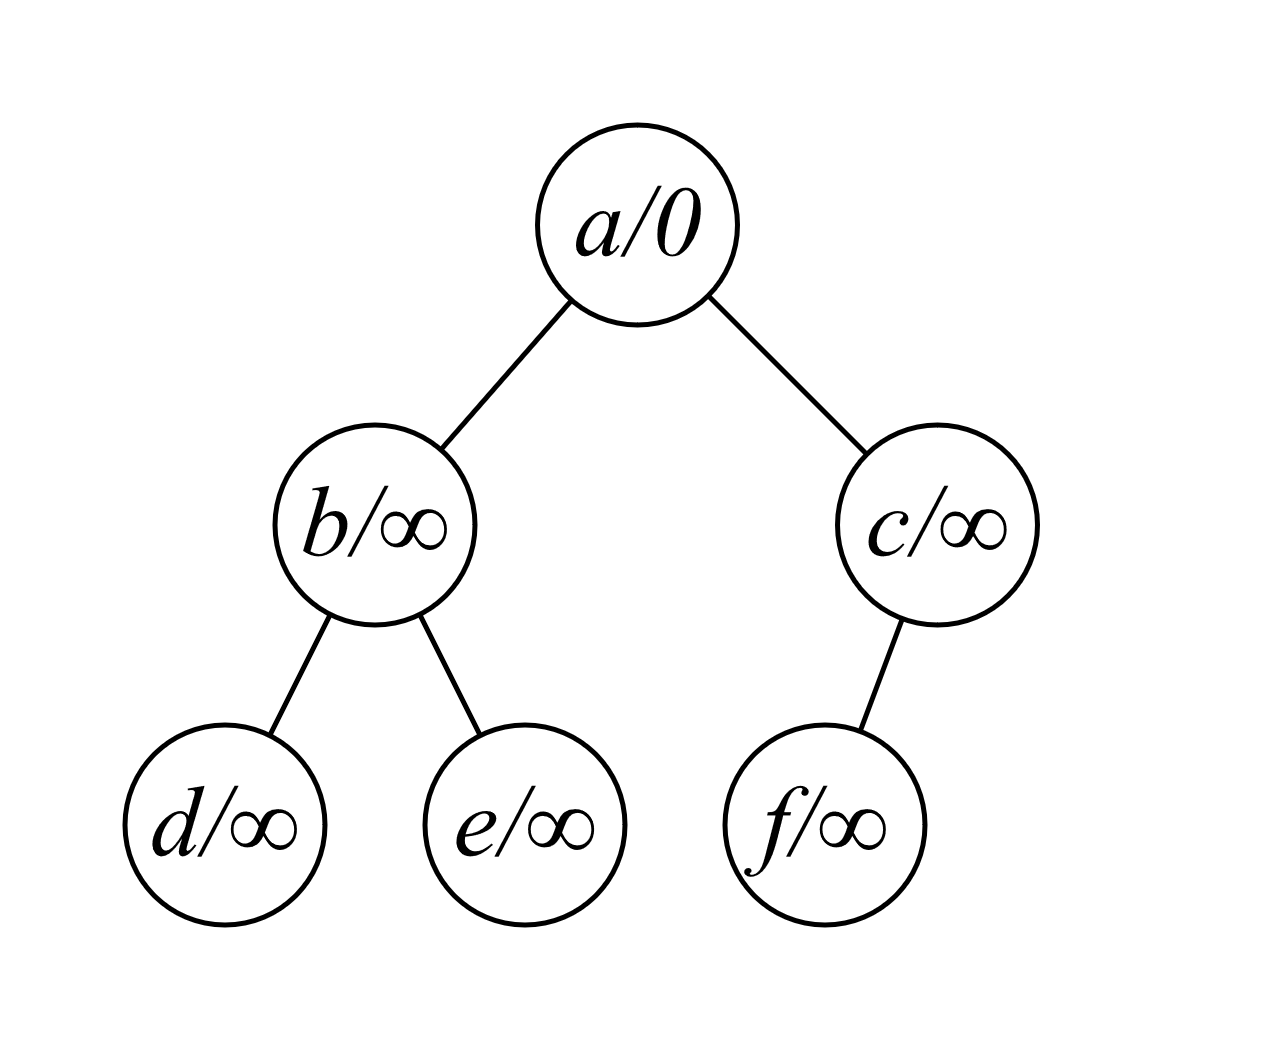
\includegraphics[width=\textwidth]{img/3b_1.png}
            \end{subfigure}
        \end{figure}
        \FloatBarrier
        \begin{figure}[h!]
            \centering
            \begin{subfigure}{0.3\textwidth}
                \centering
                \begin{tikzpicture}[scale=0.15]
                    \tikzstyle{every node}+=[inner sep=0pt]
                    \fill [black] (18.6,-17.6) circle (3);
                    \draw [black] (18.6,-17.6) circle (3);
                    \draw [white] (18.6,-17.6) node {$a$};
                    \draw [black] (31.8,-17.4) circle (3);
                    \draw (31.8,-17.4) node {$b$};
                    \draw [black] (45.4,-17.4) circle (3);
                    \draw (45.4,-17.4) node {$c$};
                    \fill [gray!60] (18.6,-29.1) circle (3);
                    \draw [black] (18.6,-29.1) circle (3);
                    \draw (18.6,-29.1) node {$d$};
                    \draw [black] (31.8,-29.1) circle (3);
                    \draw (31.8,-29.1) node {$e$};
                    \draw [black] (45.4,-29.1) circle (3);
                    \draw (45.4,-29.1) node {$f$};
                    \draw [black, dashed] (21.6,-17.55) -- (28.8,-17.45);
                    \fill [black] (28.8,-17.45) -- (27.99,-16.96) -- (28.01,-17.96);
                    \draw (25.2,-16.98) node [above] {$4$};
                    \draw [black, dashed] (18.6,-20.6) -- (18.6,-26.1);
                    \fill [black] (18.6,-26.1) -- (19.1,-25.3) -- (18.1,-25.3);
                    \draw (18.1,-23.35) node [left] {$2$};
                    \draw [black] (20.85,-27.11) -- (29.55,-19.39);
                    \fill [black] (29.55,-19.39) -- (28.62,-19.55) -- (29.29,-20.29);
                    \draw (24.19,-22.76) node [above] {$1$};
                    \draw [black] (31.8,-20.4) -- (31.8,-26.1);
                    \fill [black] (31.8,-26.1) -- (32.3,-25.3) -- (31.3,-25.3);
                    \draw (31.3,-23.25) node [left] {$2$};
                    \draw [black] (21.6,-29.1) -- (28.8,-29.1);
                    \fill [black] (28.8,-29.1) -- (28,-28.6) -- (28,-29.6);
                    \draw (25.2,-29.6) node [below] {$4$};
                    \draw [black] (30.372,-31.724) arc (-37.69112:-224.43443:9.416);
                    \fill [black] (16.2,-19.37) -- (15.28,-19.6) -- (15.99,-20.3);
                    \draw (15.72,-33.56) node [below] {$1$};
                    \draw [black] (34.8,-17.4) -- (42.4,-17.4);
                    \fill [black] (42.4,-17.4) -- (41.6,-16.9) -- (41.6,-17.9);
                    \draw (38.6,-16.9) node [above] {$3$};
                    \draw [black] (43.789,-19.929) arc (-35.78379:-62.80578:26.108);
                    \fill [black] (43.79,-19.93) -- (42.92,-20.29) -- (43.73,-20.87);
                    \draw (40.65,-24.95) node [below] {$1$};
                    \draw [black] (33.471,-26.61) arc (143.10748:118.30295:28.307);
                    \fill [black] (33.47,-26.61) -- (34.35,-26.27) -- (33.55,-25.67);
                    \draw (36.64,-21.65) node [above] {$1$};
                    \draw [black] (34.8,-29.1) -- (42.4,-29.1);
                    \fill [black] (42.4,-29.1) -- (41.6,-28.6) -- (41.6,-29.6);
                    \draw (38.6,-29.6) node [below] {$3$};
                    \draw [black] (45.4,-20.4) -- (45.4,-26.1);
                    \fill [black] (45.4,-26.1) -- (45.9,-25.3) -- (44.9,-25.3);
                    \draw (45.9,-23.25) node [right] {$1$};
                \end{tikzpicture}
            \end{subfigure}
            \begin{subfigure}{0.3\textwidth}
                \centering
                \begin{tabular}{|c|c|c|c|c|c|}
                    \hline
                    $a$ & $b$ & $c$ & $d$ & $e$ & $f$ \\
                    \hline
                    $0$ & $4$ & $\infty$ & $2$ & $\infty$ & $\infty$ \\
                    \hline
                    $-$ & $a$ & $-$ & $a$ & $-$ & $-$ \\
                    \hline
                \end{tabular}
            \end{subfigure}
            \begin{subfigure}{0.3\textwidth}
                \centering
                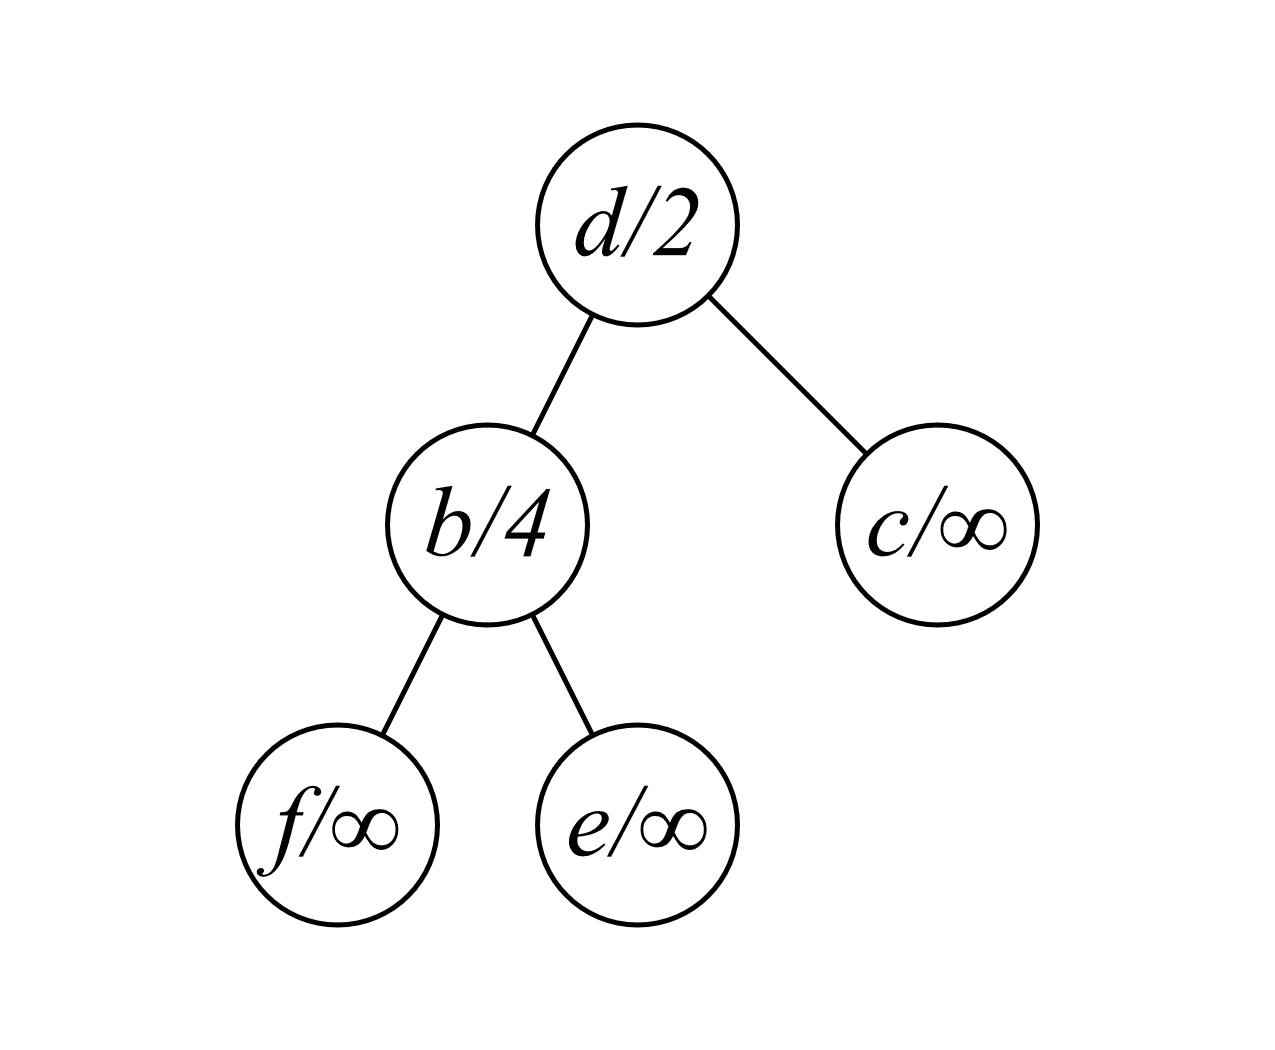
\includegraphics[width=\textwidth]{img/3b_2.png}
            \end{subfigure}
        \end{figure}
        \FloatBarrier
        \begin{figure}[h!]
            \centering
            \begin{subfigure}{0.3\textwidth}
                \centering
                \begin{tikzpicture}[scale=0.15]
                    \tikzstyle{every node}+=[inner sep=0pt]
                    \fill [black] (18.6,-17.6) circle (3);
                    \draw [black] (18.6,-17.6) circle (3);
                    \draw [white] (18.6,-17.6) node {$a$};
                    \fill [gray!60] (31.8,-17.4) circle (3);
                    \draw [black] (31.8,-17.4) circle (3);
                    \draw (31.8,-17.4) node {$b$};
                    \draw [black] (45.4,-17.4) circle (3);
                    \draw (45.4,-17.4) node {$c$};
                    \fill [black] (18.6,-29.1) circle (3);
                    \draw [black] (18.6,-29.1) circle (3);
                    \draw [white] (18.6,-29.1) node {$d$};
                    \draw [black] (31.8,-29.1) circle (3);
                    \draw (31.8,-29.1) node {$e$};
                    \draw [black] (45.4,-29.1) circle (3);
                    \draw (45.4,-29.1) node {$f$};
                    \draw [black] (21.6,-17.55) -- (28.8,-17.45);
                    \fill [black] (28.8,-17.45) -- (27.99,-16.96) -- (28.01,-17.96);
                    \draw (25.2,-16.98) node [above] {$4$};
                    \draw [black, dashed] (18.6,-20.6) -- (18.6,-26.1);
                    \fill [black] (18.6,-26.1) -- (19.1,-25.3) -- (18.1,-25.3);
                    \draw (18.1,-23.35) node [left] {$2$};
                    \draw [black, dashed] (20.85,-27.11) -- (29.55,-19.39);
                    \fill [black] (29.55,-19.39) -- (28.62,-19.55) -- (29.29,-20.29);
                    \draw (24.19,-22.76) node [above] {$1$};
                    \draw [black] (31.8,-20.4) -- (31.8,-26.1);
                    \fill [black] (31.8,-26.1) -- (32.3,-25.3) -- (31.3,-25.3);
                    \draw (31.3,-23.25) node [left] {$2$};
                    \draw [black, dashed] (21.6,-29.1) -- (28.8,-29.1);
                    \fill [black] (28.8,-29.1) -- (28,-28.6) -- (28,-29.6);
                    \draw (25.2,-29.6) node [below] {$4$};
                    \draw [black] (30.372,-31.724) arc (-37.69112:-224.43443:9.416);
                    \fill [black] (16.2,-19.37) -- (15.28,-19.6) -- (15.99,-20.3);
                    \draw (15.72,-33.56) node [below] {$1$};
                    \draw [black] (34.8,-17.4) -- (42.4,-17.4);
                    \fill [black] (42.4,-17.4) -- (41.6,-16.9) -- (41.6,-17.9);
                    \draw (38.6,-16.9) node [above] {$3$};
                    \draw [black] (43.789,-19.929) arc (-35.78379:-62.80578:26.108);
                    \fill [black] (43.79,-19.93) -- (42.92,-20.29) -- (43.73,-20.87);
                    \draw (40.65,-24.95) node [below] {$1$};
                    \draw [black] (33.471,-26.61) arc (143.10748:118.30295:28.307);
                    \fill [black] (33.47,-26.61) -- (34.35,-26.27) -- (33.55,-25.67);
                    \draw (36.64,-21.65) node [above] {$1$};
                    \draw [black] (34.8,-29.1) -- (42.4,-29.1);
                    \fill [black] (42.4,-29.1) -- (41.6,-28.6) -- (41.6,-29.6);
                    \draw (38.6,-29.6) node [below] {$3$};
                    \draw [black] (45.4,-20.4) -- (45.4,-26.1);
                    \fill [black] (45.4,-26.1) -- (45.9,-25.3) -- (44.9,-25.3);
                    \draw (45.9,-23.25) node [right] {$1$};
                \end{tikzpicture}
            \end{subfigure}
            \begin{subfigure}{0.3\textwidth}
                \centering
                \begin{tabular}{|c|c|c|c|c|c|}
                    \hline
                    $a$ & $b$ & $c$ & $d$ & $e$ & $f$ \\
                    \hline
                    $0$ & $3$ & $\infty$ & $2$ & $6$ & $\infty$ \\
                    \hline
                    $-$ & $d$ & $-$ & $a$ & $d$ & $-$ \\
                    \hline
                \end{tabular}
            \end{subfigure}
            \begin{subfigure}{0.3\textwidth}
                \centering
                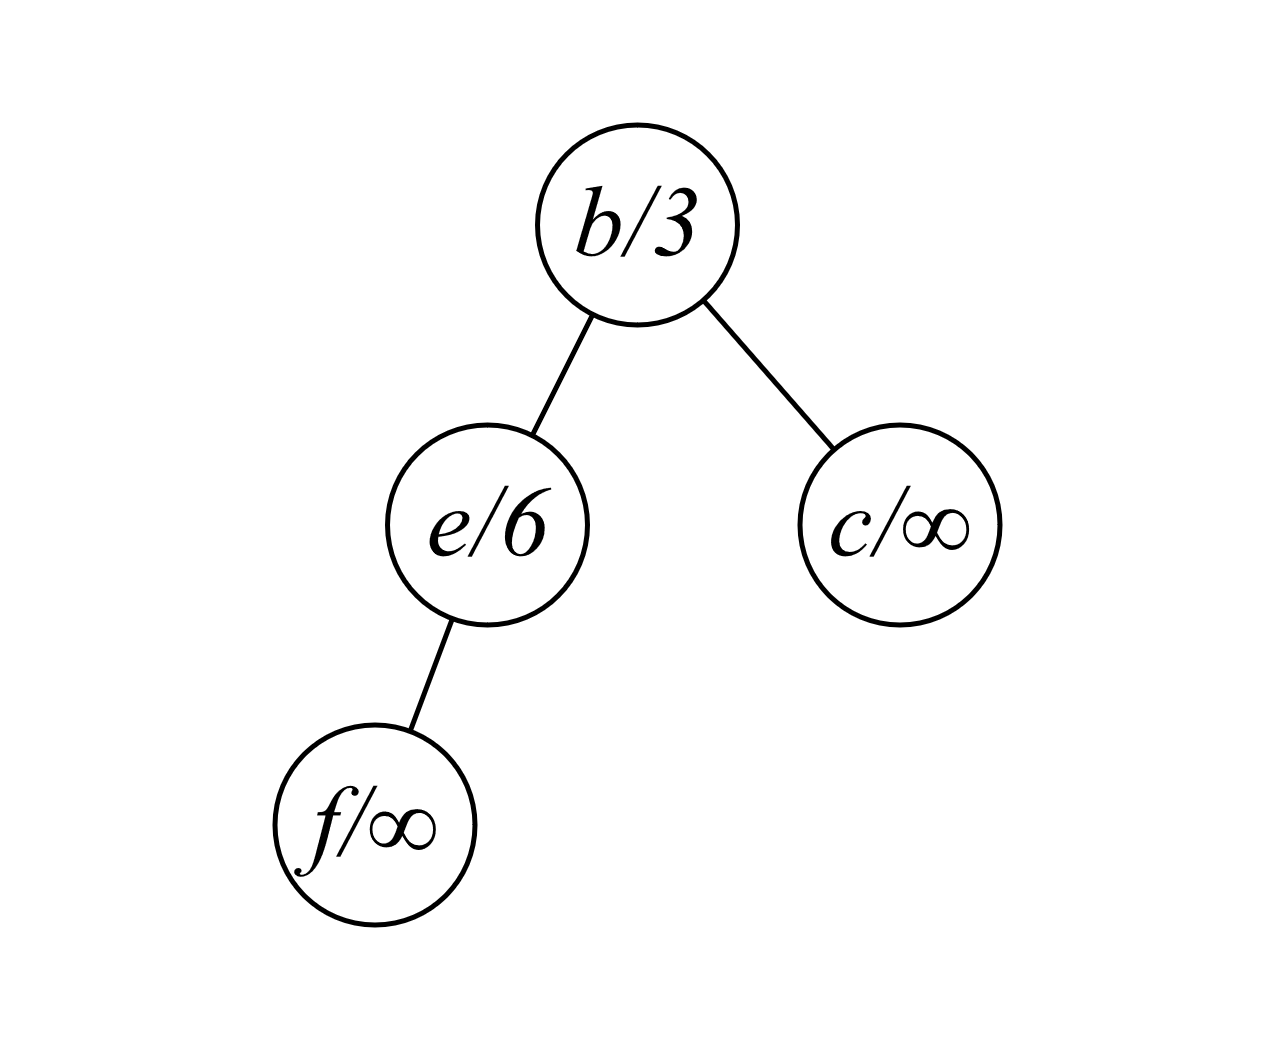
\includegraphics[width=\textwidth]{img/3b_3.png}
            \end{subfigure}
        \end{figure}
        \FloatBarrier
        \begin{figure}[h!]
            \centering
            \begin{subfigure}{0.3\textwidth}
                \centering
                \begin{tikzpicture}[scale=0.15]
                    \tikzstyle{every node}+=[inner sep=0pt]
                    \fill [black] (18.6,-17.6) circle (3);
                    \draw [black] (18.6,-17.6) circle (3);
                    \draw [white] (18.6,-17.6) node {$a$};
                    \fill [black] (31.8,-17.4) circle (3);
                    \draw [black] (31.8,-17.4) circle (3);
                    \draw [white] (31.8,-17.4) node {$b$};
                    \draw [black] (45.4,-17.4) circle (3);
                    \draw (45.4,-17.4) node {$c$};
                    \fill [black] (18.6,-29.1) circle (3);
                    \draw [black] (18.6,-29.1) circle (3);
                    \draw [white] (18.6,-29.1) node {$d$};
                    \fill [gray!60] (31.8,-29.1) circle (3);
                    \draw [black] (31.8,-29.1) circle (3);
                    \draw (31.8,-29.1) node {$e$};
                    \draw [black] (45.4,-29.1) circle (3);
                    \draw (45.4,-29.1) node {$f$};
                    \draw [black] (21.6,-17.55) -- (28.8,-17.45);
                    \fill [black] (28.8,-17.45) -- (27.99,-16.96) -- (28.01,-17.96);
                    \draw (25.2,-16.98) node [above] {$4$};
                    \draw [black, dashed] (18.6,-20.6) -- (18.6,-26.1);
                    \fill [black] (18.6,-26.1) -- (19.1,-25.3) -- (18.1,-25.3);
                    \draw (18.1,-23.35) node [left] {$2$};
                    \draw [black, dashed] (20.85,-27.11) -- (29.55,-19.39);
                    \fill [black] (29.55,-19.39) -- (28.62,-19.55) -- (29.29,-20.29);
                    \draw (24.19,-22.76) node [above] {$1$};
                    \draw [black, dashed] (31.8,-20.4) -- (31.8,-26.1);
                    \fill [black] (31.8,-26.1) -- (32.3,-25.3) -- (31.3,-25.3);
                    \draw (31.3,-23.25) node [left] {$2$};
                    \draw [black] (21.6,-29.1) -- (28.8,-29.1);
                    \fill [black] (28.8,-29.1) -- (28,-28.6) -- (28,-29.6);
                    \draw (25.2,-29.6) node [below] {$4$};
                    \draw [black] (30.372,-31.724) arc (-37.69112:-224.43443:9.416);
                    \fill [black] (16.2,-19.37) -- (15.28,-19.6) -- (15.99,-20.3);
                    \draw (15.72,-33.56) node [below] {$1$};
                    \draw [black, dashed] (34.8,-17.4) -- (42.4,-17.4);
                    \fill [black] (42.4,-17.4) -- (41.6,-16.9) -- (41.6,-17.9);
                    \draw (38.6,-16.9) node [above] {$3$};
                    \draw [black] (43.789,-19.929) arc (-35.78379:-62.80578:26.108);
                    \fill [black] (43.79,-19.93) -- (42.92,-20.29) -- (43.73,-20.87);
                    \draw (40.65,-24.95) node [below] {$1$};
                    \draw [black] (33.471,-26.61) arc (143.10748:118.30295:28.307);
                    \fill [black] (33.47,-26.61) -- (34.35,-26.27) -- (33.55,-25.67);
                    \draw (36.64,-21.65) node [above] {$1$};
                    \draw [black] (34.8,-29.1) -- (42.4,-29.1);
                    \fill [black] (42.4,-29.1) -- (41.6,-28.6) -- (41.6,-29.6);
                    \draw (38.6,-29.6) node [below] {$3$};
                    \draw [black] (45.4,-20.4) -- (45.4,-26.1);
                    \fill [black] (45.4,-26.1) -- (45.9,-25.3) -- (44.9,-25.3);
                    \draw (45.9,-23.25) node [right] {$1$};
                \end{tikzpicture}
            \end{subfigure}
            \begin{subfigure}{0.3\textwidth}
                \centering
                \begin{tabular}{|c|c|c|c|c|c|}
                    \hline
                    $a$ & $b$ & $c$ & $d$ & $e$ & $f$ \\
                    \hline
                    $0$ & $3$ & $6$ & $2$ & $5$ & $\infty$ \\
                    \hline
                    $-$ & $d$ & $b$ & $a$ & $b$ & $-$ \\
                    \hline
                \end{tabular}
            \end{subfigure}
            \begin{subfigure}{0.3\textwidth}
                \centering
                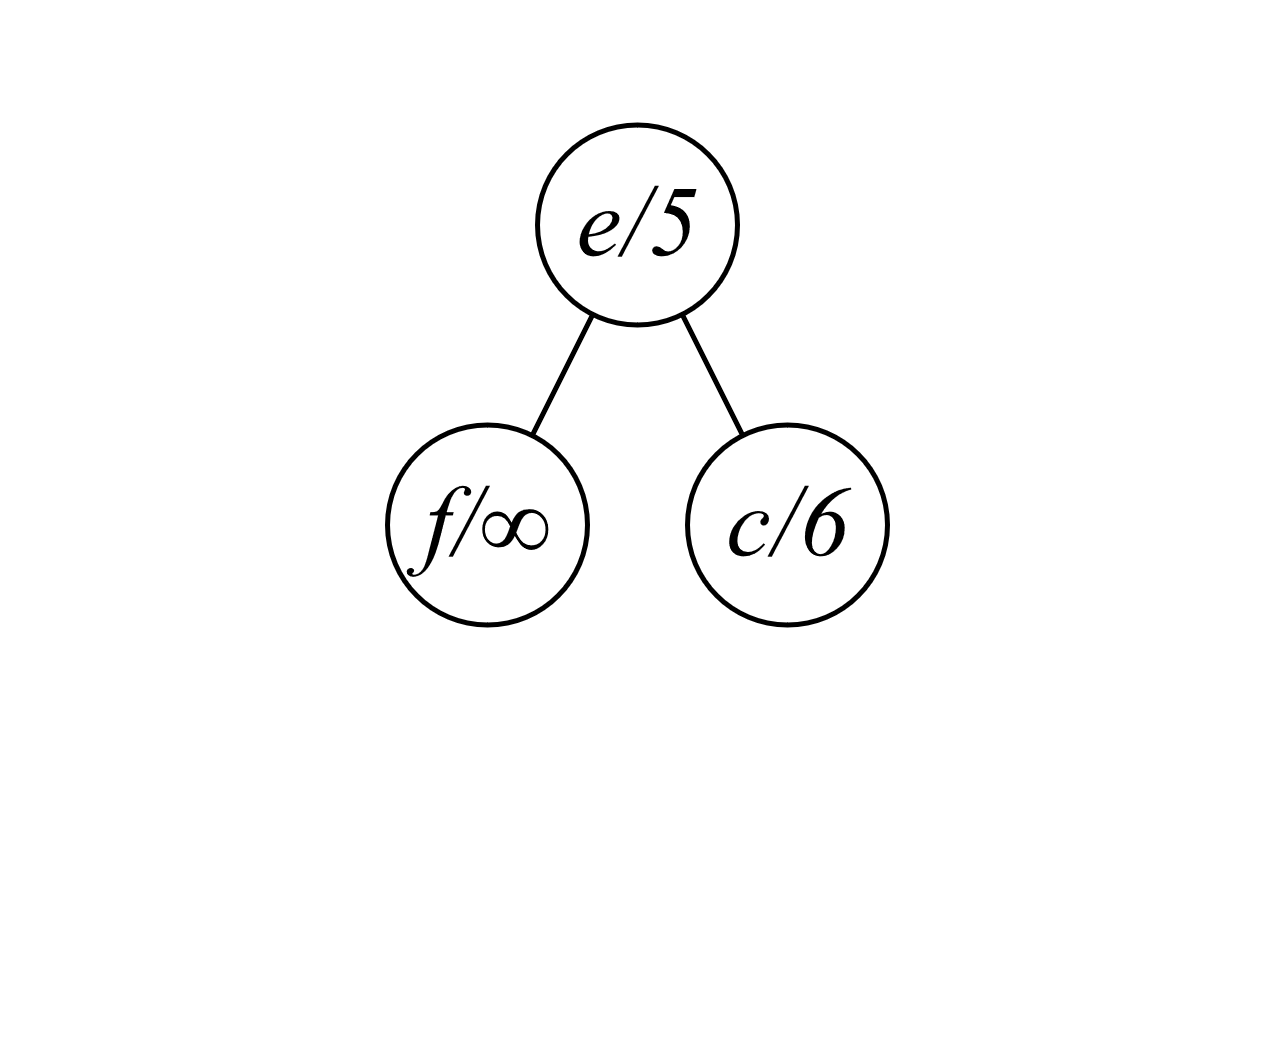
\includegraphics[width=\textwidth]{img/3b_4.png}
            \end{subfigure}
        \end{figure}
        \FloatBarrier
        \begin{figure}[h!]
            \centering
            \begin{subfigure}{0.3\textwidth}
                \centering
                \begin{tikzpicture}[scale=0.15]
                    \tikzstyle{every node}+=[inner sep=0pt]
                    \fill [black] (18.6,-17.6) circle (3);
                    \draw [black] (18.6,-17.6) circle (3);
                    \draw [white] (18.6,-17.6) node {$a$};
                    \fill [black] (31.8,-17.4) circle (3);
                    \draw [black] (31.8,-17.4) circle (3);
                    \draw [white] (31.8,-17.4) node {$b$};
                    \fill [gray!60] (45.4,-17.4) circle (3);
                    \draw [black] (45.4,-17.4) circle (3);
                    \draw (45.4,-17.4) node {$c$};
                    \fill [black] (18.6,-29.1) circle (3);
                    \draw [black] (18.6,-29.1) circle (3);
                    \draw [white] (18.6,-29.1) node {$d$};
                    \fill [black] (31.8,-29.1) circle (3);
                    \draw [black] (31.8,-29.1) circle (3);
                    \draw [white] (31.8,-29.1) node {$e$};
                    \draw [black] (45.4,-29.1) circle (3);
                    \draw (45.4,-29.1) node {$f$};
                    \draw [black] (21.6,-17.55) -- (28.8,-17.45);
                    \fill [black] (28.8,-17.45) -- (27.99,-16.96) -- (28.01,-17.96);
                    \draw (25.2,-16.98) node [above] {$4$};
                    \draw [black, dashed] (18.6,-20.6) -- (18.6,-26.1);
                    \fill [black] (18.6,-26.1) -- (19.1,-25.3) -- (18.1,-25.3);
                    \draw (18.1,-23.35) node [left] {$2$};
                    \draw [black, dashed] (20.85,-27.11) -- (29.55,-19.39);
                    \fill [black] (29.55,-19.39) -- (28.62,-19.55) -- (29.29,-20.29);
                    \draw (24.19,-22.76) node [above] {$1$};
                    \draw [black, dashed] (31.8,-20.4) -- (31.8,-26.1);
                    \fill [black] (31.8,-26.1) -- (32.3,-25.3) -- (31.3,-25.3);
                    \draw (31.3,-23.25) node [left] {$2$};
                    \draw [black] (21.6,-29.1) -- (28.8,-29.1);
                    \fill [black] (28.8,-29.1) -- (28,-28.6) -- (28,-29.6);
                    \draw (25.2,-29.6) node [below] {$4$};
                    \draw [black] (30.372,-31.724) arc (-37.69112:-224.43443:9.416);
                    \fill [black] (16.2,-19.37) -- (15.28,-19.6) -- (15.99,-20.3);
                    \draw (15.72,-33.56) node [below] {$1$};
                    \draw [black, dashed] (34.8,-17.4) -- (42.4,-17.4);
                    \fill [black] (42.4,-17.4) -- (41.6,-16.9) -- (41.6,-17.9);
                    \draw (38.6,-16.9) node [above] {$3$};
                    \draw [black] (43.789,-19.929) arc (-35.78379:-62.80578:26.108);
                    \fill [black] (43.79,-19.93) -- (42.92,-20.29) -- (43.73,-20.87);
                    \draw (40.65,-24.95) node [below] {$1$};
                    \draw [black] (33.471,-26.61) arc (143.10748:118.30295:28.307);
                    \fill [black] (33.47,-26.61) -- (34.35,-26.27) -- (33.55,-25.67);
                    \draw (36.64,-21.65) node [above] {$1$};
                    \draw [black, dashed] (34.8,-29.1) -- (42.4,-29.1);
                    \fill [black] (42.4,-29.1) -- (41.6,-28.6) -- (41.6,-29.6);
                    \draw (38.6,-29.6) node [below] {$3$};
                    \draw [black] (45.4,-20.4) -- (45.4,-26.1);
                    \fill [black] (45.4,-26.1) -- (45.9,-25.3) -- (44.9,-25.3);
                    \draw (45.9,-23.25) node [right] {$1$};
                \end{tikzpicture}
            \end{subfigure}
            \begin{subfigure}{0.3\textwidth}
                \centering
                \begin{tabular}{|c|c|c|c|c|c|}
                    \hline
                    $a$ & $b$ & $c$ & $d$ & $e$ & $f$ \\
                    \hline
                    $0$ & $3$ & $6$ & $2$ & $5$ & $8$ \\
                    \hline
                    $-$ & $d$ & $b$ & $a$ & $b$ & $e$ \\
                    \hline
                \end{tabular}
            \end{subfigure}
            \begin{subfigure}{0.3\textwidth}
                \centering
                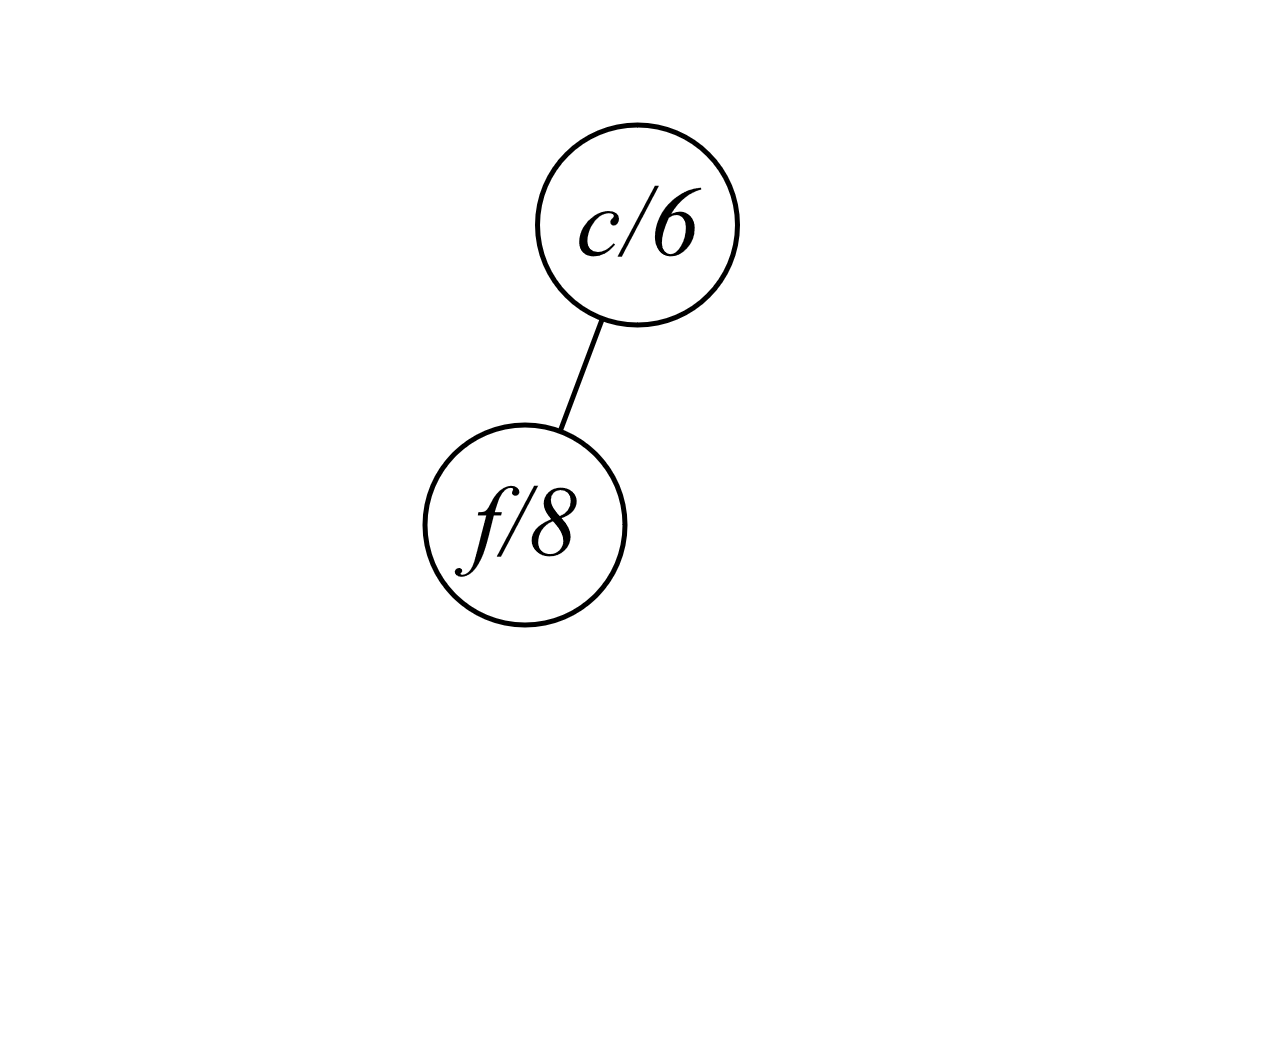
\includegraphics[width=\textwidth]{img/3b_5.png}
            \end{subfigure}
        \end{figure}
        \begin{figure}[h!]
            \centering
            \begin{subfigure}{0.3\textwidth}
                \centering
                \begin{tikzpicture}[scale=0.15]
                    \tikzstyle{every node}+=[inner sep=0pt]
                    \fill [black] (18.6,-17.6) circle (3);
                    \draw [black] (18.6,-17.6) circle (3);
                    \draw [white] (18.6,-17.6) node {$a$};
                    \fill [black] (31.8,-17.4) circle (3);
                    \draw [black] (31.8,-17.4) circle (3);
                    \draw [white] (31.8,-17.4) node {$b$};
                    \fill [black] (45.4,-17.4) circle (3);
                    \draw [black] (45.4,-17.4) circle (3);
                    \draw [white] (45.4,-17.4) node {$c$};
                    \fill [black] (18.6,-29.1) circle (3);
                    \draw [black] (18.6,-29.1) circle (3);
                    \draw [white] (18.6,-29.1) node {$d$};
                    \fill [black] (31.8,-29.1) circle (3);
                    \draw [black] (31.8,-29.1) circle (3);
                    \draw [white] (31.8,-29.1) node {$e$};
                    \fill [gray!60] (45.4,-29.1) circle (3);
                    \draw [black] (45.4,-29.1) circle (3);
                    \draw (45.4,-29.1) node {$f$};
                    \draw [black] (21.6,-17.55) -- (28.8,-17.45);
                    \fill [black] (28.8,-17.45) -- (27.99,-16.96) -- (28.01,-17.96);
                    \draw (25.2,-16.98) node [above] {$4$};
                    \draw [black, dashed] (18.6,-20.6) -- (18.6,-26.1);
                    \fill [black] (18.6,-26.1) -- (19.1,-25.3) -- (18.1,-25.3);
                    \draw (18.1,-23.35) node [left] {$2$};
                    \draw [black, dashed] (20.85,-27.11) -- (29.55,-19.39);
                    \fill [black] (29.55,-19.39) -- (28.62,-19.55) -- (29.29,-20.29);
                    \draw (24.19,-22.76) node [above] {$1$};
                    \draw [black, dashed] (31.8,-20.4) -- (31.8,-26.1);
                    \fill [black] (31.8,-26.1) -- (32.3,-25.3) -- (31.3,-25.3);
                    \draw (31.3,-23.25) node [left] {$2$};
                    \draw [black] (21.6,-29.1) -- (28.8,-29.1);
                    \fill [black] (28.8,-29.1) -- (28,-28.6) -- (28,-29.6);
                    \draw (25.2,-29.6) node [below] {$4$};
                    \draw [black] (30.372,-31.724) arc (-37.69112:-224.43443:9.416);
                    \fill [black] (16.2,-19.37) -- (15.28,-19.6) -- (15.99,-20.3);
                    \draw (15.72,-33.56) node [below] {$1$};
                    \draw [black, dashed] (34.8,-17.4) -- (42.4,-17.4);
                    \fill [black] (42.4,-17.4) -- (41.6,-16.9) -- (41.6,-17.9);
                    \draw (38.6,-16.9) node [above] {$3$};
                    \draw [black] (43.789,-19.929) arc (-35.78379:-62.80578:26.108);
                    \fill [black] (43.79,-19.93) -- (42.92,-20.29) -- (43.73,-20.87);
                    \draw (40.65,-24.95) node [below] {$1$};
                    \draw [black] (33.471,-26.61) arc (143.10748:118.30295:28.307);
                    \fill [black] (33.47,-26.61) -- (34.35,-26.27) -- (33.55,-25.67);
                    \draw (36.64,-21.65) node [above] {$1$};
                    \draw [black] (34.8,-29.1) -- (42.4,-29.1);
                    \fill [black] (42.4,-29.1) -- (41.6,-28.6) -- (41.6,-29.6);
                    \draw (38.6,-29.6) node [below] {$3$};
                    \draw [black, dashed] (45.4,-20.4) -- (45.4,-26.1);
                    \fill [black] (45.4,-26.1) -- (45.9,-25.3) -- (44.9,-25.3);
                    \draw (45.9,-23.25) node [right] {$1$};
                \end{tikzpicture}
            \end{subfigure}
            \begin{subfigure}{0.3\textwidth}
                \centering
                \begin{tabular}{|c|c|c|c|c|c|}
                    \hline
                    $a$ & $b$ & $c$ & $d$ & $e$ & $f$ \\
                    \hline
                    $0$ & $3$ & $6$ & $2$ & $5$ & $7$ \\
                    \hline
                    $-$ & $d$ & $b$ & $a$ & $b$ & $c$ \\
                    \hline
                \end{tabular}
            \end{subfigure}
            \begin{subfigure}{0.3\textwidth}
                \centering
                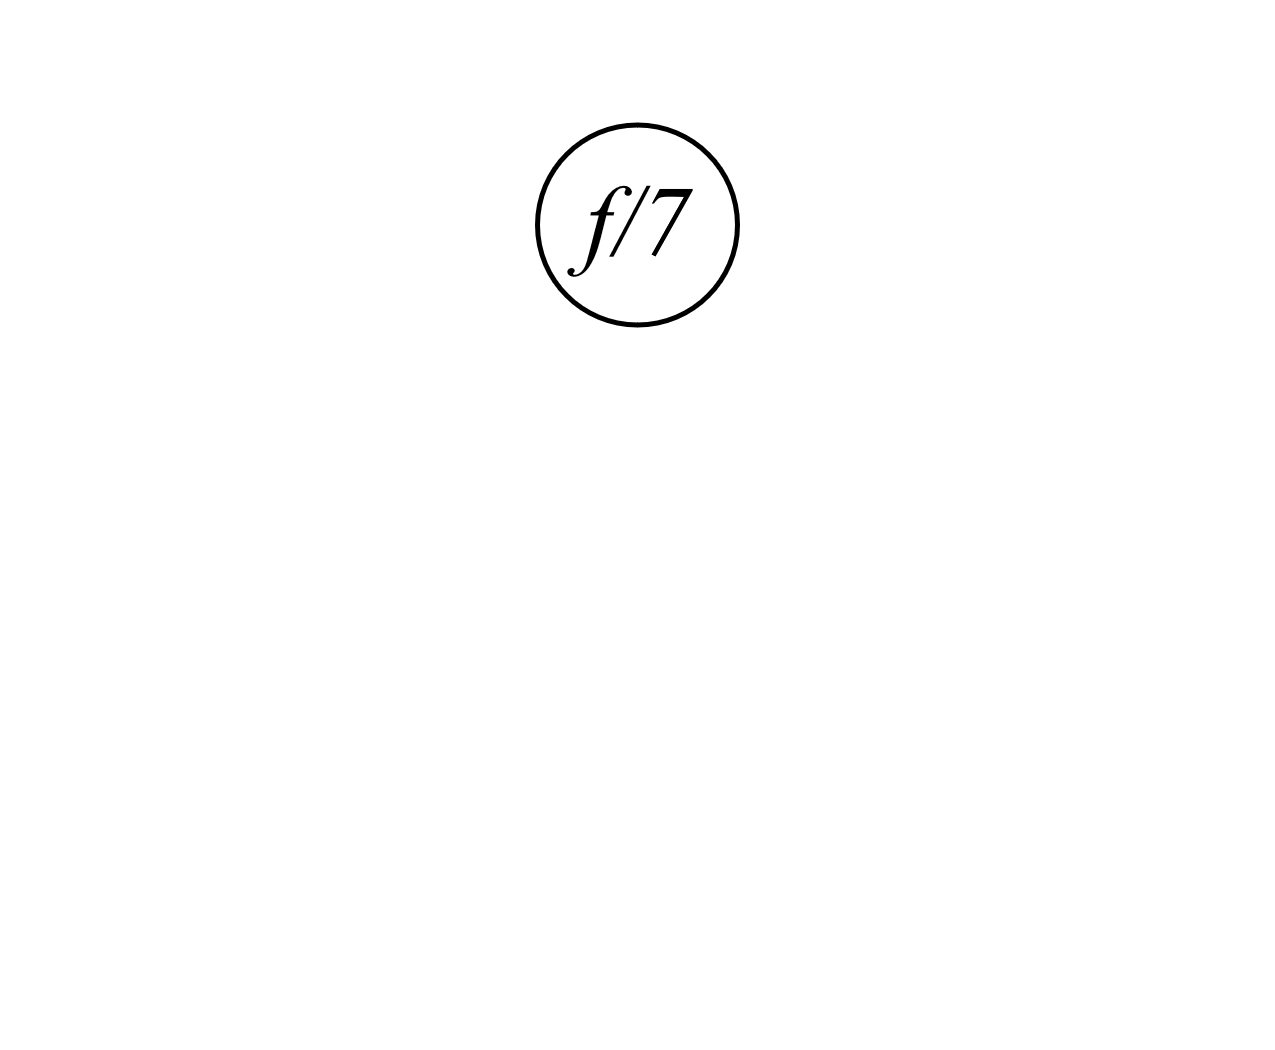
\includegraphics[width=\textwidth]{img/3b_6.png}
            \end{subfigure}
        \end{figure}
        \FloatBarrier
        
        \item \ \\
        \begin{figure}[h!]
            \centering
            \begin{subfigure}{0.45\textwidth}
                \centering
                \begin{tikzpicture}[scale=0.13]
                    \tikzstyle{every node}+=[inner sep=0pt]
                    \fill [gray!60] (16.1,-16.8) circle (3);
                    \draw [black] (16.1,-16.8) circle (3);
                    \draw (16.1,-16.8) node {$1$};
                    \draw [black] (32.1,-16.8) circle (3);
                    \draw (32.1,-16.8) node {$2$};
                    \draw [black] (16.1,-31.8) circle (3);
                    \draw (16.1,-31.8) node {$4$};
                    \draw [black] (32.1,-31.8) circle (3);
                    \draw (32.1,-31.8) node {$5$};
                    \draw [black] (47.8,-31.8) circle (3);
                    \draw (47.8,-31.8) node {$6$};
                    \draw [black] (47.8,-16.8) circle (3);
                    \draw (47.8,-16.8) node {$3$};
                    \draw [black] (16.1,-47.2) circle (3);
                    \draw (16.1,-47.2) node {$7$};
                    \draw [black] (32.1,-47.2) circle (3);
                    \draw (32.1,-47.2) node {$8$};
                    \draw [black] (47.8,-47.2) circle (3);
                    \draw (47.8,-47.2) node {$9$};
                    \draw [black] (34.27,-29.73) -- (45.63,-18.87);
                    \draw (38.93,-23.82) node [above] {$1$};
                    \draw [black] (44.8,-31.8) -- (35.1,-31.8);
                    \draw (39.95,-31.3) node [above] {$2$};
                    \draw [black] (47.8,-28.8) -- (47.8,-19.8);
                    \draw (47.3,-24.3) node [left] {$3$};
                    \draw [black] (19.1,-47.2) -- (29.1,-47.2);
                    \draw (24.1,-46.7) node [above] {$4$};
                    \draw [black] (18.29,-29.75) -- (29.91,-18.85);
                    \draw (23.08,-23.82) node [above] {$5$};
                    \draw [black] (19.1,-31.8) -- (29.1,-31.8);
                    \draw (24.1,-31.3) node [above] {$6$};
                    \draw [black] (16.1,-34.8) -- (16.1,-44.2);
                    \draw (15.6,-39.5) node [left] {$7$};
                    \draw [black] (32.1,-34.8) -- (32.1,-44.2);
                    \draw (31.6,-39.5) node [left] {$8$};
                    \draw [black] (35.1,-16.8) -- (44.8,-16.8);
                    \draw (39.95,-16.3) node [above] {$9$};
                    \draw [black] (19.1,-16.8) -- (29.1,-16.8);
                    \draw (24.1,-16.3) node [above] {$10$};
                    \draw [black] (16.1,-19.8) -- (16.1,-28.8);
                    \draw (15.6,-24.3) node [left] {$11$};
                    \draw [black] (47.8,-34.8) -- (47.8,-44.2);
                    \draw (47.3,-39.5) node [left] {$13$};
                    \draw [black] (35.1,-47.2) -- (44.8,-47.2);
                    \draw (39.95,-46.7) node [above] {$14$};
                    \draw [black] (34.24,-45.1) -- (45.66,-33.9);
                    \draw (38.43,-39.02) node [above] {$12$};
                    \draw [black] (18.26,-45.12) -- (29.94,-33.88);
                    \draw (22.58,-39.02) node [above] {$15$};
                    \draw [black] (32.1,-28.8) -- (32.1,-19.8);
                    \draw (31.6,-24.3) node [left] {$16$};
                \end{tikzpicture}
            \end{subfigure}
            \begin{subfigure}{0.45\textwidth}
                \begin{tabular}{|c|c|c|c|c|c|c|c|c|}
                    \hline
                    $1$ & $2$ & $3$ & $4$ & $5$ & $6$ & $7$ & $8$ & $9$ \\
                    \hline
                    $0$ & $\infty$ & $\infty$ & $\infty$ & $\infty$ & $\infty$ & $\infty$ & $\infty$ & $\infty$ \\
                    \hline
                    $-$ & $-$ & $-$ & $-$ & $-$ & $-$ & $-$ & $-$ & $-$ \\
                    \hline
                \end{tabular}
            \end{subfigure}
        \end{figure}
        \begin{figure}[h!]
            \centering
            \begin{subfigure}{0.45\textwidth}
                \centering
                \begin{tikzpicture}[scale=0.13]
                    \tikzstyle{every node}+=[inner sep=0pt]
                    \fill [black] (16.1,-16.8) circle (3);
                    \draw [black] (16.1,-16.8) circle (3);
                    \draw [white] (16.1,-16.8) node {$1$};
                    \fill [gray!60] (32.1,-16.8) circle (3);
                    \draw [black] (32.1,-16.8) circle (3);
                    \draw (32.1,-16.8) node {$2$};
                    \draw [black] (16.1,-31.8) circle (3);
                    \draw (16.1,-31.8) node {$4$};
                    \draw [black] (32.1,-31.8) circle (3);
                    \draw (32.1,-31.8) node {$5$};
                    \draw [black] (47.8,-31.8) circle (3);
                    \draw (47.8,-31.8) node {$6$};
                    \draw [black] (47.8,-16.8) circle (3);
                    \draw (47.8,-16.8) node {$3$};
                    \draw [black] (16.1,-47.2) circle (3);
                    \draw (16.1,-47.2) node {$7$};
                    \draw [black] (32.1,-47.2) circle (3);
                    \draw (32.1,-47.2) node {$8$};
                    \draw [black] (47.8,-47.2) circle (3);
                    \draw (47.8,-47.2) node {$9$};
                    \draw [black] (34.27,-29.73) -- (45.63,-18.87);
                    \draw (38.93,-23.82) node [above] {$1$};
                    \draw [black] (44.8,-31.8) -- (35.1,-31.8);
                    \draw (39.95,-31.3) node [above] {$2$};
                    \draw [black] (47.8,-28.8) -- (47.8,-19.8);
                    \draw (47.3,-24.3) node [left] {$3$};
                    \draw [black] (19.1,-47.2) -- (29.1,-47.2);
                    \draw (24.1,-46.7) node [above] {$4$};
                    \draw [black] (18.29,-29.75) -- (29.91,-18.85);
                    \draw (23.08,-23.82) node [above] {$5$};
                    \draw [black] (19.1,-31.8) -- (29.1,-31.8);
                    \draw (24.1,-31.3) node [above] {$6$};
                    \draw [black] (16.1,-34.8) -- (16.1,-44.2);
                    \draw (15.6,-39.5) node [left] {$7$};
                    \draw [black] (32.1,-34.8) -- (32.1,-44.2);
                    \draw (31.6,-39.5) node [left] {$8$};
                    \draw [black] (35.1,-16.8) -- (44.8,-16.8);
                    \draw (39.95,-16.3) node [above] {$9$};
                    \draw [black, dashed] (19.1,-16.8) -- (29.1,-16.8);
                    \draw (24.1,-16.3) node [above] {$10$};
                    \draw [black, dashed] (16.1,-19.8) -- (16.1,-28.8);
                    \draw (15.6,-24.3) node [left] {$11$};
                    \draw [black] (47.8,-34.8) -- (47.8,-44.2);
                    \draw (47.3,-39.5) node [left] {$13$};
                    \draw [black] (35.1,-47.2) -- (44.8,-47.2);
                    \draw (39.95,-46.7) node [above] {$14$};
                    \draw [black] (34.24,-45.1) -- (45.66,-33.9);
                    \draw (38.43,-39.02) node [above] {$12$};
                    \draw [black] (18.26,-45.12) -- (29.94,-33.88);
                    \draw (22.58,-39.02) node [above] {$15$};
                    \draw [black] (32.1,-28.8) -- (32.1,-19.8);
                    \draw (31.6,-24.3) node [left] {$16$};
                \end{tikzpicture}
            \end{subfigure}
            \begin{subfigure}{0.45\textwidth}
                \begin{tabular}{|c|c|c|c|c|c|c|c|c|}
                    \hline
                    $1$ & $2$ & $3$ & $4$ & $5$ & $6$ & $7$ & $8$ & $9$ \\
                    \hline
                    $0$ & $10$ & $\infty$ & $11$ & $\infty$ & $\infty$ & $\infty$ & $\infty$ & $\infty$ \\
                    \hline
                    $-$ & $1$ & $-$ & $1$ & $-$ & $-$ & $-$ & $-$ & $-$ \\
                    \hline
                \end{tabular}
            \end{subfigure}
        \end{figure}
        \begin{figure}[h!]
            \centering
            \begin{subfigure}{0.45\textwidth}
                \centering
                \begin{tikzpicture}[scale=0.13]
                    \tikzstyle{every node}+=[inner sep=0pt]
                    \fill [black] (16.1,-16.8) circle (3);
                    \draw [black] (16.1,-16.8) circle (3);
                    \draw [white] (16.1,-16.8) node {$1$};
                    \fill [black] (32.1,-16.8) circle (3);
                    \draw [black] (32.1,-16.8) circle (3);
                    \draw [white] (32.1,-16.8) node {$2$};
                    \fill [gray!60] (16.1,-31.8) circle (3);
                    \draw [black] (16.1,-31.8) circle (3);
                    \draw (16.1,-31.8) node {$4$};
                    \draw [black] (32.1,-31.8) circle (3);
                    \draw (32.1,-31.8) node {$5$};
                    \draw [black] (47.8,-31.8) circle (3);
                    \draw (47.8,-31.8) node {$6$};
                    \draw [black] (47.8,-16.8) circle (3);
                    \draw (47.8,-16.8) node {$3$};
                    \draw [black] (16.1,-47.2) circle (3);
                    \draw (16.1,-47.2) node {$7$};
                    \draw [black] (32.1,-47.2) circle (3);
                    \draw (32.1,-47.2) node {$8$};
                    \draw [black] (47.8,-47.2) circle (3);
                    \draw (47.8,-47.2) node {$9$};
                    \draw [black] (34.27,-29.73) -- (45.63,-18.87);
                    \draw (38.93,-23.82) node [above] {$1$};
                    \draw [black] (44.8,-31.8) -- (35.1,-31.8);
                    \draw (39.95,-31.3) node [above] {$2$};
                    \draw [black] (47.8,-28.8) -- (47.8,-19.8);
                    \draw (47.3,-24.3) node [left] {$3$};
                    \draw [black] (19.1,-47.2) -- (29.1,-47.2);
                    \draw (24.1,-46.7) node [above] {$4$};
                    \draw [black] (18.29,-29.75) -- (29.91,-18.85);
                    \draw (23.08,-23.82) node [above] {$5$};
                    \draw [black] (19.1,-31.8) -- (29.1,-31.8);
                    \draw (24.1,-31.3) node [above] {$6$};
                    \draw [black] (16.1,-34.8) -- (16.1,-44.2);
                    \draw (15.6,-39.5) node [left] {$7$};
                    \draw [black] (32.1,-34.8) -- (32.1,-44.2);
                    \draw (31.6,-39.5) node [left] {$8$};
                    \draw [black, dashed] (35.1,-16.8) -- (44.8,-16.8);
                    \draw (39.95,-16.3) node [above] {$9$};
                    \draw [black, dashed] (19.1,-16.8) -- (29.1,-16.8);
                    \draw (24.1,-16.3) node [above] {$10$};
                    \draw [black, dashed] (16.1,-19.8) -- (16.1,-28.8);
                    \draw (15.6,-24.3) node [left] {$11$};
                    \draw [black] (47.8,-34.8) -- (47.8,-44.2);
                    \draw (47.3,-39.5) node [left] {$13$};
                    \draw [black] (35.1,-47.2) -- (44.8,-47.2);
                    \draw (39.95,-46.7) node [above] {$14$};
                    \draw [black] (34.24,-45.1) -- (45.66,-33.9);
                    \draw (38.43,-39.02) node [above] {$12$};
                    \draw [black] (18.26,-45.12) -- (29.94,-33.88);
                    \draw (22.58,-39.02) node [above] {$15$};
                    \draw [black, dashed] (32.1,-28.8) -- (32.1,-19.8);
                    \draw (31.6,-24.3) node [left] {$16$};
                \end{tikzpicture}
            \end{subfigure}
            \begin{subfigure}{0.45\textwidth}
                \begin{tabular}{|c|c|c|c|c|c|c|c|c|}
                    \hline
                    $1$ & $2$ & $3$ & $4$ & $5$ & $6$ & $7$ & $8$ & $9$ \\
                    \hline
                    $0$ & $10$ & $19$ & $11$ & $26$ & $\infty$ & $\infty$ & $\infty$ & $\infty$ \\
                    \hline
                    $-$ & $1$ & $2$ & $1$ & $2$ & $-$ & $-$ & $-$ & $-$ \\
                    \hline
                \end{tabular}
            \end{subfigure}
        \end{figure}
        \begin{figure}[h!]
            \centering
            \begin{subfigure}{0.45\textwidth}
                \centering
                \begin{tikzpicture}[scale=0.13]
                    \tikzstyle{every node}+=[inner sep=0pt]
                    \fill [black] (16.1,-16.8) circle (3);
                    \draw [black] (16.1,-16.8) circle (3);
                    \draw [white] (16.1,-16.8) node {$1$};
                    \fill [black] (32.1,-16.8) circle (3);
                    \draw [black] (32.1,-16.8) circle (3);
                    \draw [white] (32.1,-16.8) node {$2$};
                    \fill [black] (16.1,-31.8) circle (3);
                    \draw [black] (16.1,-31.8) circle (3);
                    \draw [white] (16.1,-31.8) node {$4$};
                    \fill [gray!60] (32.1,-31.8) circle (3);
                    \draw [black] (32.1,-31.8) circle (3);
                    \draw (32.1,-31.8) node {$5$};
                    \draw [black] (47.8,-31.8) circle (3);
                    \draw (47.8,-31.8) node {$6$};
                    \draw [black] (47.8,-16.8) circle (3);
                    \draw (47.8,-16.8) node {$3$};
                    \draw [black] (16.1,-47.2) circle (3);
                    \draw (16.1,-47.2) node {$7$};
                    \draw [black] (32.1,-47.2) circle (3);
                    \draw (32.1,-47.2) node {$8$};
                    \draw [black] (47.8,-47.2) circle (3);
                    \draw (47.8,-47.2) node {$9$};
                    \draw [black] (34.27,-29.73) -- (45.63,-18.87);
                    \draw (38.93,-23.82) node [above] {$1$};
                    \draw [black] (44.8,-31.8) -- (35.1,-31.8);
                    \draw (39.95,-31.3) node [above] {$2$};
                    \draw [black] (47.8,-28.8) -- (47.8,-19.8);
                    \draw (47.3,-24.3) node [left] {$3$};
                    \draw [black] (19.1,-47.2) -- (29.1,-47.2);
                    \draw (24.1,-46.7) node [above] {$4$};
                    \draw [black] (18.29,-29.75) -- (29.91,-18.85);
                    \draw (23.08,-23.82) node [above] {$5$};
                    \draw [black, dashed] (19.1,-31.8) -- (29.1,-31.8);
                    \draw (24.1,-31.3) node [above] {$6$};
                    \draw [black, dashed] (16.1,-34.8) -- (16.1,-44.2);
                    \draw (15.6,-39.5) node [left] {$7$};
                    \draw [black] (32.1,-34.8) -- (32.1,-44.2);
                    \draw (31.6,-39.5) node [left] {$8$};
                    \draw [black, dashed] (35.1,-16.8) -- (44.8,-16.8);
                    \draw (39.95,-16.3) node [above] {$9$};
                    \draw [black, dashed] (19.1,-16.8) -- (29.1,-16.8);
                    \draw (24.1,-16.3) node [above] {$10$};
                    \draw [black, dashed] (16.1,-19.8) -- (16.1,-28.8);
                    \draw (15.6,-24.3) node [left] {$11$};
                    \draw [black] (47.8,-34.8) -- (47.8,-44.2);
                    \draw (47.3,-39.5) node [left] {$13$};
                    \draw [black] (35.1,-47.2) -- (44.8,-47.2);
                    \draw (39.95,-46.7) node [above] {$14$};
                    \draw [black] (34.24,-45.1) -- (45.66,-33.9);
                    \draw (38.43,-39.02) node [above] {$12$};
                    \draw [black] (18.26,-45.12) -- (29.94,-33.88);
                    \draw (22.58,-39.02) node [above] {$15$};
                    \draw [black] (32.1,-28.8) -- (32.1,-19.8);
                    \draw (31.6,-24.3) node [left] {$16$};
                \end{tikzpicture}
            \end{subfigure}
            \begin{subfigure}{0.45\textwidth}
                \begin{tabular}{|c|c|c|c|c|c|c|c|c|}
                    \hline
                    $1$ & $2$ & $3$ & $4$ & $5$ & $6$ & $7$ & $8$ & $9$ \\
                    \hline
                    $0$ & $10$ & $19$ & $11$ & $17$ & $\infty$ & $18$ & $\infty$ & $\infty$ \\
                    \hline
                    $-$ & $1$ & $2$ & $1$ & $4$ & $-$ & $4$ & $-$ & $-$ \\
                    \hline
                \end{tabular}
            \end{subfigure}
        \end{figure}
        \begin{figure}[h!]
            \centering
            \begin{subfigure}{0.45\textwidth}
                \centering
                \begin{tikzpicture}[scale=0.13]
                    \tikzstyle{every node}+=[inner sep=0pt]
                    \fill [black] (16.1,-16.8) circle (3);
                    \draw [black] (16.1,-16.8) circle (3);
                    \draw [white] (16.1,-16.8) node {$1$};
                    \fill [black] (32.1,-16.8) circle (3);
                    \draw [black] (32.1,-16.8) circle (3);
                    \draw [white] (32.1,-16.8) node {$2$};
                    \fill [black] (16.1,-31.8) circle (3);
                    \draw [black] (16.1,-31.8) circle (3);
                    \draw [white] (16.1,-31.8) node {$4$};
                    \fill [black] (32.1,-31.8) circle (3);
                    \draw [black] (32.1,-31.8) circle (3);
                    \draw [white] (32.1,-31.8) node {$5$};
                    \draw [black] (47.8,-31.8) circle (3);
                    \draw (47.8,-31.8) node {$6$};
                    \fill [gray!60] (47.8,-16.8) circle (3);
                    \draw [black] (47.8,-16.8) circle (3);
                    \draw (47.8,-16.8) node {$3$};
                    \draw [black] (16.1,-47.2) circle (3);
                    \draw (16.1,-47.2) node {$7$};
                    \draw [black] (32.1,-47.2) circle (3);
                    \draw (32.1,-47.2) node {$8$};
                    \draw [black] (47.8,-47.2) circle (3);
                    \draw (47.8,-47.2) node {$9$};
                    \draw [black, dashed] (34.27,-29.73) -- (45.63,-18.87);
                    \draw (38.93,-23.82) node [above] {$1$};
                    \draw [black, dashed] (44.8,-31.8) -- (35.1,-31.8);
                    \draw (39.95,-31.3) node [above] {$2$};
                    \draw [black] (47.8,-28.8) -- (47.8,-19.8);
                    \draw (47.3,-24.3) node [left] {$3$};
                    \draw [black] (19.1,-47.2) -- (29.1,-47.2);
                    \draw (24.1,-46.7) node [above] {$4$};
                    \draw [black] (18.29,-29.75) -- (29.91,-18.85);
                    \draw (23.08,-23.82) node [above] {$5$};
                    \draw [black, dashed] (19.1,-31.8) -- (29.1,-31.8);
                    \draw (24.1,-31.3) node [above] {$6$};
                    \draw [black, dashed] (16.1,-34.8) -- (16.1,-44.2);
                    \draw (15.6,-39.5) node [left] {$7$};
                    \draw [black, dashed] (32.1,-34.8) -- (32.1,-44.2);
                    \draw (31.6,-39.5) node [left] {$8$};
                    \draw [black] (35.1,-16.8) -- (44.8,-16.8);
                    \draw (39.95,-16.3) node [above] {$9$};
                    \draw [black, dashed] (19.1,-16.8) -- (29.1,-16.8);
                    \draw (24.1,-16.3) node [above] {$10$};
                    \draw [black, dashed] (16.1,-19.8) -- (16.1,-28.8);
                    \draw (15.6,-24.3) node [left] {$11$};
                    \draw [black] (47.8,-34.8) -- (47.8,-44.2);
                    \draw (47.3,-39.5) node [left] {$13$};
                    \draw [black] (35.1,-47.2) -- (44.8,-47.2);
                    \draw (39.95,-46.7) node [above] {$14$};
                    \draw [black] (34.24,-45.1) -- (45.66,-33.9);
                    \draw (38.43,-39.02) node [above] {$12$};
                    \draw [black] (18.26,-45.12) -- (29.94,-33.88);
                    \draw (22.58,-39.02) node [above] {$15$};
                    \draw [black] (32.1,-28.8) -- (32.1,-19.8);
                    \draw (31.6,-24.3) node [left] {$16$};
                \end{tikzpicture}
            \end{subfigure}
            \begin{subfigure}{0.45\textwidth}
                \begin{tabular}{|c|c|c|c|c|c|c|c|c|}
                    \hline
                    $1$ & $2$ & $3$ & $4$ & $5$ & $6$ & $7$ & $8$ & $9$ \\
                    \hline
                    $0$ & $10$ & $18$ & $11$ & $17$ & $19$ & $18$ & $25$ & $\infty$ \\
                    \hline
                    $-$ & $1$ & $5$ & $1$ & $4$ & $5$ & $4$ & $5$ & $-$ \\
                    \hline
                \end{tabular}
            \end{subfigure}
        \end{figure}
        \begin{figure}[h!]
            \centering
            \begin{subfigure}{0.45\textwidth}
                \centering
                \begin{tikzpicture}[scale=0.13]
                    \tikzstyle{every node}+=[inner sep=0pt]
                    \fill [black] (16.1,-16.8) circle (3);
                    \draw [black] (16.1,-16.8) circle (3);
                    \draw [white] (16.1,-16.8) node {$1$};
                    \fill [black] (32.1,-16.8) circle (3);
                    \draw [black] (32.1,-16.8) circle (3);
                    \draw [white] (32.1,-16.8) node {$2$};
                    \fill [black] (16.1,-31.8) circle (3);
                    \draw [black] (16.1,-31.8) circle (3);
                    \draw [white] (16.1,-31.8) node {$4$};
                    \fill [black] (32.1,-31.8) circle (3);
                    \draw [black] (32.1,-31.8) circle (3);
                    \draw [white] (32.1,-31.8) node {$5$};
                    \draw [black] (47.8,-31.8) circle (3);
                    \draw (47.8,-31.8) node {$6$};
                    \fill [black] (47.8,-16.8) circle (3);
                    \draw [black] (47.8,-16.8) circle (3);
                    \draw [white] (47.8,-16.8) node {$3$};
                    \fill [gray!60] (16.1,-47.2) circle (3);
                    \draw [black] (16.1,-47.2) circle (3);
                    \draw (16.1,-47.2) node {$7$};
                    \draw [black] (32.1,-47.2) circle (3);
                    \draw (32.1,-47.2) node {$8$};
                    \draw [black] (47.8,-47.2) circle (3);
                    \draw (47.8,-47.2) node {$9$};
                    \draw [black, dashed] (34.27,-29.73) -- (45.63,-18.87);
                    \draw (38.93,-23.82) node [above] {$1$};
                    \draw [black, dashed] (44.8,-31.8) -- (35.1,-31.8);
                    \draw (39.95,-31.3) node [above] {$2$};
                    \draw [black] (47.8,-28.8) -- (47.8,-19.8);
                    \draw (47.3,-24.3) node [left] {$3$};
                    \draw [black] (19.1,-47.2) -- (29.1,-47.2);
                    \draw (24.1,-46.7) node [above] {$4$};
                    \draw [black] (18.29,-29.75) -- (29.91,-18.85);
                    \draw (23.08,-23.82) node [above] {$5$};
                    \draw [black, dashed] (19.1,-31.8) -- (29.1,-31.8);
                    \draw (24.1,-31.3) node [above] {$6$};
                    \draw [black, dashed] (16.1,-34.8) -- (16.1,-44.2);
                    \draw (15.6,-39.5) node [left] {$7$};
                    \draw [black, dashed] (32.1,-34.8) -- (32.1,-44.2);
                    \draw (31.6,-39.5) node [left] {$8$};
                    \draw [black] (35.1,-16.8) -- (44.8,-16.8);
                    \draw (39.95,-16.3) node [above] {$9$};
                    \draw [black, dashed] (19.1,-16.8) -- (29.1,-16.8);
                    \draw (24.1,-16.3) node [above] {$10$};
                    \draw [black, dashed] (16.1,-19.8) -- (16.1,-28.8);
                    \draw (15.6,-24.3) node [left] {$11$};
                    \draw [black] (47.8,-34.8) -- (47.8,-44.2);
                    \draw (47.3,-39.5) node [left] {$13$};
                    \draw [black] (35.1,-47.2) -- (44.8,-47.2);
                    \draw (39.95,-46.7) node [above] {$14$};
                    \draw [black] (34.24,-45.1) -- (45.66,-33.9);
                    \draw (38.43,-39.02) node [above] {$12$};
                    \draw [black] (18.26,-45.12) -- (29.94,-33.88);
                    \draw (22.58,-39.02) node [above] {$15$};
                    \draw [black] (32.1,-28.8) -- (32.1,-19.8);
                    \draw (31.6,-24.3) node [left] {$16$};
                \end{tikzpicture}
            \end{subfigure}
            \begin{subfigure}{0.45\textwidth}
                \begin{tabular}{|c|c|c|c|c|c|c|c|c|}
                    \hline
                    $1$ & $2$ & $3$ & $4$ & $5$ & $6$ & $7$ & $8$ & $9$ \\
                    \hline
                    $0$ & $10$ & $18$ & $11$ & $17$ & $19$ & $18$ & $25$ & $\infty$ \\
                    \hline
                    $-$ & $1$ & $5$ & $1$ & $4$ & $5$ & $4$ & $5$ & $-$ \\
                    \hline
                \end{tabular}
            \end{subfigure}
        \end{figure}
        \begin{figure}[h!]
            \centering
            \begin{subfigure}{0.45\textwidth}
                \centering
                \begin{tikzpicture}[scale=0.13]
                    \tikzstyle{every node}+=[inner sep=0pt]
                    \fill [black] (16.1,-16.8) circle (3);
                    \draw [black] (16.1,-16.8) circle (3);
                    \draw [white] (16.1,-16.8) node {$1$};
                    \fill [black] (32.1,-16.8) circle (3);
                    \draw [black] (32.1,-16.8) circle (3);
                    \draw [white] (32.1,-16.8) node {$2$};
                    \fill [black] (16.1,-31.8) circle (3);
                    \draw [black] (16.1,-31.8) circle (3);
                    \draw [white] (16.1,-31.8) node {$4$};
                    \fill [black] (32.1,-31.8) circle (3);
                    \draw [black] (32.1,-31.8) circle (3);
                    \draw [white] (32.1,-31.8) node {$5$};
                    \fill [gray!60] (47.8,-31.8) circle (3);
                    \draw [black] (47.8,-31.8) circle (3);
                    \draw (47.8,-31.8) node {$6$};
                    \fill [black] (47.8,-16.8) circle (3);
                    \draw [black] (47.8,-16.8) circle (3);
                    \draw [white] (47.8,-16.8) node {$3$};
                    \fill [black] (16.1,-47.2) circle (3);
                    \draw [black] (16.1,-47.2) circle (3);
                    \draw [white] (16.1,-47.2) node {$7$};
                    \draw [black] (32.1,-47.2) circle (3);
                    \draw (32.1,-47.2) node {$8$};
                    \draw [black] (47.8,-47.2) circle (3);
                    \draw (47.8,-47.2) node {$9$};
                    \draw [black, dashed] (34.27,-29.73) -- (45.63,-18.87);
                    \draw (38.93,-23.82) node [above] {$1$};
                    \draw [black, dashed] (44.8,-31.8) -- (35.1,-31.8);
                    \draw (39.95,-31.3) node [above] {$2$};
                    \draw [black] (47.8,-28.8) -- (47.8,-19.8);
                    \draw (47.3,-24.3) node [left] {$3$};
                    \draw [black, dashed] (19.1,-47.2) -- (29.1,-47.2);
                    \draw (24.1,-46.7) node [above] {$4$};
                    \draw [black] (18.29,-29.75) -- (29.91,-18.85);
                    \draw (23.08,-23.82) node [above] {$5$};
                    \draw [black, dashed] (19.1,-31.8) -- (29.1,-31.8);
                    \draw (24.1,-31.3) node [above] {$6$};
                    \draw [black, dashed] (16.1,-34.8) -- (16.1,-44.2);
                    \draw (15.6,-39.5) node [left] {$7$};
                    \draw [black] (32.1,-34.8) -- (32.1,-44.2);
                    \draw (31.6,-39.5) node [left] {$8$};
                    \draw [black] (35.1,-16.8) -- (44.8,-16.8);
                    \draw (39.95,-16.3) node [above] {$9$};
                    \draw [black, dashed] (19.1,-16.8) -- (29.1,-16.8);
                    \draw (24.1,-16.3) node [above] {$10$};
                    \draw [black, dashed] (16.1,-19.8) -- (16.1,-28.8);
                    \draw (15.6,-24.3) node [left] {$11$};
                    \draw [black] (47.8,-34.8) -- (47.8,-44.2);
                    \draw (47.3,-39.5) node [left] {$13$};
                    \draw [black] (35.1,-47.2) -- (44.8,-47.2);
                    \draw (39.95,-46.7) node [above] {$14$};
                    \draw [black] (34.24,-45.1) -- (45.66,-33.9);
                    \draw (38.43,-39.02) node [above] {$12$};
                    \draw [black] (18.26,-45.12) -- (29.94,-33.88);
                    \draw (22.58,-39.02) node [above] {$15$};
                    \draw [black] (32.1,-28.8) -- (32.1,-19.8);
                    \draw (31.6,-24.3) node [left] {$16$};
                \end{tikzpicture}
            \end{subfigure}
            \begin{subfigure}{0.45\textwidth}
                \begin{tabular}{|c|c|c|c|c|c|c|c|c|}
                    \hline
                    $1$ & $2$ & $3$ & $4$ & $5$ & $6$ & $7$ & $8$ & $9$ \\
                    \hline
                    $0$ & $10$ & $18$ & $11$ & $17$ & $19$ & $18$ & $22$ & $\infty$ \\
                    \hline
                    $-$ & $1$ & $5$ & $1$ & $4$ & $5$ & $4$ & $7$ & $-$ \\
                    \hline
                \end{tabular}
            \end{subfigure}
        \end{figure}
        \begin{figure}[h!]
            \centering
            \begin{subfigure}{0.45\textwidth}
                \centering
                \begin{tikzpicture}[scale=0.13]
                    \tikzstyle{every node}+=[inner sep=0pt]
                    \fill [black] (16.1,-16.8) circle (3);
                    \draw [black] (16.1,-16.8) circle (3);
                    \draw [white] (16.1,-16.8) node {$1$};
                    \fill [black] (32.1,-16.8) circle (3);
                    \draw [black] (32.1,-16.8) circle (3);
                    \draw [white] (32.1,-16.8) node {$2$};
                    \fill [black] (16.1,-31.8) circle (3);
                    \draw [black] (16.1,-31.8) circle (3);
                    \draw [white] (16.1,-31.8) node {$4$};
                    \fill [black] (32.1,-31.8) circle (3);
                    \draw [black] (32.1,-31.8) circle (3);
                    \draw [white] (32.1,-31.8) node {$5$};
                    \fill [black] (47.8,-31.8) circle (3);
                    \draw [black] (47.8,-31.8) circle (3);
                    \draw [white] (47.8,-31.8) node {$6$};
                    \fill [black] (47.8,-16.8) circle (3);
                    \draw [black] (47.8,-16.8) circle (3);
                    \draw [white] (47.8,-16.8) node {$3$};
                    \fill [black] (16.1,-47.2) circle (3);
                    \draw [black] (16.1,-47.2) circle (3);
                    \draw [white] (16.1,-47.2) node {$7$};
                    \fill [gray!60] (32.1,-47.2) circle (3);
                    \draw [black] (32.1,-47.2) circle (3);
                    \draw (32.1,-47.2) node {$8$};
                    \draw [black] (47.8,-47.2) circle (3);
                    \draw (47.8,-47.2) node {$9$};
                    \draw [black, dashed] (34.27,-29.73) -- (45.63,-18.87);
                    \draw (38.93,-23.82) node [above] {$1$};
                    \draw [black, dashed] (44.8,-31.8) -- (35.1,-31.8);
                    \draw (39.95,-31.3) node [above] {$2$};
                    \draw [black] (47.8,-28.8) -- (47.8,-19.8);
                    \draw (47.3,-24.3) node [left] {$3$};
                    \draw [black, dashed] (19.1,-47.2) -- (29.1,-47.2);
                    \draw (24.1,-46.7) node [above] {$4$};
                    \draw [black] (18.29,-29.75) -- (29.91,-18.85);
                    \draw (23.08,-23.82) node [above] {$5$};
                    \draw [black, dashed] (19.1,-31.8) -- (29.1,-31.8);
                    \draw (24.1,-31.3) node [above] {$6$};
                    \draw [black, dashed] (16.1,-34.8) -- (16.1,-44.2);
                    \draw (15.6,-39.5) node [left] {$7$};
                    \draw [black] (32.1,-34.8) -- (32.1,-44.2);
                    \draw (31.6,-39.5) node [left] {$8$};
                    \draw [black] (35.1,-16.8) -- (44.8,-16.8);
                    \draw (39.95,-16.3) node [above] {$9$};
                    \draw [black, dashed] (19.1,-16.8) -- (29.1,-16.8);
                    \draw (24.1,-16.3) node [above] {$10$};
                    \draw [black, dashed] (16.1,-19.8) -- (16.1,-28.8);
                    \draw (15.6,-24.3) node [left] {$11$};
                    \draw [black, dashed] (47.8,-34.8) -- (47.8,-44.2);
                    \draw (47.3,-39.5) node [left] {$13$};
                    \draw [black] (35.1,-47.2) -- (44.8,-47.2);
                    \draw (39.95,-46.7) node [above] {$14$};
                    \draw [black] (34.24,-45.1) -- (45.66,-33.9);
                    \draw (38.43,-39.02) node [above] {$12$};
                    \draw [black] (18.26,-45.12) -- (29.94,-33.88);
                    \draw (22.58,-39.02) node [above] {$15$};
                    \draw [black] (32.1,-28.8) -- (32.1,-19.8);
                    \draw (31.6,-24.3) node [left] {$16$};
                \end{tikzpicture}
            \end{subfigure}
            \begin{subfigure}{0.45\textwidth}
                \begin{tabular}{|c|c|c|c|c|c|c|c|c|}
                    \hline
                    $1$ & $2$ & $3$ & $4$ & $5$ & $6$ & $7$ & $8$ & $9$ \\
                    \hline
                    $0$ & $10$ & $18$ & $11$ & $17$ & $19$ & $18$ & $22$ & $32$ \\
                    \hline
                    $-$ & $1$ & $5$ & $1$ & $4$ & $5$ & $4$ & $7$ & $6$ \\
                    \hline
                \end{tabular}
            \end{subfigure}
        \end{figure}
        \begin{figure}[h!]
            \centering
            \begin{subfigure}{0.45\textwidth}
                \centering
                \begin{tikzpicture}[scale=0.13]
                    \tikzstyle{every node}+=[inner sep=0pt]
                    \fill [black] (16.1,-16.8) circle (3);
                    \draw [black] (16.1,-16.8) circle (3);
                    \draw [white] (16.1,-16.8) node {$1$};
                    \fill [black] (32.1,-16.8) circle (3);
                    \draw [black] (32.1,-16.8) circle (3);
                    \draw [white] (32.1,-16.8) node {$2$};
                    \fill [black] (16.1,-31.8) circle (3);
                    \draw [black] (16.1,-31.8) circle (3);
                    \draw [white] (16.1,-31.8) node {$4$};
                    \fill [black] (32.1,-31.8) circle (3);
                    \draw [black] (32.1,-31.8) circle (3);
                    \draw [white] (32.1,-31.8) node {$5$};
                    \fill [black] (47.8,-31.8) circle (3);
                    \draw [black] (47.8,-31.8) circle (3);
                    \draw [white] (47.8,-31.8) node {$6$};
                    \fill [black] (47.8,-16.8) circle (3);
                    \draw [black] (47.8,-16.8) circle (3);
                    \draw [white] (47.8,-16.8) node {$3$};
                    \fill [black] (16.1,-47.2) circle (3);
                    \draw [black] (16.1,-47.2) circle (3);
                    \draw [white] (16.1,-47.2) node {$7$};
                    \fill [black] (32.1,-47.2) circle (3);
                    \draw [black] (32.1,-47.2) circle (3);
                    \draw [white] (32.1,-47.2) node {$8$};
                    \fill [gray!60] (47.8,-47.2) circle (3);
                    \draw [black] (47.8,-47.2) circle (3);
                    \draw (47.8,-47.2) node {$9$};
                    \draw [black, dashed] (34.27,-29.73) -- (45.63,-18.87);
                    \draw (38.93,-23.82) node [above] {$1$};
                    \draw [black, dashed] (44.8,-31.8) -- (35.1,-31.8);
                    \draw (39.95,-31.3) node [above] {$2$};
                    \draw [black] (47.8,-28.8) -- (47.8,-19.8);
                    \draw (47.3,-24.3) node [left] {$3$};
                    \draw [black, dashed] (19.1,-47.2) -- (29.1,-47.2);
                    \draw (24.1,-46.7) node [above] {$4$};
                    \draw [black] (18.29,-29.75) -- (29.91,-18.85);
                    \draw (23.08,-23.82) node [above] {$5$};
                    \draw [black, dashed] (19.1,-31.8) -- (29.1,-31.8);
                    \draw (24.1,-31.3) node [above] {$6$};
                    \draw [black, dashed] (16.1,-34.8) -- (16.1,-44.2);
                    \draw (15.6,-39.5) node [left] {$7$};
                    \draw [black] (32.1,-34.8) -- (32.1,-44.2);
                    \draw (31.6,-39.5) node [left] {$8$};
                    \draw [black] (35.1,-16.8) -- (44.8,-16.8);
                    \draw (39.95,-16.3) node [above] {$9$};
                    \draw [black, dashed] (19.1,-16.8) -- (29.1,-16.8);
                    \draw (24.1,-16.3) node [above] {$10$};
                    \draw [black, dashed] (16.1,-19.8) -- (16.1,-28.8);
                    \draw (15.6,-24.3) node [left] {$11$};
                    \draw [black, dashed] (47.8,-34.8) -- (47.8,-44.2);
                    \draw (47.3,-39.5) node [left] {$13$};
                    \draw [black] (35.1,-47.2) -- (44.8,-47.2);
                    \draw (39.95,-46.7) node [above] {$14$};
                    \draw [black] (34.24,-45.1) -- (45.66,-33.9);
                    \draw (38.43,-39.02) node [above] {$12$};
                    \draw [black] (18.26,-45.12) -- (29.94,-33.88);
                    \draw (22.58,-39.02) node [above] {$15$};
                    \draw [black] (32.1,-28.8) -- (32.1,-19.8);
                    \draw (31.6,-24.3) node [left] {$16$};
                \end{tikzpicture}
            \end{subfigure}
            \begin{subfigure}{0.45\textwidth}
                \begin{tabular}{|c|c|c|c|c|c|c|c|c|}
                    \hline
                    $1$ & $2$ & $3$ & $4$ & $5$ & $6$ & $7$ & $8$ & $9$ \\
                    \hline
                    $0$ & $10$ & $18$ & $11$ & $17$ & $19$ & $18$ & $22$ & $32$ \\
                    \hline
                    $-$ & $1$ & $5$ & $1$ & $4$ & $5$ & $4$ & $7$ & $6$ \\
                    \hline
                \end{tabular}
            \end{subfigure}
        \end{figure}
        \FloatBarrier


        \item
        Bei dichten Graphen ($|E| = \Theta(|V|^2)$) ist Dijkstra mit einem Feld potentiell schneller als mittels Min-Heap.
        Dijkstra mittels Min-Heap hat Laufzeit $O(|V| \log |V| + |E| \log |V|)$.
        Setzt man $|V|^2$ für $|E|$ ein, erhält man $O(|V| \log\left(|V|\right) + |V|^2 \log\left(|V|\right) = O(|V|^2 \log |V|)$.
        Bei einem Feld ist die Laufzeit von Dijkstra $O(|V|^2 + |E)$, was für dichte Graphen $O(|V|^2)$ entspricht.
        Die asymptotische Laufzeit ist also bei einem Feld um den Faktor $\log(|V|)$ schneller als bei einem Heap.
        Da der Logarithmus aber sehr langsam wächst, muss in der Praxis $|V|$ vermutlich sehr groß sein, damit dies eine wesentliche Laufzeitverbesserung bedeutet.
        \item \ \\
        \begin{figure}[h!]
            \centering
            \begin{tikzpicture}[scale=0.15]
                \tikzstyle{every node}+=[inner sep=0pt]
                \draw [black] (17.3,-17.2) circle (3);
                \draw (17.3,-17.2) node {$a$};
                \draw [black] (23.7,-8.5) circle (3);
                \draw (23.7,-8.5) node {$b$};
                \draw [black] (30.4,-17) circle (3);
                \draw (30.4,-17) node {$c$};
                \draw [black] (19.08,-14.78) -- (21.92,-10.92);
                \fill [black] (21.92,-10.92) -- (21.05,-11.26) -- (21.85,-11.86);
                \draw (19.92,-11.46) node [left] {$1$};
                \draw [black] (20.3,-17.15) -- (27.4,-17.05);
                \fill [black] (27.4,-17.05) -- (26.59,-16.56) -- (26.61,-17.56);
                \draw (23.85,-17.62) node [below] {$2$};
                \draw [black] (28.54,-14.64) -- (25.56,-10.86);
                \fill [black] (25.56,-10.86) -- (25.66,-11.79) -- (26.45,-11.17);
                \draw (27.62,-11.33) node [right] {$-2$};
            \end{tikzpicture}
        \end{figure}
        \FloatBarrier
        Wird in obigem Graphen mittels Dijkstra nach dem kürzesten Weg von $a$ nach $b$ gesucht, werden die Knoten in der Reihenfolge $a$, $b$, $c$ abgearbeitet.
        Das bedeutet, $b$ wurde bereits aus dem Heap entfernt, wenn $c$ untersucht wird.
        Somit kann $b.\mathrm{dist}$ zu diesem Zeitpunkt nicht mehr aktualisiert werden.
        Dijkstra liefert also als kürzesten Pfad $(a, b)$ mit Länge 1, obwohl $(a, c, b)$ mit Länge 0 kürzer wäre.

        In diesem Beispiel würde es genügen, $b.\mathrm{dist}$ entsprechend anzupassen, obwohl $b$ nicht mehr auf dem Heap liegt.
        Sobald aber kürzeste Wege $b$ als Zwischenknoten besitzen, müssten diese ebenfalls aktualisiert werden, was die Laufzeit von Dijkstra beeinträchtigen würde.
        \item
        Betrachten wir folgenden Graphen, einmal mit den ursprünglichen und einmal mit den angepassten Gewichten:
        \begin{figure}[h!]
            \centering
            \begin{subfigure}{0.2\textwidth}
                \centering
                \begin{tikzpicture}[scale=0.15]
                    \tikzstyle{every node}+=[inner sep=0pt]
                    \draw [black] (17.3,-17.2) circle (3);
                    \draw (17.3,-17.2) node {$a$};
                    \draw [black] (23.7,-8.5) circle (3);
                    \draw (23.7,-8.5) node {$b$};
                    \draw [black] (30.4,-17) circle (3);
                    \draw (30.4,-17) node {$c$};
                    \draw [black] (19.08,-14.78) -- (21.92,-10.92);
                    \fill [black] (21.92,-10.92) -- (21.05,-11.26) -- (21.85,-11.86);
                    \draw (19.92,-11.46) node [left] {$-3$};
                    \draw [black] (20.3,-17.15) -- (27.4,-17.05);
                    \fill [black] (27.4,-17.05) -- (26.59,-16.56) -- (26.61,-17.56);
                    \draw (23.85,-17.62) node [below] {$-2$};
                    \draw [black] (28.54,-14.64) -- (25.56,-10.86);
                    \fill [black] (25.56,-10.86) -- (25.66,-11.79) -- (26.45,-11.17);
                    \draw (27.62,-11.33) node [right] {$-2$};
                \end{tikzpicture}
            \end{subfigure}
            $\rightarrow$
            \begin{subfigure}{0.2\textwidth}
                \centering
                \begin{tikzpicture}[scale=0.15]
                    \tikzstyle{every node}+=[inner sep=0pt]
                    \draw [black] (17.3,-17.2) circle (3);
                    \draw (17.3,-17.2) node {$a$};
                    \draw [black] (23.7,-8.5) circle (3);
                    \draw (23.7,-8.5) node {$b$};
                    \draw [black] (30.4,-17) circle (3);
                    \draw (30.4,-17) node {$c$};
                    \draw [black] (19.08,-14.78) -- (21.92,-10.92);
                    \fill [black] (21.92,-10.92) -- (21.05,-11.26) -- (21.85,-11.86);
                    \draw (19.92,-11.46) node [left] {$0$};
                    \draw [black] (20.3,-17.15) -- (27.4,-17.05);
                    \fill [black] (27.4,-17.05) -- (26.59,-16.56) -- (26.61,-17.56);
                    \draw (23.85,-17.62) node [below] {$1$};
                    \draw [black] (28.54,-14.64) -- (25.56,-10.86);
                    \fill [black] (25.56,-10.86) -- (25.66,-11.79) -- (26.45,-11.17);
                    \draw (27.62,-11.33) node [right] {$1$};
                \end{tikzpicture}
            \end{subfigure}
        \end{figure}
        \FloatBarrier
        Der kürzeste Weg von $a$ nach $b$ nach den ursprünglichen Gewichten ist $(a, c, b)$.
        Nach den angepassten Gewichten ist es jedoch $(a, b)$.

        \item
        Wir durchlaufen alle Knoten $u \in V$ in topologischer Sortierung und relaxieren für jeden Knoten $u$ die Kanten $(u, v) \in u.\mathrm{adj}$.
        So garantieren wir, dass wir alle Kanten des kürzesten Weges in der Reihenfolge relaxieren, in der sie im kürzesten Weg auftauchen (siehe Tipp), da in topologischer Reihenfolge keine Kante \quotes{zurück} führt.
        \begin{algorithmic}[1]
            \Procedure{ShortestPathsDag}{V, E, s}
                \For{$v \in V$}
                    \State $v.\mathrm{dist} \gets \infty$
                    \State $v.\mathrm{pred} \gets \mathrm{NULL}$
                \EndFor
                \State $s.\mathrm{dist} \gets 0$
                \State $S \gets \text{\textsc{TopologicalSort}}(V, E)$
                \For{$u \in S$}
                    \For{$v \in u.\mathrm{adj}$}
                        \If{$u.\mathrm{dist} + w(u, v) < v.\mathrm{dist}$}
                            \State $v.\mathrm{dist} = u.\mathrm{dist} + w(u, v)$
                            \State $v.\mathrm{pred} = u$
                        \EndIf
                    \EndFor
                \EndFor
            \EndProcedure
        \end{algorithmic}
        Die erste Schleife hat Laufzeit $O(|V|)$.
        Der Algorithmus zum Finden einer topologischen Sortierung benötigt Laufzeit $O(|V| + |E|)$.
        In der letzten Schleife durchlaufen wir alle Kanten des Graphen.
        Daher beträgt die Laufzeit hierfür ebenfalls $O(|V| + |E|)$ (vergl. Vorlesungsunterlagen).
        Die Gesamtlaufzeit des Algorithmus ist demnach $O(|V| + |E|)$, was schneller ist als Dijkstra oder Bellman-Ford.

        Man könnte den Algorithmus weiter optimieren, indem man für die Bestimmung nur ein Tiefensuchendurchlauf startet, nämlich beginnend bei $s$.
        Dadurch würden zwar nur die Knoten sortiert werden, die von $s$ aus erreichbar sind.
        Für die Berechnung kürzester Wege spielt dies jedoch keine Rolle, da alle anderen Knoten sowieso Entfernung $\infty$ besitzen.
        Auf diese Weise spart man sich Zeit bei der topologischen Sortierung und muss außerdem nur eine Teilmenge aller Kanten relaxieren, nämlich die von $s$ aus erreichbaren.
        Die Worst-Case-Laufzeit ändert sich durch diese Optimierung natürlich nicht, da im Worst Case alle Knoten von $s$ aus erreichbar sind.
    \end{enumerate}
\end{loesung}
\begin{aufgabe}{4}{Längste Wege}
    Der \emph{längste Weg} zwischen zwei Knoten $v$ und $w$ ist der längste, zyklenfreie (!) Pfad von $v$ nach $w$.
    \begin{enumerate}[label=\alph*)]
        \item Widerlegen Sie folgende Aussage, zum Beispiel mithilfe eines Gegenbeispiels:
        \emph{Längste Wege bilden eine optimale Substruktur. Das heißt, längste Wege enthalten stets längste Wege.}
        \item\label{longest_path_dag}Zeigen Sie folgende Aussage:
        \emph{Längste Wege in einem gerichteten, azyklischen Graphen bilden eine optimale Substruktur.}
        \item Beschreiben Sie kurz, wie Sie mit einem Algorithmus aus der Vorlesung längste Wege beginnend bei einem Knoten $s$ in einem gerichteten, azyklischen Graphen finden können.
        Geben Sie die Laufzeit des Algorithmus an.
    \end{enumerate}
\end{aufgabe}
\begin{loesung}
    \begin{enumerate}
        \item 
        \begin{proof}
            Beweis durch Gegenbeispiel:
            \begin{figure}[h!]
                \centering
                \begin{tikzpicture}[scale=0.15]
                    \tikzstyle{every node}+=[inner sep=0pt]
                    \draw [black] (24,-10.7) circle (3);
                    \draw (24,-10.7) node {$a$};
                    \draw [black] (34.1,-10.7) circle (3);
                    \draw (34.1,-10.7) node {$b$};
                    \draw [black] (34.1,-20.7) circle (3);
                    \draw (34.1,-20.7) node {$c$};
                    \draw [black] (24,-20.7) circle (3);
                    \draw (24,-20.7) node {$d$};
                    \draw [black] (27,-10.7) -- (31.1,-10.7);
                    \draw (29.05,-10.2) node [above] {$1$};
                    \draw [black] (34.1,-13.7) -- (34.1,-17.7);
                    \draw (34.6,-15.7) node [right] {$1$};
                    \draw [black] (31.1,-20.7) -- (27,-20.7);
                    \draw (29.05,-21.2) node [below] {$1$};
                    \draw [black] (24,-17.7) -- (24,-13.7);
                    \draw (23.5,-15.7) node [left] {$1$};
                \end{tikzpicture}
            \end{figure}
            \FloatBarrier
            Der längste Weg von $a$ nach $b$ ist $(a, d, c, b)$ mit Länge 3.
            Würden längste Wege stets längste Wege enthalten müsste $(d, c)$ mit Länge 1 der längste Weg von $d$ nach $c$ sein.
            Der längste Weg von $d$ nach $c$ ist jedoch $(d, a, b, c)$ mit Länge 3.
            Würde man diesen längsten Weg in den ursprünglichen Weg von $a$ nach $b$ einsetzen, wäre der resultierende Pfad $(a, d, a, b, c, b)$ nicht mehr zyklenfrei und somit per Definition kein kürzester Weg mehr.
        \end{proof}
        \item
        Der Beweis verläuft analog zum Beweis der optimalen Substruktur kürzester Wege, nur das zusätzlich gezeigt werden musst, dass der \quotes{verlängerte} Pfad zyklenfrei ist, also einen Kandidat für einen längsten Weg ist.
        Da jedoch gerichtete, azyklische Graphen per Definition keine Zyklen besitzen, ist dieser zusätzliche Schritt nicht schwierig.
        \begin{proof}
            Beweis durch Widerspruch:
            Sei $P = (v_1, v_2, \ldots, v_i, v_{i + 1} \ldots, v_{j - 1}, v_j, \ldots, v_{n - 1}, v_n)$ ein längster Weg von $v_1$ nach $v_n$ ($1 \leq i < j \leq n$) und sei $P_{i, j} = (v_i, v_{i + 1}, \ldots, v_{j - 1}, v_j)$ \emph{kein} längster Weg von $v_i$ nach $v_j$.
            Sei stattdessen $P' = (v_i, v_1', v_2', \ldots, v_{m - 1}', v_m', v_j)$ ein längster Weg von $v_i$ nach $v_j$.
            Es gilt also: $w(P_{i, j}) < w(P')$.

            Wir setzten $P'$ für $P_{i, j}$ ein und erhalten so $\hat{P} = (v_1, v_2, \ldots, v_i, v_1' \ldots, v_m', v_j, \ldots, v_{n - 1}, v_n)$.
            $\hat{P}$ muss zyklenfrei sein, da es sich um einen zusammenhängenden Pfad in einem gerichteten, \emph{azyklischen Graphen} handelt.
            Es kann also kein Knoten doppelt vorkommen.
            Außerdem gilt:
            \begin{align*}
                w(\hat{P}) = w(P_{1,i}) + w(P') + w(P_{j, n}) >
                w(P_{1,i}) + w(P_{i, j}) + w(P_{j, n}) = w(P)
            \end{align*}
            Das Gewicht von $\hat{P}$ ist also größer als das von $P$.
            Das ist ein Widerspruch zur Annahme, dass $P$ ein längster Pfad ist.
        \end{proof}
        \item
        Wir negieren alle Kantengewichte ($w'(u, v) = -w(u, v)$) und wenden den Algorithmus nach Bellman und Ford (Laufzeit: $O(|V| \cdot |E|)$) an.
        Da nach Teilaufgabe \ref*{longest_path_dag} längste Pfade in einem gerichteteten, azyklischen Graphen eine optimale Substruktur bilden, können wir den Korrektheitsbeweis von Bellman-Ford (siehe Cormen 24.1) anwenden, um zu zeigen, dass wir so längste Wege finden.
        Dijkstra können wir nicht anwenden, da $w'(u, v)$ negativ sein kann und vermutlich auch ist.
        Alternativ können wir den Algorithmus aus Aufgabe 3\ref*{shortest_paths_dag} verwenden.
        Damit erreichen wir sogar Laufzeit $O(|V| + |E|)$, was deutlich besser ist als $O(|V| \cdot |E|)$.
    \end{enumerate}
\end{loesung}

\end{document}